% Options for packages loaded elsewhere
% Options for packages loaded elsewhere
\PassOptionsToPackage{unicode}{hyperref}
\PassOptionsToPackage{hyphens}{url}
\PassOptionsToPackage{dvipsnames,svgnames,x11names}{xcolor}
%
\documentclass[
  letterpaper,
  DIV=11,
  numbers=noendperiod]{scrreprt}
\usepackage{xcolor}
\usepackage[margin=1in]{geometry}
\usepackage{amsmath,amssymb}
\setcounter{secnumdepth}{5}
\usepackage{iftex}
\ifPDFTeX
  \usepackage[T1]{fontenc}
  \usepackage[utf8]{inputenc}
  \usepackage{textcomp} % provide euro and other symbols
\else % if luatex or xetex
  \usepackage{unicode-math} % this also loads fontspec
  \defaultfontfeatures{Scale=MatchLowercase}
  \defaultfontfeatures[\rmfamily]{Ligatures=TeX,Scale=1}
\fi
\usepackage{lmodern}
\ifPDFTeX\else
  % xetex/luatex font selection
\fi
% Use upquote if available, for straight quotes in verbatim environments
\IfFileExists{upquote.sty}{\usepackage{upquote}}{}
\IfFileExists{microtype.sty}{% use microtype if available
  \usepackage[]{microtype}
  \UseMicrotypeSet[protrusion]{basicmath} % disable protrusion for tt fonts
}{}
\makeatletter
\@ifundefined{KOMAClassName}{% if non-KOMA class
  \IfFileExists{parskip.sty}{%
    \usepackage{parskip}
  }{% else
    \setlength{\parindent}{0pt}
    \setlength{\parskip}{6pt plus 2pt minus 1pt}}
}{% if KOMA class
  \KOMAoptions{parskip=half}}
\makeatother
% Make \paragraph and \subparagraph free-standing
\makeatletter
\ifx\paragraph\undefined\else
  \let\oldparagraph\paragraph
  \renewcommand{\paragraph}{
    \@ifstar
      \xxxParagraphStar
      \xxxParagraphNoStar
  }
  \newcommand{\xxxParagraphStar}[1]{\oldparagraph*{#1}\mbox{}}
  \newcommand{\xxxParagraphNoStar}[1]{\oldparagraph{#1}\mbox{}}
\fi
\ifx\subparagraph\undefined\else
  \let\oldsubparagraph\subparagraph
  \renewcommand{\subparagraph}{
    \@ifstar
      \xxxSubParagraphStar
      \xxxSubParagraphNoStar
  }
  \newcommand{\xxxSubParagraphStar}[1]{\oldsubparagraph*{#1}\mbox{}}
  \newcommand{\xxxSubParagraphNoStar}[1]{\oldsubparagraph{#1}\mbox{}}
\fi
\makeatother

\usepackage{color}
\usepackage{fancyvrb}
\newcommand{\VerbBar}{|}
\newcommand{\VERB}{\Verb[commandchars=\\\{\}]}
\DefineVerbatimEnvironment{Highlighting}{Verbatim}{commandchars=\\\{\}}
% Add ',fontsize=\small' for more characters per line
\usepackage{framed}
\definecolor{shadecolor}{RGB}{241,243,245}
\newenvironment{Shaded}{\begin{snugshade}}{\end{snugshade}}
\newcommand{\AlertTok}[1]{\textcolor[rgb]{0.68,0.00,0.00}{#1}}
\newcommand{\AnnotationTok}[1]{\textcolor[rgb]{0.37,0.37,0.37}{#1}}
\newcommand{\AttributeTok}[1]{\textcolor[rgb]{0.40,0.45,0.13}{#1}}
\newcommand{\BaseNTok}[1]{\textcolor[rgb]{0.68,0.00,0.00}{#1}}
\newcommand{\BuiltInTok}[1]{\textcolor[rgb]{0.00,0.23,0.31}{#1}}
\newcommand{\CharTok}[1]{\textcolor[rgb]{0.13,0.47,0.30}{#1}}
\newcommand{\CommentTok}[1]{\textcolor[rgb]{0.37,0.37,0.37}{#1}}
\newcommand{\CommentVarTok}[1]{\textcolor[rgb]{0.37,0.37,0.37}{\textit{#1}}}
\newcommand{\ConstantTok}[1]{\textcolor[rgb]{0.56,0.35,0.01}{#1}}
\newcommand{\ControlFlowTok}[1]{\textcolor[rgb]{0.00,0.23,0.31}{\textbf{#1}}}
\newcommand{\DataTypeTok}[1]{\textcolor[rgb]{0.68,0.00,0.00}{#1}}
\newcommand{\DecValTok}[1]{\textcolor[rgb]{0.68,0.00,0.00}{#1}}
\newcommand{\DocumentationTok}[1]{\textcolor[rgb]{0.37,0.37,0.37}{\textit{#1}}}
\newcommand{\ErrorTok}[1]{\textcolor[rgb]{0.68,0.00,0.00}{#1}}
\newcommand{\ExtensionTok}[1]{\textcolor[rgb]{0.00,0.23,0.31}{#1}}
\newcommand{\FloatTok}[1]{\textcolor[rgb]{0.68,0.00,0.00}{#1}}
\newcommand{\FunctionTok}[1]{\textcolor[rgb]{0.28,0.35,0.67}{#1}}
\newcommand{\ImportTok}[1]{\textcolor[rgb]{0.00,0.46,0.62}{#1}}
\newcommand{\InformationTok}[1]{\textcolor[rgb]{0.37,0.37,0.37}{#1}}
\newcommand{\KeywordTok}[1]{\textcolor[rgb]{0.00,0.23,0.31}{\textbf{#1}}}
\newcommand{\NormalTok}[1]{\textcolor[rgb]{0.00,0.23,0.31}{#1}}
\newcommand{\OperatorTok}[1]{\textcolor[rgb]{0.37,0.37,0.37}{#1}}
\newcommand{\OtherTok}[1]{\textcolor[rgb]{0.00,0.23,0.31}{#1}}
\newcommand{\PreprocessorTok}[1]{\textcolor[rgb]{0.68,0.00,0.00}{#1}}
\newcommand{\RegionMarkerTok}[1]{\textcolor[rgb]{0.00,0.23,0.31}{#1}}
\newcommand{\SpecialCharTok}[1]{\textcolor[rgb]{0.37,0.37,0.37}{#1}}
\newcommand{\SpecialStringTok}[1]{\textcolor[rgb]{0.13,0.47,0.30}{#1}}
\newcommand{\StringTok}[1]{\textcolor[rgb]{0.13,0.47,0.30}{#1}}
\newcommand{\VariableTok}[1]{\textcolor[rgb]{0.07,0.07,0.07}{#1}}
\newcommand{\VerbatimStringTok}[1]{\textcolor[rgb]{0.13,0.47,0.30}{#1}}
\newcommand{\WarningTok}[1]{\textcolor[rgb]{0.37,0.37,0.37}{\textit{#1}}}

\usepackage{longtable,booktabs,array}
\usepackage{calc} % for calculating minipage widths
% Correct order of tables after \paragraph or \subparagraph
\usepackage{etoolbox}
\makeatletter
\patchcmd\longtable{\par}{\if@noskipsec\mbox{}\fi\par}{}{}
\makeatother
% Allow footnotes in longtable head/foot
\IfFileExists{footnotehyper.sty}{\usepackage{footnotehyper}}{\usepackage{footnote}}
\makesavenoteenv{longtable}
\usepackage{graphicx}
\makeatletter
\newsavebox\pandoc@box
\newcommand*\pandocbounded[1]{% scales image to fit in text height/width
  \sbox\pandoc@box{#1}%
  \Gscale@div\@tempa{\textheight}{\dimexpr\ht\pandoc@box+\dp\pandoc@box\relax}%
  \Gscale@div\@tempb{\linewidth}{\wd\pandoc@box}%
  \ifdim\@tempb\p@<\@tempa\p@\let\@tempa\@tempb\fi% select the smaller of both
  \ifdim\@tempa\p@<\p@\scalebox{\@tempa}{\usebox\pandoc@box}%
  \else\usebox{\pandoc@box}%
  \fi%
}
% Set default figure placement to htbp
\def\fps@figure{htbp}
\makeatother





\setlength{\emergencystretch}{3em} % prevent overfull lines

\providecommand{\tightlist}{%
  \setlength{\itemsep}{0pt}\setlength{\parskip}{0pt}}



 


\KOMAoption{captions}{tableheading}
\usepackage{enumitem}
\setlist[enumerate]{leftmargin=*,itemsep=0.5em,parsep=0.5em}
\setlist[itemize]{leftmargin=*,itemsep=0.5em,parsep=0.5em}
\setlist[description]{leftmargin=*,itemsep=0.5em,parsep=0.5em}
\setlist[enumerate]{leftmargin=*,itemsep=0.5em}
\setlist[itemize]{leftmargin=*,itemsep=0.5em}
\makeatletter
\@ifpackageloaded{bookmark}{}{\usepackage{bookmark}}
\makeatother
\makeatletter
\@ifpackageloaded{caption}{}{\usepackage{caption}}
\AtBeginDocument{%
\ifdefined\contentsname
  \renewcommand*\contentsname{Table of contents}
\else
  \newcommand\contentsname{Table of contents}
\fi
\ifdefined\listfigurename
  \renewcommand*\listfigurename{List of Figures}
\else
  \newcommand\listfigurename{List of Figures}
\fi
\ifdefined\listtablename
  \renewcommand*\listtablename{List of Tables}
\else
  \newcommand\listtablename{List of Tables}
\fi
\ifdefined\figurename
  \renewcommand*\figurename{Figure}
\else
  \newcommand\figurename{Figure}
\fi
\ifdefined\tablename
  \renewcommand*\tablename{Table}
\else
  \newcommand\tablename{Table}
\fi
}
\@ifpackageloaded{float}{}{\usepackage{float}}
\floatstyle{ruled}
\@ifundefined{c@chapter}{\newfloat{codelisting}{h}{lop}}{\newfloat{codelisting}{h}{lop}[chapter]}
\floatname{codelisting}{Listing}
\newcommand*\listoflistings{\listof{codelisting}{List of Listings}}
\makeatother
\makeatletter
\makeatother
\makeatletter
\@ifpackageloaded{caption}{}{\usepackage{caption}}
\@ifpackageloaded{subcaption}{}{\usepackage{subcaption}}
\makeatother
\usepackage{bookmark}
\IfFileExists{xurl.sty}{\usepackage{xurl}}{} % add URL line breaks if available
\urlstyle{same}
\hypersetup{
  pdftitle={Visual Model Summary},
  pdfauthor={Parmeshvar},
  colorlinks=true,
  linkcolor={blue},
  filecolor={Maroon},
  citecolor={Blue},
  urlcolor={Blue},
  pdfcreator={LaTeX via pandoc}}


\title{Visual Model Summary}
\author{Parmeshvar}
\date{2025-07-06}
\begin{document}
\maketitle

\renewcommand*\contentsname{Table of contents}
{
\hypersetup{linkcolor=}
\setcounter{tocdepth}{2}
\tableofcontents
}

\bookmarksetup{startatroot}

\chapter{Introduction}\label{introduction}

Introduction

\textbf{DR.Harsh Pradhan}, {[}Phone: +91-9930034241 , Email:
harsh.231284@gmail.com{]},
\href{http://www.uni-potsdam.de/en/university-of-potsdam.html}{Institute
of Management Studies, Banaras Hindu University}, Address: 18-GF,
Jaipuria Enclave, Kaushambhi, Ghaziabad, India, 2010\\
\textbf{Interest}:
\href{http://www.uni-potsdam.de/humfak/hum-forschungsschwerpunkte/forschungscluster-sprache.html}{Goal
Orientation Job Performance Consumer Behavior Behavioral Finance
Bibiliometric Analysis Options as Derivatives Statistics Indian
Knowledge System},

\href{https://orcid.org/0000-0002-3332-3610}{Orcid ID}\\
\href{https://scholar.google.com/citations?user=8l5MEd0AAAAJ&hl=en&oi=sra}{Google
Scholar}\\
\href{http://www.youtube.com/@dr.harshpradhan742}{Youtube ID}

\href{https://bhu.ac.in/Site/FacultyProfile/1_5?FA000562}{Academic
Profile}

\begin{center}\rule{0.5\linewidth}{0.5pt}\end{center}

Courses offered:

\begin{enumerate}
\def\labelenumi{\arabic{enumi}.}
\tightlist
\item
  Free online course, four weeks (MOOC), enrollments open: Introduction
  to Bayesian Data Analysis
\item
  Short (four-hour) tutorial on Bayesian statistics, taught at EMLAR
  2022: here
\item
  Introduction to (frequentist) statistics
\item
  Introduction to Bayesian data analysis for cognitive science
\item
  BDA cover
\end{enumerate}

\section{Lecture notes}\label{lecture-notes}

Download from
\href{https://drive.google.com/drive/folders/1H-jQNOqS3PLgdXADRYF7ag-WqN_tK4qc?usp=share_link}{here}.

\section{Moodle website}\label{moodle-website}

All communications with students in Potsdam will be done through
\href{https://moodle2.uni-potsdam.de/course/view.php?id=17526}{this
website}. \# 📘 Schedule

\begin{longtable}[]{@{}
  >{\raggedright\arraybackslash}p{(\linewidth - 10\tabcolsep) * \real{0.0361}}
  >{\raggedright\arraybackslash}p{(\linewidth - 10\tabcolsep) * \real{0.0469}}
  >{\raggedright\arraybackslash}p{(\linewidth - 10\tabcolsep) * \real{0.1047}}
  >{\raggedright\arraybackslash}p{(\linewidth - 10\tabcolsep) * \real{0.1625}}
  >{\raggedright\arraybackslash}p{(\linewidth - 10\tabcolsep) * \real{0.3430}}
  >{\raggedright\arraybackslash}p{(\linewidth - 10\tabcolsep) * \real{0.3069}}@{}}
\toprule\noalign{}
\begin{minipage}[b]{\linewidth}\raggedright
\textbf{Week}
\end{minipage} & \begin{minipage}[b]{\linewidth}\raggedright
\textbf{Lecture}
\end{minipage} & \begin{minipage}[b]{\linewidth}\raggedright
\textbf{Main Topic}
\end{minipage} & \begin{minipage}[b]{\linewidth}\raggedright
\textbf{Subtopic}
\end{minipage} & \begin{minipage}[b]{\linewidth}\raggedright
\textbf{🎥 Video}
\end{minipage} & \begin{minipage}[b]{\linewidth}\raggedright
\textbf{📄 PDF Resource}
\end{minipage} \\
\midrule\noalign{}
\endhead
\bottomrule\noalign{}
\endlastfoot
Week 2 & 1 & Descriptive Statistics & Central Tendency &
\href{https://youtu.be/9709cbHi4-8?t=173}{Video} &
\href{https://drive.google.com/file/d/1CXkLjlvsMt6-BcrDLrNPsTt6SIUSq7NG/view}{Week
2.pdf} \\
& 2 & Descriptive Statistics & Measure of Variability &
\href{https://youtu.be/Wn-buo8ARUY}{Video} & Same as above \\
& 3 & Descriptive Statistics & Describing Data &
\href{https://youtu.be/LS9jxi9t06A}{Video} & Same as above \\
& 4 & Descriptive Statistics & Probability &
\href{https://youtu.be/DImY6pmX8UA}{Video} & Same as above \\
& 5 & Descriptive Statistics & Distribution &
\href{https://youtu.be/RZVFQ_wlQBI}{Video} & Same as above \\
Week 3 & 1 & Descriptive Statistics & Z Table (Normal Distribution) &
\href{https://youtu.be/mh92FQKFFlA}{Video} &
\href{https://drive.google.com/file/d/1sVwyzDjitecinjyR4LxbOafHe8ol0JIu/view}{Week
3.pdf} \\
& 2 & Descriptive Statistics & Measuring Divergence &
\href{https://youtu.be/SdghNy_5oe0}{Video} & Same as above \\
& 3 & Inferential Statistics & Sample and Population &
\href{https://youtu.be/eYjtWoMb21s}{Video} & Same as above \\
& 4 & Inferential Statistics & Model Fit &
\href{https://youtu.be/1hdzMWcj5a0}{Video} & Same as above \\
& 5 & Inferential Statistics & Hypothesis and Error &
\href{https://youtu.be/pP3yKhIgJQw}{Video} & Same as above \\
Week 4 & 1 & Terms of Statistics & Terms of Statistics &
\href{https://youtu.be/lO7jZJIlTgU}{Video} &
\href{https://drive.google.com/file/d/1dDDUXCdCBp6VxKbQzsnsIwQY-kZL8U3D/view}{Week
4.pdf} \\
& 2 & Terms of Statistics & T-Test &
\href{https://youtu.be/4i-2uZ2LuXg}{Video} & Same as above \\
& 3 & Terms of Statistics & T-Test in Detail &
\href{https://youtu.be/Vo48lLCR3yk}{Video} & Same as above \\
& 4 & ANOVA & ANOVA & \href{https://youtu.be/jz-lu_HtkXo}{Video} & Same
as above \\
Week 5 & 1 & ANOVA & Example of ANOVA &
\href{https://youtu.be/AQL2fVlc2EA}{Video} &
\href{https://drive.google.com/file/d/1f3LZJRQS-Lnxy0_kNaAASZppPJk8pUX_/view}{Week
5.pdf} \\
& 2 & ANOVA & Types of ANOVA &
\href{https://youtu.be/MQ9GFyXZtQA}{Video} & Same as above \\
& 3 & Correlation & Introduction to Correlation &
\href{https://youtu.be/5zMCSIa2YqE}{Video} & Same as above \\
& 4 & Correlation & Regression (Part 1) &
\href{https://youtu.be/ELEeZNyySSM}{Video} & Same as above \\
& 5 & Correlation & Regression (Part 2) &
\href{https://youtu.be/3hJdWKV0alw}{Video} & Same as above \\
Week 6 & 1 & Correlation & R Script for Regression &
\href{https://youtu.be/V151yC8cCMs}{Video} &
\href{https://drive.google.com/file/d/1mA1-nFxjmXK_QC8vbW4BhoKO6HNS0wZy/view}{Week
6.pdf} \\
& 2 & Chi Square & Chi Square &
\href{https://youtu.be/Z9DxCZzXAz4}{Video} & Same as above \\
& 3 & Chi Square & Chi Square Test &
\href{https://youtu.be/ZhUTidqrPbI}{Video} & Same as above \\
& 4 & Logistic Function & Regression Function &
\href{https://youtu.be/3EXiuBJYTn4}{Video} & Same as above \\
& 5 & Logistic Function & Distribution &
\href{https://youtu.be/9NhApiDlFrs}{Video} & Same as above \\
Week 7 & 1 & Time Series & Intro to Time Series &
\href{https://youtu.be/t5z9cM-PgoQ}{Video} &
\href{https://drive.google.com/file/d/1ACloSOgbYVlxmqGfUe_mBDvirLJzCZnB/view}{Week
7.pdf} \\
& 2 & Time Series & Conditional Probability &
\href{https://youtu.be/SjaJNBilHcM}{Video} & Same as above \\
& 3 & Time Series & Additional Concepts &
\href{https://youtu.be/pm1SXK0kFpg}{Video} & Same as above \\
& 4 & Time Series & Distribution &
\href{https://youtu.be/0V0UTi5fbPc}{Video} & Same as above \\
& 5 & Time Series & Poisson Distribution &
\href{https://youtu.be/MM-MkuJa_KY}{Video} & Same as above \\
& 6 & Index Numbers & Price \& Quantity Index &
\href{https://youtu.be/YZv8H2PlymQ}{Video} & Same as above \\
& 7 & Decision Environments & Risk/Uncertainty, Bayes, Trees &
\href{https://youtu.be/b0jP5anQiUg}{Video} & Same as above \\
& 8 & Time Series Analysis & Components, Trend, Seasonality &
\href{https://youtu.be/C77jZeYkBBU}{Video} & Same as above \\
& 9 & Time Series Analysis & Least Squares Method &
\href{https://youtu.be/yiJjJaL7z5w}{Video} & Same as above \\
Week 8 & 1 & Effect Size \& Documentation & Package/Library &
\href{https://youtu.be/C77jZeYkBBU}{Video} &
\href{https://drive.google.com/file/d/1dUv8rXI3vhsMkBcYnlStYg-xJpYtCYSF/view}{Week
8.pdf} \\
& 2 & Effect Size \& Documentation & RStudio vs RKward &
\href{https://youtu.be/Z9DxCZzXAz4}{Video} & Same as above \\
& 3 & Effect Size \& Documentation & Flexplot &
\href{https://youtu.be/ZhUTidqrPbI}{Video} & Same as above \\
& 4 & Effect Size \& Documentation & Functions &
\href{https://youtu.be/3EXiuBJYTn4}{Video} & Same as above \\
& 5 & Effect Size \& Documentation & R Shiny \& R Markdown &
\href{https://youtu.be/9NhApiDlFrs}{Video} & Same as above \\
& 6 & Effect Size \& Documentation & Application with Real Datasets &
\href{https://youtu.be/t5z9cM-PgoQ}{Video} & Same as above \\
& 7 & Effect Size \& Interpretation & Importance in Testing &
\href{https://youtu.be/SjaJNBilHcM}{Video} & Same as above \\
& 8 & Effect Size \& Interpretation & Installing dplyr, ggplot2 &
\href{https://youtu.be/MM-MkuJa_KY}{Video} & Same as above \\
& 9 & Effect Size \& Interpretation & Visual Model Interpretation &
\href{https://youtu.be/YZv8H2PlymQ}{Video} & Same as above \\
& 10 & Effect Size \& Interpretation & Creating/Using Functions &
\href{https://youtu.be/b0jP5anQiUg}{Video} & Same as above \\
& 11 & Effect Size \& Interpretation & Report, Dashboard, Interactivity
& \href{https://youtu.be/C77jZeYkBBU}{Video} & Same as above \\
\end{longtable}

\bookmarksetup{startatroot}

\chapter{Week 1}\label{week-1}

\section{Module 1: Introduction to
Statistics}\label{module-1-introduction-to-statistics}

\subsection{Pre-Requisites}\label{pre-requisites}

\begin{itemize}
\tightlist
\item
  Just an open and eager mind
\item
  Basic understanding of Mathematics or Statistics
\end{itemize}

\subsection{Agenda}\label{agenda}

\begin{itemize}
\tightlist
\item
  Meaning of Statistics
\item
  Nature and Scope
\item
  Uses of Statistics
\item
  Limitations
\item
  Fallacies and Misuse
\item
  Math vs Statistics
\item
  GUI Tools \& Transition to Software-based Stats
\end{itemize}

\begin{center}\rule{0.5\linewidth}{0.5pt}\end{center}

\subsection{Meaning of Statistics}\label{meaning-of-statistics}

Statistics is a science which provides tools for \textbf{analysis and
interpretation} of raw data collected for decision-making in diverse
fields.

It includes four core concepts:

\begin{itemize}
\tightlist
\item
  \textbf{Population} -- Complete data or total group
\item
  \textbf{Sample} -- Subset of population
\item
  \textbf{Parameter} -- Numerical summary from population
\item
  \textbf{Statistic} -- Numerical summary from sample
\end{itemize}

\subsection{Nature of Statistics}\label{nature-of-statistics}

\begin{itemize}
\tightlist
\item
  Deals with \textbf{numerical facts}
\item
  Focused on \textbf{social phenomena} and real-world data
\item
  Organizes, classifies, and analyzes data
\item
  Facilitates \textbf{prediction}, \textbf{interpretation}, and
  \textbf{decision-making}
\end{itemize}

\begin{center}\rule{0.5\linewidth}{0.5pt}\end{center}

\subsection{Uses of Statistics}\label{uses-of-statistics}

\begin{itemize}
\tightlist
\item
  Drawing representative samples
\item
  Summarizing collected data
\item
  Tabulation and systematic arrangement
\item
  Group comparisons
\item
  Determining behavioral relationships
\item
  Estimating chance vs causation
\item
  Application in:

  \begin{itemize}
  \tightlist
  \item
    Psychology
  \item
    Education
  \item
    Employment surveys
  \item
    Market Research
  \item
    Industrial and Organizational studies
  \end{itemize}
\end{itemize}

\subsection{Limitations of Statistics}\label{limitations-of-statistics}

\begin{itemize}
\tightlist
\item
  Cannot study \textbf{qualitative phenomena} without quantification
\item
  Not applicable to individuals
\item
  \textbf{Statistical laws are not exact}
\item
  Does not guarantee \textbf{causal relationships}
\item
  Vulnerable to misuse
\end{itemize}

\section{Misuse of Statistics}\label{misuse-of-statistics}

\begin{itemize}
\tightlist
\item
  Use of extremely \textbf{small or biased} samples
\item
  \textbf{Misleading graphs} or visual misrepresentation
\item
  Illogical or \textbf{unexpected comparisons}
\end{itemize}

Fallacies in Statistics

Fallacies may arise from:

\begin{itemize}
\tightlist
\item
  Poor data collection methods
\item
  Vague or manipulated term definitions
\item
  Improper unit selection
\item
  Faulty classification or grouping
\item
  Inappropriate statistical methods
\end{itemize}

\section{Module 2: Mathematics vs
Statistics}\label{module-2-mathematics-vs-statistics}

\begin{longtable}[]{@{}
  >{\raggedright\arraybackslash}p{(\linewidth - 4\tabcolsep) * \real{0.1455}}
  >{\raggedright\arraybackslash}p{(\linewidth - 4\tabcolsep) * \real{0.4545}}
  >{\raggedright\arraybackslash}p{(\linewidth - 4\tabcolsep) * \real{0.4000}}@{}}
\toprule\noalign{}
\begin{minipage}[b]{\linewidth}\raggedright
Aspect
\end{minipage} & \begin{minipage}[b]{\linewidth}\raggedright
Mathematics
\end{minipage} & \begin{minipage}[b]{\linewidth}\raggedright
Statistics
\end{minipage} \\
\midrule\noalign{}
\endhead
\bottomrule\noalign{}
\endlastfoot
Nature & Abstract, symbolic reasoning & Applied, data-based reasoning \\
Focus & Pure logic, proofs & Real-world data, decision-making \\
Techniques & Algebra, Calculus, Geometry & Probability, Hypothesis
testing, Regression \\
Output & Theorems, functions, formulas & Inferences, predictions,
summaries \\
Tools & Equations, graphs & Charts, tables, models \\
\end{longtable}

\section{Module 3: Software-Based Statistical
Revolution}\label{module-3-software-based-statistical-revolution}

\#\#\# From Paper to Code

\textbf{Why shift to software?}

\begin{itemize}
\tightlist
\item
  \textbf{Faster analysis} of massive data
\item
  \textbf{Error-free calculations}
\item
  \textbf{Anywhere-anytime} access
\item
  \textbf{Cloud-based integration}
\item
  Supports \textbf{ML/AI}, automation, and deep visualization
\end{itemize}

\subsection{Popular Statistical
Software}\label{popular-statistical-software}

\begin{longtable}[]{@{}
  >{\raggedright\arraybackslash}p{(\linewidth - 4\tabcolsep) * \real{0.2571}}
  >{\raggedright\arraybackslash}p{(\linewidth - 4\tabcolsep) * \real{0.1429}}
  >{\raggedright\arraybackslash}p{(\linewidth - 4\tabcolsep) * \real{0.6000}}@{}}
\toprule\noalign{}
\begin{minipage}[b]{\linewidth}\raggedright
Software
\end{minipage} & \begin{minipage}[b]{\linewidth}\raggedright
Type
\end{minipage} & \begin{minipage}[b]{\linewidth}\raggedright
Use Case
\end{minipage} \\
\midrule\noalign{}
\endhead
\bottomrule\noalign{}
\endlastfoot
R & Script & Core for academic and professional stats \\
RKWard & GUI & GUI wrapper for R \\
R Commander & GUI & Menu-based GUI for R \\
Rattle & GUI & Data mining toolkit in R \\
Excel & GUI & Basic stats with plugins \\
Python (pandas) & Script & Modern data science + ML \\
\end{longtable}

\subsection{GUI vs CLI}\label{gui-vs-cli}

\begin{longtable}[]{@{}
  >{\raggedright\arraybackslash}p{(\linewidth - 4\tabcolsep) * \real{0.2273}}
  >{\raggedright\arraybackslash}p{(\linewidth - 4\tabcolsep) * \real{0.3409}}
  >{\raggedright\arraybackslash}p{(\linewidth - 4\tabcolsep) * \real{0.4318}}@{}}
\toprule\noalign{}
\begin{minipage}[b]{\linewidth}\raggedright
Feature
\end{minipage} & \begin{minipage}[b]{\linewidth}\raggedright
GUI (e.g., RKWard)
\end{minipage} & \begin{minipage}[b]{\linewidth}\raggedright
Command Line (e.g., R Console)
\end{minipage} \\
\midrule\noalign{}
\endhead
\bottomrule\noalign{}
\endlastfoot
Accessibility & User-friendly & Requires learning syntax \\
Speed & Slower for heavy tasks & High performance \\
Learning Curve & Minimal & Moderate to High \\
Customization & Limited & Fully scriptable \\
Teaching Utility & Good for beginners & Good for understanding logic \\
\end{longtable}

\subsection{Recommended GUI Tools for
R}\label{recommended-gui-tools-for-r}

\begin{itemize}
\tightlist
\item
  \textbf{RKWard}
\item
  \textbf{Rattle}
\item
  \textbf{R Commander}
\item
  \textbf{R AnalyticFlow}
\end{itemize}

\begin{quote}
🔗 \url{https://rkward.kde.org}
\end{quote}

\subsection{Installing RKWard on
Ubuntu}\label{installing-rkward-on-ubuntu}

bash sudo apt install kbibtex kate libcurl4-openssl-dev libssl-dev
libxml2-dev cmake sudo add-apt-repository ppa:rkward-devel/rkward-stable
echo ``deb https://ppa.launchpad.net/rkward-devel/rkward-stable/ubuntu
jammy main'' \textbar{} sudo tee /etc/apt/sources.list.d/rkward.list
sudo apt update sudo apt-get install rkward Awesome. Here's Part 2 of
the full markdown, Lines 251--600, continuing the structured content
from your Week 1 lecture.

\section{Module 4: Understanding
Variables}\label{module-4-understanding-variables}

\subsection{What is a Variable?}\label{what-is-a-variable}

A \textbf{variable} is a characteristic or attribute that can assume
different values across individuals or items.

In statistics, variables are categorized for analysis and measurement.

\subsection{R Definition:}\label{r-definition}

In R, variables are containers for data, created by assignment:

\begin{Shaded}
\begin{Highlighting}[]
\NormalTok{x }\OtherTok{\textless{}{-}} \DecValTok{10}
\NormalTok{name }\OtherTok{\textless{}{-}} \StringTok{"Harsh"}
\NormalTok{flag }\OtherTok{\textless{}{-}} \ConstantTok{TRUE}

\NormalTok{Classification of Variables}

\NormalTok{A. }\FunctionTok{Qualitative}\NormalTok{ (Categorical)}

\NormalTok{Type    Description Example}

\NormalTok{Nominal Categories without order    }\FunctionTok{Gender}\NormalTok{ (Male, Female)}
\NormalTok{Ordinal Categories with a meaningful order  Education }\FunctionTok{Level}\NormalTok{ (UG, PG)}


\NormalTok{B. }\FunctionTok{Quantitative}\NormalTok{ (Numerical)}

\NormalTok{Type    Description Example}

\NormalTok{Discrete    Countable numbers   No. of students}
\NormalTok{Continuous  Infinite values }\ControlFlowTok{in}\NormalTok{ a range  Height, Weight}


\NormalTok{Statistical Data }\FunctionTok{Types}\NormalTok{ (Scale of Measurement)}

\NormalTok{Data Type   Description Examples}

\NormalTok{Nominal Categories with no order    Blood }\FunctionTok{group}\NormalTok{ (A, B, AB, O)}
\NormalTok{Ordinal Ranked categories   }\FunctionTok{Satisfaction}\NormalTok{ (Low, Med, High)}
\NormalTok{Interval    Numeric scale with no true zero Temperature }\ControlFlowTok{in}\NormalTok{ Celsius}
\NormalTok{Ratio   Numeric scale with true zero    Income, Weight, Age}

\NormalTok{Data Types }\ControlFlowTok{in}\NormalTok{ R}

\NormalTok{R Type  Description Example Code}

\NormalTok{Numeric Real numbers    x }\OtherTok{\textless{}{-}} \FloatTok{15.3}
\NormalTok{Integer Whole numbers   y }\OtherTok{\textless{}{-}} \FunctionTok{as.integer}\NormalTok{(}\DecValTok{10}\NormalTok{)}
\NormalTok{Complex Real }\SpecialCharTok{+}\NormalTok{ imaginary    z }\OtherTok{\textless{}{-}} \DecValTok{2}\SpecialCharTok{+}\DecValTok{3}\NormalTok{i}
\NormalTok{Character   Text strings    c }\OtherTok{\textless{}{-}} \StringTok{"hello"}
\NormalTok{Logical Boolean values  b }\OtherTok{\textless{}{-}} \ConstantTok{TRUE}
\NormalTok{Factor  Categorical encoding    }\FunctionTok{factor}\NormalTok{(}\FunctionTok{c}\NormalTok{(}\StringTok{"yes"}\NormalTok{, }\StringTok{"no"}\NormalTok{, }\StringTok{"yes"}\NormalTok{))}


\CommentTok{\# Examples in R}
\NormalTok{x }\OtherTok{\textless{}{-}} \FloatTok{15.6}
\NormalTok{y }\OtherTok{\textless{}{-}} \FunctionTok{as.integer}\NormalTok{(}\DecValTok{18}\NormalTok{)}
\NormalTok{z }\OtherTok{\textless{}{-}} \DecValTok{7} \SpecialCharTok{+} \DecValTok{5}\NormalTok{i}
\NormalTok{c }\OtherTok{\textless{}{-}} \StringTok{"I am OK"}
\NormalTok{b }\OtherTok{\textless{}{-}} \ConstantTok{TRUE}


\NormalTok{Module }\DecValTok{5}\SpecialCharTok{:}\NormalTok{ Data Structures }\ControlFlowTok{in}\NormalTok{ R}

\NormalTok{Vectors}

\NormalTok{A vector is a one}\SpecialCharTok{{-}}\NormalTok{dimensional array of elements.}

\NormalTok{vec1 }\OtherTok{\textless{}{-}} \FunctionTok{c}\NormalTok{(}\DecValTok{5}\NormalTok{, }\DecValTok{2}\NormalTok{, }\DecValTok{3}\NormalTok{, }\DecValTok{7}\NormalTok{, }\DecValTok{8}\NormalTok{, }\DecValTok{9}\NormalTok{, }\DecValTok{1}\NormalTok{, }\DecValTok{4}\NormalTok{, }\DecValTok{10}\NormalTok{, }\DecValTok{15}\NormalTok{)}

\NormalTok{Matrices}

\NormalTok{Two}\SpecialCharTok{{-}}\NormalTok{dimensional arrays of rows and columns.}

\NormalTok{mat }\OtherTok{\textless{}{-}} \FunctionTok{matrix}\NormalTok{(}\DecValTok{1}\SpecialCharTok{:}\DecValTok{9}\NormalTok{, }\AttributeTok{nrow=}\DecValTok{3}\NormalTok{, }\AttributeTok{ncol=}\DecValTok{3}\NormalTok{)}

\NormalTok{Arrays}

\NormalTok{Multidimensional generalization of matrices.}

\NormalTok{arr }\OtherTok{\textless{}{-}} \FunctionTok{array}\NormalTok{(}\DecValTok{1}\SpecialCharTok{:}\DecValTok{24}\NormalTok{, }\AttributeTok{dim=}\FunctionTok{c}\NormalTok{(}\DecValTok{3}\NormalTok{,}\DecValTok{4}\NormalTok{,}\DecValTok{2}\NormalTok{))}

\NormalTok{Lists}

\NormalTok{Collection of different types of elements.}

\NormalTok{mylist }\OtherTok{\textless{}{-}} \FunctionTok{list}\NormalTok{(}\AttributeTok{name=}\StringTok{"Alice"}\NormalTok{, }\AttributeTok{age=}\DecValTok{30}\NormalTok{, }\AttributeTok{scores=}\FunctionTok{c}\NormalTok{(}\DecValTok{89}\NormalTok{,}\DecValTok{90}\NormalTok{))}

\NormalTok{Data Frames}

\NormalTok{Tabular }\FunctionTok{data}\NormalTok{ (like a spreadsheet), each column can have a different type.}

\NormalTok{df }\OtherTok{\textless{}{-}} \FunctionTok{data.frame}\NormalTok{(}\AttributeTok{ID=}\DecValTok{1}\SpecialCharTok{:}\DecValTok{3}\NormalTok{, }\AttributeTok{Name=}\FunctionTok{c}\NormalTok{(}\StringTok{"A"}\NormalTok{, }\StringTok{"B"}\NormalTok{, }\StringTok{"C"}\NormalTok{), }\AttributeTok{Score=}\FunctionTok{c}\NormalTok{(}\DecValTok{85}\NormalTok{, }\DecValTok{90}\NormalTok{, }\DecValTok{95}\NormalTok{))}

\NormalTok{Factors}

\NormalTok{Used }\ControlFlowTok{for}\NormalTok{ categorical variables.}

\NormalTok{gender }\OtherTok{\textless{}{-}} \FunctionTok{factor}\NormalTok{(}\FunctionTok{c}\NormalTok{(}\StringTok{"Male"}\NormalTok{, }\StringTok{"Female"}\NormalTok{, }\StringTok{"Male"}\NormalTok{))}

\NormalTok{Module }\DecValTok{6}\SpecialCharTok{:}\NormalTok{ Descriptive Statistics}

\NormalTok{Descriptive statistics summarize and simplify data.}

\NormalTok{Central Tendency}

\NormalTok{Measure Formula Meaning}

\NormalTok{Mean    }\SpecialCharTok{$}\NormalTok{\textbackslash{}bar\{x\} }\OtherTok{=}\NormalTok{ \textbackslash{}frac\{\textbackslash{}sum x\_i\}\{n\}}\SpecialCharTok{$}\NormalTok{  Average}
\NormalTok{Median  Middle value }\ControlFlowTok{in}\NormalTok{ sorted data Central observation}
\NormalTok{Mode    Most frequent value Most common observation}


\NormalTok{Dispersion Measures}

\NormalTok{Measure Formula Purpose}

\NormalTok{Range   }\SpecialCharTok{$}\NormalTok{Range }\OtherTok{=}\NormalTok{ Max }\SpecialCharTok{{-}}\NormalTok{ Min}\SpecialCharTok{$}\NormalTok{ Spread of data}
\NormalTok{Variance    }\SpecialCharTok{$}\NormalTok{s}\SpecialCharTok{\^{}}\DecValTok{2} \OtherTok{=}\NormalTok{ \textbackslash{}frac\{\textbackslash{}}\FunctionTok{sum}\NormalTok{ (x\_i }\SpecialCharTok{{-}}\NormalTok{ \textbackslash{}bar\{x\})}\SpecialCharTok{\^{}}\DecValTok{2}\NormalTok{\}\{n }\SpecialCharTok{{-}} \DecValTok{1}\NormalTok{\}}\SpecialCharTok{$}\NormalTok{    Spread from mean}
\NormalTok{Standard Deviation  }\SpecialCharTok{$}\NormalTok{s }\OtherTok{=}\NormalTok{ \textbackslash{}sqrt\{Variance\}}\SpecialCharTok{$}\NormalTok{   Average distance from mean}


\NormalTok{Example }\ControlFlowTok{in}\NormalTok{ R}

\NormalTok{x }\OtherTok{\textless{}{-}} \FunctionTok{c}\NormalTok{(}\DecValTok{10}\NormalTok{, }\DecValTok{20}\NormalTok{, }\DecValTok{30}\NormalTok{, }\DecValTok{40}\NormalTok{, }\DecValTok{50}\NormalTok{)}
\FunctionTok{mean}\NormalTok{(x)}
\FunctionTok{median}\NormalTok{(x)}
\FunctionTok{var}\NormalTok{(x)}
\FunctionTok{sd}\NormalTok{(x)}

\NormalTok{Module }\DecValTok{7}\SpecialCharTok{:}\NormalTok{ Inferential Statistics}

\NormalTok{Inferential stats allow us to make conclusions about populations using samples.}

\NormalTok{Key Concepts}

\NormalTok{Hypothesis Testing}\SpecialCharTok{:}\NormalTok{ Assesses assumptions about a population.}

\NormalTok{Confidence Intervals}\SpecialCharTok{:}\NormalTok{ Estimate population parameters within a range.}

\NormalTok{Significance }\FunctionTok{Levels}\NormalTok{ (α)}\SpecialCharTok{:}\NormalTok{ Commonly }\FloatTok{0.05}\NormalTok{ or }\DecValTok{5}\NormalTok{\%}

\NormalTok{P}\SpecialCharTok{{-}}\NormalTok{Value}\SpecialCharTok{:}\NormalTok{ Probability of observing the data assuming the null is true.}


\NormalTok{Hypothesis Types}

\NormalTok{Type    Description}

\NormalTok{Null Hypothesis No difference }\SpecialCharTok{/}\NormalTok{ no effect}
\NormalTok{Alternative There is a difference }\SpecialCharTok{/}\NormalTok{ effect}


\NormalTok{R Examples}

\FunctionTok{t.test}\NormalTok{(x)                 }\CommentTok{\# One{-}sample t{-}test}
\FunctionTok{t.test}\NormalTok{(x, y)              }\CommentTok{\# Two{-}sample t{-}test}

\NormalTok{Module }\DecValTok{8}\SpecialCharTok{:}\NormalTok{ Visualizing Data}

\NormalTok{Data visualization helps uncover patterns and insights.}

\NormalTok{Boxplot}

\NormalTok{Shows }\DecValTok{5}\SpecialCharTok{{-}}\NormalTok{number summary}

\NormalTok{Identifies outliers}


\FunctionTok{boxplot}\NormalTok{(x)}

\NormalTok{Histogram}

\NormalTok{Frequency distribution of continuous data}


\FunctionTok{hist}\NormalTok{(x)}

\NormalTok{Pie Chart}

\NormalTok{Shows proportion }\ControlFlowTok{in}\NormalTok{ categories}


\NormalTok{slices }\OtherTok{\textless{}{-}} \FunctionTok{c}\NormalTok{(}\DecValTok{10}\NormalTok{, }\DecValTok{12}\NormalTok{, }\DecValTok{4}\NormalTok{, }\DecValTok{16}\NormalTok{, }\DecValTok{8}\NormalTok{)}
\NormalTok{labels }\OtherTok{\textless{}{-}} \FunctionTok{c}\NormalTok{(}\StringTok{"A"}\NormalTok{, }\StringTok{"B"}\NormalTok{, }\StringTok{"C"}\NormalTok{, }\StringTok{"D"}\NormalTok{, }\StringTok{"E"}\NormalTok{)}
\FunctionTok{pie}\NormalTok{(slices, }\AttributeTok{labels=}\NormalTok{labels)}

\NormalTok{Scatter Plot}

\NormalTok{Relationship between two variables}


\FunctionTok{plot}\NormalTok{(x, y)}

\FunctionTok{Ogive}\NormalTok{ (Cumulative Frequency)}

\CommentTok{\# Create cumulative frequency table manually}

\NormalTok{Module }\DecValTok{9}\SpecialCharTok{:}\NormalTok{ Spreadsheet Basics}

\NormalTok{Spreadsheets like Excel or Google Sheets are entry points }\ControlFlowTok{for}\NormalTok{ data work.}

\NormalTok{Key Features}\SpecialCharTok{:}

\NormalTok{Rows → Observations}

\NormalTok{Columns → Variables}

\NormalTok{Supports sorting, filtering}

\NormalTok{Built}\SpecialCharTok{{-}}\ControlFlowTok{in}\NormalTok{ formulas}\SpecialCharTok{:} \ErrorTok{=}\FunctionTok{SUM}\NormalTok{(), }\OtherTok{=}\FunctionTok{AVERAGE}\NormalTok{(), etc.}

\NormalTok{Spreadsheets vs R}

\NormalTok{Feature }\FunctionTok{Spreadsheet}\NormalTok{ (Excel, GSheets)    R }\SpecialCharTok{/}\NormalTok{ RKWard}

\NormalTok{Cost    Usually licensed    Free and open source}
\NormalTok{Flexibility Limited to GUI formulas Full programming capability}
\NormalTok{Graphics    Basic   }\FunctionTok{Advanced}\NormalTok{ (ggplot2)}
\NormalTok{Reproducibility Low }\FunctionTok{High}\NormalTok{ (script}\SpecialCharTok{{-}}\NormalTok{based)}

\NormalTok{Module }\DecValTok{10}\SpecialCharTok{:}\NormalTok{ Command Line vs GUI}

\NormalTok{Command }\FunctionTok{Line}\NormalTok{ (R Console)}

\CommentTok{\# Windows Command Line}
\NormalTok{cd ..}
\NormalTok{mkdir new\_folder}
\NormalTok{dir}

\NormalTok{R Console Commands}

\FunctionTok{getwd}\NormalTok{()}
\FunctionTok{setwd}\NormalTok{(}\StringTok{"path"}\NormalTok{)}
\FunctionTok{install.packages}\NormalTok{(}\StringTok{"ggplot2"}\NormalTok{)}
\FunctionTok{library}\NormalTok{(ggplot2)}

\FunctionTok{GUI}\NormalTok{ (RKWard)}

\NormalTok{Point}\SpecialCharTok{{-}}\NormalTok{and}\SpecialCharTok{{-}}\NormalTok{click interface}

\NormalTok{No coding needed}

\NormalTok{View script history and console}

\NormalTok{Menu }\ControlFlowTok{for}\NormalTok{ graphs, models, tables}

\NormalTok{Learning Resources}\SpecialCharTok{:}

\NormalTok{Books}

\NormalTok{Mohanty, B., }\SpecialCharTok{\&}\NormalTok{ Misra, }\FunctionTok{S.}\NormalTok{ (}\DecValTok{2016}\NormalTok{). Statistics }\ControlFlowTok{for}\NormalTok{ Behavioural and Social Sciences}

\NormalTok{Pandya et }\FunctionTok{al.}\NormalTok{ (}\DecValTok{2018}\NormalTok{). Statistical Analysis }\ControlFlowTok{in}\NormalTok{ Simple Steps using R}

\NormalTok{Field, A. P. et }\FunctionTok{al.}\NormalTok{ (}\DecValTok{2012}\NormalTok{). Discovering Statistics using R}

\NormalTok{Harris, J. }\FunctionTok{K.}\NormalTok{ (}\DecValTok{2019}\NormalTok{) . Statistics with R}\SpecialCharTok{:}\NormalTok{ Solving Problems using Real}\SpecialCharTok{{-}}\NormalTok{World Data}

\DocumentationTok{\#\# Utilizing Statistical Methods for Decision Making}

\SpecialCharTok{{-}}\NormalTok{ Use statistical evidence to guide business strategies.}
\SpecialCharTok{{-}}\NormalTok{ Make informed policy decisions based on empirical data.}
\SpecialCharTok{{-}}\NormalTok{ Report findings clearly }\ControlFlowTok{for}\NormalTok{ transparency and comprehension.}

\DocumentationTok{\#\# Summary}

\NormalTok{The }\StringTok{"Basic Statistics Using GUI{-}R (RK Ward)"}\NormalTok{ course equips learners with the foundational and practical skills needed }\ControlFlowTok{for}\NormalTok{ statistical analysis using R. Students will understand theoretical concepts, grasp practical applications, and use RKWard effectively to analyze real}\SpecialCharTok{{-}}\NormalTok{world data.}

\DocumentationTok{\#\# Key Takeaways}

\SpecialCharTok{{-}}\NormalTok{ Proficiency }\ControlFlowTok{in}\NormalTok{ defining and using variables and data types.}
\SpecialCharTok{{-}}\NormalTok{ Capability to import and manipulate data }\ControlFlowTok{in}\NormalTok{ RKWard.}
\SpecialCharTok{{-}}\NormalTok{ Understanding of basic statistical practices and their applications.}
\SpecialCharTok{{-}}\NormalTok{ Skill }\ControlFlowTok{in}\NormalTok{ visualizing data }\ControlFlowTok{for}\NormalTok{ effective communication of results.}

\DocumentationTok{\#\# Websites}

\NormalTok{https}\SpecialCharTok{:}\ErrorTok{//}\NormalTok{rkward.kde.org}
\NormalTok{https}\SpecialCharTok{:}\ErrorTok{//}\NormalTok{r4stats.com}
\NormalTok{https}\SpecialCharTok{:}\ErrorTok{//}\NormalTok{cran.r}\SpecialCharTok{{-}}\NormalTok{project.org}







\StringTok{\textasciigrave{}}\AttributeTok{\textless{}!{-}{-} quarto{-}file{-}metadata: eyJyZXNvdXJjZURpciI6Ii4ifQ== {-}{-}\textgreater{}}\StringTok{\textasciigrave{}}\NormalTok{\{}\OtherTok{=}\NormalTok{html\}}

\StringTok{\textasciigrave{}\textasciigrave{}\textasciigrave{}}\AttributeTok{\{=html\}}
\AttributeTok{\textless{}!{-}{-} quarto{-}file{-}metadata: eyJyZXNvdXJjZURpciI6Ii4iLCJib29rSXRlbVR5cGUiOiJjaGFwdGVyIiwiYm9va0l0ZW1OdW1iZXIiOjMsImJvb2tJdGVtRmlsZSI6IndlZWsyLnFtZCIsImJvb2tJdGVtRGVwdGgiOjB9 {-}{-}\textgreater{}}
\end{Highlighting}
\end{Shaded}

\bookmarksetup{startatroot}

\chapter{Week 2}\label{week-2}

\section{Introduction}\label{introduction-1}

\subsection{Purpose of the eBook}\label{purpose-of-the-ebook}

This eBook is designed as a complete beginner-to-intermediate guide for
understanding the foundational concepts of statistics. It aims to bridge
theoretical knowledge and practical application using RKWard (a GUI for
R). Readers will be introduced to descriptive and inferential
statistics, probability theory, and probability distributions with ample
examples and exercises.

\subsection{Who Should Read This?}\label{who-should-read-this}

\begin{itemize}
\tightlist
\item
  Undergraduate students
\item
  MBA and management students
\item
  Data analysis beginners
\item
  Professionals dealing with data
\end{itemize}

\subsection{What You'll Learn}\label{what-youll-learn}

\begin{itemize}
\tightlist
\item
  Data classification and types
\item
  Descriptive statistics: central tendency and variability
\item
  Basic probability and events
\item
  Probability distributions: Bernoulli, Binomial, and Normal
\item
  Use of RKWard in statistical analysis
\end{itemize}

\begin{center}\rule{0.5\linewidth}{0.5pt}\end{center}

\section{1. Fundamentals of
Statistics}\label{fundamentals-of-statistics}

\subsection{1.1 What is Statistics?}\label{what-is-statistics}

Statistics is the science of collecting, organizing, analyzing, and
interpreting data to make informed decisions. It involves both
\textbf{theoretical} (mathematical) and \textbf{applied} approaches to
understanding uncertainty and variability in real-world phenomena.

\subsection{1.2 Key Objectives}\label{key-objectives}

\begin{itemize}
\tightlist
\item
  Summarizing large datasets effectively
\item
  Estimating population parameters
\item
  Testing hypotheses
\item
  Making predictions and decisions under uncertainty
\end{itemize}

\subsection{1.3 Types of Statistics}\label{types-of-statistics}

\begin{itemize}
\tightlist
\item
  \textbf{Descriptive Statistics:} Deals with the presentation and
  summarization of data.
\item
  \textbf{Inferential Statistics:} Draws conclusions about populations
  based on sample data.
\end{itemize}

\begin{center}\rule{0.5\linewidth}{0.5pt}\end{center}

\section{2. Types of Data}\label{types-of-data}

\subsection{2.1 Classification of Data}\label{classification-of-data}

\begin{longtable}[]{@{}
  >{\raggedright\arraybackslash}p{(\linewidth - 4\tabcolsep) * \real{0.2254}}
  >{\raggedright\arraybackslash}p{(\linewidth - 4\tabcolsep) * \real{0.3099}}
  >{\raggedright\arraybackslash}p{(\linewidth - 4\tabcolsep) * \real{0.4648}}@{}}
\toprule\noalign{}
\begin{minipage}[b]{\linewidth}\raggedright
Type
\end{minipage} & \begin{minipage}[b]{\linewidth}\raggedright
Example
\end{minipage} & \begin{minipage}[b]{\linewidth}\raggedright
Description
\end{minipage} \\
\midrule\noalign{}
\endhead
\bottomrule\noalign{}
\endlastfoot
Qualitative & Gender, Nationality & Non-numeric labels \\
Quantitative & Height, Age & Numeric values \\
Discrete & No.~of Children & Countable numbers \\
Continuous & Temperature, Weight & Infinite values in a range \\
\end{longtable}

\subsubsection{Qualitative (Categorical)
Data}\label{qualitative-categorical-data}

\begin{itemize}
\tightlist
\item
  \textbf{Nominal:} No inherent order (e.g., religion, marital status).
\item
  \textbf{Ordinal:} Natural order (e.g., customer satisfaction: Poor,
  Average, Good).
\end{itemize}

\subsubsection{Quantitative (Numerical)
Data}\label{quantitative-numerical-data}

\begin{itemize}
\tightlist
\item
  \textbf{Discrete:} Integers; e.g., number of books.
\item
  \textbf{Continuous:} Measurable; e.g., weight in kilograms.
\end{itemize}

\begin{center}\rule{0.5\linewidth}{0.5pt}\end{center}

\section{3. Descriptive Statistics}\label{descriptive-statistics}

\subsection{3.1 Measures of Central
Tendency}\label{measures-of-central-tendency}

\subsubsection{What is Central
Tendency?}\label{what-is-central-tendency}

Central tendency refers to the center or middle of a dataset. It's the
value that best represents the entire distribution.

\subsubsection{Characteristics of a Good
Measure}\label{characteristics-of-a-good-measure}

\begin{itemize}
\tightlist
\item
  Rigidly defined
\item
  Easy to understand
\item
  Takes all data into account
\item
  Amenable to algebraic treatment
\item
  Stable under sampling
\item
  Minimally affected by outliers (except mean)
\end{itemize}

\begin{center}\rule{0.5\linewidth}{0.5pt}\end{center}

\subsection{3.2 The Mean}\label{the-mean}

\subsubsection{Definition}\label{definition}

The arithmetic mean is the sum of all values divided by the number of
values.

\subsubsection{Formula}\label{formula}

\[
\bar{x} = \frac{\sum_{i=1}^{n} x_i}{n}
\]

\subsubsection{Properties of Mean}\label{properties-of-mean}

\begin{itemize}
\tightlist
\item
  Uses all data values
\item
  Affected by extreme values
\item
  The sum of deviations from the mean is zero
\end{itemize}

\subsubsection{Example}\label{example}

Data: 10, 15, 20, 25, 30\\
Mean = \((10 + 15 + 20 + 25 + 30)/5 = 20\)

\begin{center}\rule{0.5\linewidth}{0.5pt}\end{center}

\subsection{3.3 The Median}\label{the-median}

\subsubsection{Definition}\label{definition-1}

The median is the value separating the higher half from the lower half
of a data sample.

\subsubsection{Calculation}\label{calculation}

\begin{itemize}
\tightlist
\item
  Odd number of items: Middle value
\item
  Even number of items: Average of the two middle values
\end{itemize}

\subsubsection{Properties}\label{properties}

\begin{itemize}
\tightlist
\item
  Not influenced by extreme values
\item
  Best for skewed data
\end{itemize}

\subsubsection{Example}\label{example-1}

Data: 4, 6, 9, 12, 15, 21, 33\\
Median = 12 (middle value)

\begin{center}\rule{0.5\linewidth}{0.5pt}\end{center}

\subsection{3.4 The Mode}\label{the-mode}

\subsubsection{Definition}\label{definition-2}

The mode is the value that appears most frequently in a dataset.

\subsubsection{Characteristics}\label{characteristics}

\begin{itemize}
\tightlist
\item
  Can be used for categorical data
\item
  Dataset can be unimodal, bimodal, or multimodal
\item
  May not exist if all values are unique
\end{itemize}

\subsubsection{Example}\label{example-2}

Data: 4, 4, 6, 8, 9, 10, 4\\
Mode = 4

\begin{center}\rule{0.5\linewidth}{0.5pt}\end{center}

\subsection{3.5 Comparison Table}\label{comparison-table}

\begin{longtable}[]{@{}
  >{\raggedright\arraybackslash}p{(\linewidth - 6\tabcolsep) * \real{0.1200}}
  >{\raggedright\arraybackslash}p{(\linewidth - 6\tabcolsep) * \real{0.3467}}
  >{\raggedright\arraybackslash}p{(\linewidth - 6\tabcolsep) * \real{0.2933}}
  >{\raggedright\arraybackslash}p{(\linewidth - 6\tabcolsep) * \real{0.2400}}@{}}
\toprule\noalign{}
\begin{minipage}[b]{\linewidth}\raggedright
Measure
\end{minipage} & \begin{minipage}[b]{\linewidth}\raggedright
Use Case
\end{minipage} & \begin{minipage}[b]{\linewidth}\raggedright
Affected by Outliers
\end{minipage} & \begin{minipage}[b]{\linewidth}\raggedright
Mathematical Use
\end{minipage} \\
\midrule\noalign{}
\endhead
\bottomrule\noalign{}
\endlastfoot
Mean & Symmetric distributions & Yes & High \\
Median & Skewed distributions & No & Moderate \\
Mode & Categorical variables & No & Low \\
\end{longtable}

\begin{center}\rule{0.5\linewidth}{0.5pt}\end{center}

\section{4. Measures of Variability}\label{measures-of-variability}

\subsection{4.1 Why Measure Variability?}\label{why-measure-variability}

While central tendency summarizes data, variability tells us how spread
out the data is. It's essential in determining consistency and
reliability.

\begin{center}\rule{0.5\linewidth}{0.5pt}\end{center}

\subsection{4.2 Range}\label{range}

\subsubsection{Definition}\label{definition-3}

The difference between the maximum and minimum values.

\[
\text{Range} = x_{\text{max}} - x_{\text{min}}
\]

\subsubsection{Example}\label{example-3}

Data: 12, 14, 17, 19, 23\\
Range = 23 - 12 = 11

\subsubsection{Limitations}\label{limitations}

\begin{itemize}
\tightlist
\item
  Ignores distribution shape
\item
  Extremely sensitive to outliers
\end{itemize}

\begin{center}\rule{0.5\linewidth}{0.5pt}\end{center}

\subsection{4.3 Quartiles and Interquartile
Range}\label{quartiles-and-interquartile-range}

\subsubsection{Quartiles}\label{quartiles}

\begin{itemize}
\tightlist
\item
  Q1 (25th percentile): Lower quartile
\item
  Q2 (50th percentile): Median
\item
  Q3 (75th percentile): Upper quartile
\end{itemize}

\subsubsection{Formula for Position}\label{formula-for-position}

\[
Q_k = \frac{k(n+1)}{4}
\]

\subsubsection{IQR Formula}\label{iqr-formula}

\[
IQR = Q3 - Q1
\]

\subsubsection{Example}\label{example-4}

Data: 12, 30, 45, 57, 70\\
Q1 = 30, Q3 = 57 → IQR = 27

\begin{center}\rule{0.5\linewidth}{0.5pt}\end{center}

\subsection{4.4 Variance}\label{variance}

\subsubsection{Concept}\label{concept}

Variance is the average of the squared differences from the Mean.

\subsubsection{Formulas}\label{formulas}

\textbf{Population Variance:}

\[
\sigma^2 = \frac{1}{N} \sum (x_i - \mu)^2
\]

\textbf{Sample Variance:}

\[
s^2 = \frac{1}{n-1} \sum (x_i - \bar{x})^2
\]

\begin{center}\rule{0.5\linewidth}{0.5pt}\end{center}

\subsection{4.5 Standard Deviation}\label{standard-deviation}

\subsubsection{Concept}\label{concept-1}

Standard deviation is the square root of variance. It provides a measure
of spread in the same units as the data.

\[
s = \sqrt{s^2}
\]

\subsubsection{Properties}\label{properties-1}

\begin{itemize}
\tightlist
\item
  Same unit as original data
\item
  Measures how far values deviate from the mean
\item
  Widely used in most statistical computations
\end{itemize}

\begin{center}\rule{0.5\linewidth}{0.5pt}\end{center}

\subsection{4.6 Coefficient of Variation
(CV)}\label{coefficient-of-variation-cv}

\subsubsection{Definition}\label{definition-4}

The ratio of the standard deviation to the mean, expressed as a
percentage. Used to compare variability between datasets with different
units.

\[
CV = \left( \frac{s}{\bar{x}} \right) \times 100\%
\]

\subsubsection{Example}\label{example-5}

Dataset A: Mean = 100, SD = 10 → CV = 10\%\\
Dataset B: Mean = 50, SD = 5 → CV = 10\%

\begin{center}\rule{0.5\linewidth}{0.5pt}\end{center}

\subsection{4.7 Moment-Based Measures}\label{moment-based-measures}

\begin{itemize}
\tightlist
\item
  First Moment (about mean): 0 (since \(\sum (x - \bar{x}) = 0\))
\item
  Second Moment: Variance
\item
  Third Moment: Skewness
\item
  Fourth Moment: Kurtosis
\end{itemize}

\begin{center}\rule{0.5\linewidth}{0.5pt}\end{center}

\section{5. Probability Fundamentals}\label{probability-fundamentals}

\subsection{5.1 Introduction to
Probability}\label{introduction-to-probability}

Probability is the mathematical framework for quantifying uncertainty.
It helps us estimate how likely an event is to occur.

\subsection{5.2 Key Definitions}\label{key-definitions}

\begin{itemize}
\tightlist
\item
  \textbf{Experiment:} A process that leads to an outcome.
\item
  \textbf{Outcome:} The result of an experiment.
\item
  \textbf{Sample Space (Ω):} All possible outcomes.
\item
  \textbf{Event:} A subset of the sample space.
\end{itemize}

\begin{center}\rule{0.5\linewidth}{0.5pt}\end{center}

\subsection{5.3 Types of Events}\label{types-of-events}

\begin{longtable}[]{@{}
  >{\raggedright\arraybackslash}p{(\linewidth - 2\tabcolsep) * \real{0.3289}}
  >{\raggedright\arraybackslash}p{(\linewidth - 2\tabcolsep) * \real{0.6711}}@{}}
\toprule\noalign{}
\begin{minipage}[b]{\linewidth}\raggedright
Event Type
\end{minipage} & \begin{minipage}[b]{\linewidth}\raggedright
Description
\end{minipage} \\
\midrule\noalign{}
\endhead
\bottomrule\noalign{}
\endlastfoot
Independent & Occurrence of one does not affect the other \\
Dependent & One affects the outcome of another \\
Mutually Exclusive & Cannot occur together \\
Exhaustive & Includes all possible outcomes \\
\end{longtable}

\begin{center}\rule{0.5\linewidth}{0.5pt}\end{center}

\subsection{5.4 Classical Probability}\label{classical-probability}

Used when all outcomes are equally likely.

\textbf{Formula:} \[
P(A) = \frac{\text{Number of favorable outcomes}}{\text{Total outcomes in } \Omega}
\]

\textbf{Example:} Rolling a fair die\\
P(rolling a 3) = 1/6

\begin{center}\rule{0.5\linewidth}{0.5pt}\end{center}

\subsection{5.5 Probability Rules}\label{probability-rules}

\subsubsection{Rule 1: Non-Negativity}\label{rule-1-non-negativity}

\[
0 \leq P(A) \leq 1
\]

\subsubsection{Rule 2: Total
Probability}\label{rule-2-total-probability}

\[
P(\Omega) = 1
\]

\subsubsection{Rule 3: Complement Rule}\label{rule-3-complement-rule}

\[
P(A^c) = 1 - P(A)
\]

\subsubsection{Rule 4: Addition Rule}\label{rule-4-addition-rule}

If A and B are mutually exclusive:

\[
P(A \cup B) = P(A) + P(B)
\]

Otherwise:

\[
P(A \cup B) = P(A) + P(B) - P(A \cap B)
\]

\subsubsection{Rule 5: Multiplication
Rule}\label{rule-5-multiplication-rule}

\begin{itemize}
\tightlist
\item
  For independent events:\\
  \[
  P(A \cap B) = P(A) \cdot P(B)
  \]
\end{itemize}

\begin{center}\rule{0.5\linewidth}{0.5pt}\end{center}

\subsection{5.6 Conditional Probability}\label{conditional-probability}

\textbf{Formula:}

\[
P(A | B) = \frac{P(A \cap B)}{P(B)}
\]

\begin{center}\rule{0.5\linewidth}{0.5pt}\end{center}

\section{6. Discrete Probability
Distributions}\label{discrete-probability-distributions}

\subsection{6.1 Bernoulli Distribution}\label{bernoulli-distribution}

\begin{itemize}
\tightlist
\item
  One trial, two outcomes (success/failure).
\item
  Success = 1, Failure = 0
\end{itemize}

\[
P(X = x) = p^x (1 - p)^{1 - x}, \quad x \in \{0,1\}
\]

\begin{itemize}
\tightlist
\item
  Mean = \(p\)
\item
  Variance = \(p(1 - p)\)
\end{itemize}

\subsubsection{Example:}\label{example-6}

Flip a fair coin → p = 0.5\\
Mean = 0.5, Variance = 0.25

\begin{center}\rule{0.5\linewidth}{0.5pt}\end{center}

\subsection{6.2 Binomial Distribution}\label{binomial-distribution}

\begin{itemize}
\tightlist
\item
  Series of \(n\) independent Bernoulli trials
\item
  Number of successes \(x\) out of \(n\) trials
\end{itemize}

\textbf{Formula:}

\[
P(X = x) = \binom{n}{x} p^x (1 - p)^{n - x}
\]

\begin{itemize}
\tightlist
\item
  Mean: \(\mu = np\)
\item
  Variance: \(\sigma^2 = np(1 - p)\)
\end{itemize}

\subsubsection{Example:}\label{example-7}

Flip a coin 5 times (p = 0.5)\\
P(X = 3) =
\(\binom{5}{3} (0.5)^3 (0.5)^2 = 10 \cdot 0.125 \cdot 0.25 = 0.3125\)

\begin{center}\rule{0.5\linewidth}{0.5pt}\end{center}

\section{7. Continuous Distributions}\label{continuous-distributions}

\subsection{7.1 Normal Distribution}\label{normal-distribution}

The most important continuous distribution in statistics.

\textbf{Properties:}

\begin{itemize}
\tightlist
\item
  Bell-shaped and symmetric
\item
  Defined by mean (μ) and variance (σ²)
\item
  Total area under the curve = 1
\end{itemize}

\textbf{Probability Density Function (PDF):}

\[
f(x) = \frac{1}{\sqrt{2\pi \sigma^2}} \exp \left( -\frac{(x - \mu)^2}{2\sigma^2} \right)
\]

\subsubsection{Empirical Rule:}\label{empirical-rule}

\begin{itemize}
\tightlist
\item
  68\% of values lie within ±1σ
\item
  95\% within ±2σ
\item
  99.7\% within ±3σ
\end{itemize}

\begin{center}\rule{0.5\linewidth}{0.5pt}\end{center}

\subsection{7.2 Standard Normal
Distribution}\label{standard-normal-distribution}

A normal distribution with:

\begin{itemize}
\tightlist
\item
  Mean = 0
\item
  Standard deviation = 1
\end{itemize}

\textbf{Z-score Formula:}

\[
Z = \frac{X - \mu}{\sigma}
\]

\subsubsection{Example:}\label{example-8}

If \(\mu = 100\), \(\sigma = 15\), and \(X = 130\)\\
Then \(Z = \frac{130 - 100}{15} = 2\)

\begin{center}\rule{0.5\linewidth}{0.5pt}\end{center}

\section{8. Visualizing Data}\label{visualizing-data}

\subsection{8.1 Frequency Distribution}\label{frequency-distribution}

\begin{longtable}[]{@{}ll@{}}
\toprule\noalign{}
Class Interval & Frequency \\
\midrule\noalign{}
\endhead
\bottomrule\noalign{}
\endlastfoot
0--10 & 3 \\
11--20 & 7 \\
21--30 & 9 \\
31--40 & 6 \\
\end{longtable}

\begin{center}\rule{0.5\linewidth}{0.5pt}\end{center}

\subsection{8.2 Histogram}\label{histogram}

A bar chart representing the frequency distribution of numerical data.

\textbf{Use Case:} Visualize shape (e.g., normal, skewed)

\begin{center}\rule{0.5\linewidth}{0.5pt}\end{center}

\subsection{8.3 Boxplot (Box-and-Whisker
Plot)}\label{boxplot-box-and-whisker-plot}

Shows:

\begin{itemize}
\tightlist
\item
  Minimum
\item
  Q1
\item
  Median
\item
  Q3
\item
  Maximum
\item
  Outliers (as dots)
\end{itemize}

Helps identify skewness and outliers quickly.

\begin{center}\rule{0.5\linewidth}{0.5pt}\end{center}

\subsection{8.4 Scatter Plot}\label{scatter-plot}

Used to study the relationship between two quantitative variables.

\begin{center}\rule{0.5\linewidth}{0.5pt}\end{center}

\section{9. Practical Applications}\label{practical-applications}

\subsection{9.1 Business Use Cases}\label{business-use-cases}

\begin{itemize}
\tightlist
\item
  Retail: Analyze sales patterns
\item
  Healthcare: Patient outcome probabilities
\item
  Finance: Stock volatility (using SD, CV)
\end{itemize}

\begin{center}\rule{0.5\linewidth}{0.5pt}\end{center}

\subsection{9.2 Education and Research}\label{education-and-research}

\begin{itemize}
\tightlist
\item
  Student test scores: Use mean, SD, and percentile ranking
\item
  Experiment analysis: Use Z-scores and Normal Distribution
\end{itemize}

\begin{center}\rule{0.5\linewidth}{0.5pt}\end{center}

\section{10. Using RKWard}\label{using-rkward}

\subsection{10.1 What is RKWard?}\label{what-is-rkward}

A graphical frontend for the R programming language designed for
statistical analysis and data visualization.

\begin{center}\rule{0.5\linewidth}{0.5pt}\end{center}

\subsection{10.2 Installation Guide}\label{installation-guide}

\begin{enumerate}
\def\labelenumi{\arabic{enumi}.}
\tightlist
\item
  Download R from \href{https://cran.r-project.org}{CRAN}
\item
  Install RKWard from \href{https://rkward.kde.org}{rkward.kde.org}
\item
  Start RKWard and begin with menu-driven tasks
\end{enumerate}

\begin{center}\rule{0.5\linewidth}{0.5pt}\end{center}

\subsection{10.3 Sample RKWard
Activities}\label{sample-rkward-activities}

\subsubsection{Calculate Mean and SD}\label{calculate-mean-and-sd}

\begin{itemize}
\tightlist
\item
  Load dataset
\item
  Click \emph{Statistics} → \emph{Descriptive Statistics}
\item
  Choose variables and click \emph{OK}
\end{itemize}

\subsubsection{Visualize Histogram}\label{visualize-histogram}

\begin{itemize}
\tightlist
\item
  Click \emph{Graphics} → \emph{Histogram}
\item
  Select variable and customize bins
\end{itemize}

\begin{center}\rule{0.5\linewidth}{0.5pt}\end{center}

\subsection{10.4 Using R Code in RKWard}\label{using-r-code-in-rkward}

\begin{Shaded}
\begin{Highlighting}[]
\NormalTok{data }\OtherTok{\textless{}{-}} \FunctionTok{c}\NormalTok{(}\DecValTok{12}\NormalTok{, }\DecValTok{15}\NormalTok{, }\DecValTok{17}\NormalTok{, }\DecValTok{18}\NormalTok{, }\DecValTok{21}\NormalTok{)}
\FunctionTok{mean}\NormalTok{(data)}
\FunctionTok{sd}\NormalTok{(data)}
\FunctionTok{hist}\NormalTok{(data)}

\DocumentationTok{\#\# Summary}

\NormalTok{This eBook provided a deep dive into basic statistics including}\SpecialCharTok{:}

\NormalTok{Data types and classification}
\NormalTok{Central tendency and variability}
\NormalTok{Probability theory and rules}
\NormalTok{Discrete and continuous distributions}
\NormalTok{Visual interpretation and real}\SpecialCharTok{{-}}\NormalTok{world applications}
\NormalTok{GUI}\SpecialCharTok{{-}}\NormalTok{based statistical analysis using RKWard}





\StringTok{\textasciigrave{}}\AttributeTok{\textless{}!{-}{-} quarto{-}file{-}metadata: eyJyZXNvdXJjZURpciI6Ii4ifQ== {-}{-}\textgreater{}}\StringTok{\textasciigrave{}}\NormalTok{\{}\OtherTok{=}\NormalTok{html\}}

\StringTok{\textasciigrave{}\textasciigrave{}\textasciigrave{}}\AttributeTok{\{=html\}}
\AttributeTok{\textless{}!{-}{-} quarto{-}file{-}metadata: eyJyZXNvdXJjZURpciI6Ii4iLCJib29rSXRlbVR5cGUiOiJjaGFwdGVyIiwiYm9va0l0ZW1OdW1iZXIiOjQsImJvb2tJdGVtRmlsZSI6IndlZWszLnFtZCIsImJvb2tJdGVtRGVwdGgiOjB9 {-}{-}\textgreater{}}
\end{Highlighting}
\end{Shaded}

\bookmarksetup{startatroot}

\chapter{Week 3}\label{week-3}

\section{Introduction}\label{introduction-2}

\subsection{Importance of Statistics}\label{importance-of-statistics}

Statistics is a powerful tool used across disciplines --- from economics
and psychology to biology, data science, and machine learning. It
enables:

\begin{itemize}
\tightlist
\item
  Interpretation of data
\item
  Generalization from samples to populations
\item
  Hypothesis testing and decision-making
\item
  Prediction and modeling
\end{itemize}

Understanding statistics is essential for anyone involved in
\textbf{empirical research}, \textbf{policy making}, \textbf{data-driven
decision-making}, or \textbf{scientific inquiry}.

\begin{center}\rule{0.5\linewidth}{0.5pt}\end{center}

\subsection{Overview of Topics}\label{overview-of-topics}

This book covers:

\begin{itemize}
\tightlist
\item
  Population vs Sample
\item
  Hypotheses and Errors
\item
  Descriptive vs Inferential Statistics
\item
  Data Types (R + Theoretical)
\item
  Sampling Techniques
\item
  Normal Distribution
\item
  Linear and Logistic Regression
\item
  GUI-based R interfaces: RKWard, Rcmdr, Rattle
\item
  Fallacies and misuse in statistics
\item
  Graphical Methods
\item
  R programming constructs for statistics
\end{itemize}

\begin{center}\rule{0.5\linewidth}{0.5pt}\end{center}

\section{Understanding Populations and
Samples}\label{understanding-populations-and-samples}

\subsection{Population}\label{population}

The complete set of all units of interest. Examples:

\begin{itemize}
\tightlist
\item
  All students in India
\item
  All electric cars in the U.S.
\end{itemize}

\subsection{Sample}\label{sample}

A \textbf{subset of the population}, selected for analysis. Goal:
represent the population accurately.

\subsection{Why Use Samples?}\label{why-use-samples}

\begin{itemize}
\tightlist
\item
  More practical and cost-efficient
\item
  Enables faster analysis
\item
  Allows estimation and inference
\end{itemize}

\subsection{Relation Between Population \&
Sample}\label{relation-between-population-sample}

Population → Sample → Statistic → Inference → Population Parameter

\begin{center}\rule{0.5\linewidth}{0.5pt}\end{center}

\section{Hypotheses and Errors}\label{hypotheses-and-errors}

\subsection{Hypothesis Defined}\label{hypothesis-defined}

A hypothesis is a testable assumption about a population.

\subsubsection{\texorpdfstring{Null Hypothesis
(\(H_0\))}{Null Hypothesis (H\_0)}}\label{null-hypothesis-h_0}

\begin{itemize}
\tightlist
\item
  No difference or effect\\
\item
  Example: \(H_0\): ``μ = 100''
\end{itemize}

\subsubsection{\texorpdfstring{Alternative Hypothesis
(\(H_A\))}{Alternative Hypothesis (H\_A)}}\label{alternative-hypothesis-h_a}

\begin{itemize}
\tightlist
\item
  A difference or effect exists\\
\item
  Example: \(H_A\): ``μ ≠ 100''
\end{itemize}

\subsection{Types of Errors}\label{types-of-errors}

\begin{longtable}[]{@{}ll@{}}
\toprule\noalign{}
Error Type & Description \\
\midrule\noalign{}
\endhead
\bottomrule\noalign{}
\endlastfoot
Type I Error & Rejecting \(H_0\) when it's true (false positive) \\
Type II Error & Failing to reject \(H_0\) when it's false (false neg) \\
\end{longtable}

\subsection{Significance Level (α)}\label{significance-level-ux3b1}

The probability of making a Type I error --- commonly set to
\textbf{0.05 (5\%)}

\begin{center}\rule{0.5\linewidth}{0.5pt}\end{center}

\section{Inferential Statistics}\label{inferential-statistics}

\subsection{Purpose}\label{purpose}

\begin{itemize}
\tightlist
\item
  Estimate unknown population parameters
\item
  Test hypotheses
\item
  Predict outcomes
\end{itemize}

\subsection{Common Techniques}\label{common-techniques}

\begin{itemize}
\tightlist
\item
  t-test
\item
  z-test
\item
  ANOVA
\item
  Chi-square
\item
  Regression
\end{itemize}

\begin{center}\rule{0.5\linewidth}{0.5pt}\end{center}

\subsection{Sampling Techniques}\label{sampling-techniques}

\subsubsection{1. Simple Random Sampling}\label{simple-random-sampling}

Every unit has equal probability.

\subsubsection{2. Systematic Sampling}\label{systematic-sampling}

Pick every kth element.

\subsubsection{3. Stratified Sampling}\label{stratified-sampling}

Subdivide population into strata (e.g.~age groups), then sample from
each.

\subsubsection{4. Cluster Sampling}\label{cluster-sampling}

Randomly choose entire groups (e.g.~schools, cities).

\begin{center}\rule{0.5\linewidth}{0.5pt}\end{center}

\subsection{Central Limit Theorem
(CLT)}\label{central-limit-theorem-clt}

If \(n > 30\), the distribution of sample means approximates a
\textbf{normal distribution} even if the original population is not
normal.

Formula:

\[
Z = \frac{\bar{X} - \mu}{\sigma / \sqrt{n}}
\]

\begin{center}\rule{0.5\linewidth}{0.5pt}\end{center}

\section{Descriptive Statistics}\label{descriptive-statistics-1}

\subsection{Measures of Central
Tendency}\label{measures-of-central-tendency-1}

\subsubsection{Mean}\label{mean}

\[
\bar{x} = \frac{\sum x_i}{n}
\]

\subsubsection{Median}\label{median}

Middle value in an ordered dataset.

\subsubsection{Mode}\label{mode}

Most frequent value.

\begin{center}\rule{0.5\linewidth}{0.5pt}\end{center}

\subsection{Measures of Dispersion}\label{measures-of-dispersion}

\subsubsection{Range}\label{range-1}

\[
Range = Max - Min
\]

\subsubsection{Variance}\label{variance-1}

\[
s^2 = \frac{\sum (x_i - \bar{x})^2}{n - 1}
\]

\subsubsection{Standard Deviation}\label{standard-deviation-1}

\[
s = \sqrt{s^2}
\]

\begin{center}\rule{0.5\linewidth}{0.5pt}\end{center}

\subsection{Measures of Shape}\label{measures-of-shape}

\begin{itemize}
\tightlist
\item
  \textbf{Skewness}: Degree of asymmetry
\item
  \textbf{Kurtosis}: Peakedness of distribution
\end{itemize}

\begin{center}\rule{0.5\linewidth}{0.5pt}\end{center}

\section{Graphical Methods}\label{graphical-methods}

\subsection{Histogram}\label{histogram-1}

r hist(data\$height, col=``blue'', main=``Height Distribution'') Boxplot

boxplot(data\(score ~ data\)group) Scatter Plot

plot(data\(x, data\)y, col=``red'') Ogive (Cumulative Frequency Plot)

Built using cumulative frequency of class intervals.

\subsection{R Data Types and
Structures}\label{r-data-types-and-structures}

Basic Data Types

x \textless- 12.5 \# numeric y \textless- as.integer(5) \# integer z
\textless- 4 + 3i \# complex name \textless- ``Ravi'' \# character flag
\textless- TRUE \# logical Vectors

v \textless- c(1, 2, 3) Matrices

m \textless- matrix(1:9, nrow=3, byrow=TRUE) Data Frame

df \textless- data.frame(Name=c(``A'', ``B''), Score=c(89, 94)) Lists

lst \textless- list(id=101, name=``John'', marks=c(78, 82)) Factors

gender \textless- factor(c(``Male'', ``Female'', ``Male'')) Statistical
Fallacies

What are Fallacies?

Fallacies occur when conclusions are drawn based on flawed statistical
reasoning.

Common Fallacies

Improper Sampling Misleading Graphs Ambiguous Term Definitions Ignoring
Confounding Variables Assuming Correlation Implies Causation Misuse of
Statistics

Examples of Misuse

Using biased samples Cherry-picking data Using 3D pie charts to
exaggerate results Misrepresenting scale in graphs

\subsection{Comparing R vs Excel vs GUI-R
(RKWard)}\label{comparing-r-vs-excel-vs-gui-r-rkward}

\begin{longtable}[]{@{}llll@{}}
\toprule\noalign{}
Feature & R (Script) & Excel & RKWard GUI \\
\midrule\noalign{}
\endhead
\bottomrule\noalign{}
\endlastfoot
Usability & Medium & Easy & Easy \\
Flexibility & High & Low-Medium & Medium \\
Statistical Power & Very High & Low & High \\
Graphics & ggplot2 & Basic & ggplot2 supported \\
Reproducibility & High & Low & High \\
\end{longtable}

\subsection{Installing RKWard (Ubuntu)}\label{installing-rkward-ubuntu}

\[
sudo apt install kbibtex kate libcurl4-openssl-dev libssl-dev libxml2-dev cmake
sudo add-apt-repository ppa:rkward-devel/rkward-stable
echo "deb https://ppa.launchpad.net/rkward-devel/rkward-stable/ubuntu jammy main" | sudo tee /etc/apt/sources.list.d/rkward.list
sudo apt update
sudo apt-get install rkward
\]

\subsection{Teaching Tools in RKWard}\label{teaching-tools-in-rkward}

\[
install.packages(c("R2HTML", "car", "e1071", "Hmisc", "plyr", "ggplot2", "prob", "ez", "multcomp", "remotes"), dependencies=TRUE)
remotes::install_github("cran/prob")
remotes::install_github("rkward-community/rk.Teaching")
\]

\subsection{GUI-Based Statistical
Tools}\label{gui-based-statistical-tools}

RKWard -- KDE interface for R Rcmdr -- Classic R Commander GUI Rattle --
Data mining GUI in R R AnalyticFlow -- Flow-based programming for
statistics

\section{Linear Regression in R}\label{linear-regression-in-r}

\subsection{What is Linear Regression?}\label{what-is-linear-regression}

Linear regression models the relationship between a \textbf{dependent
variable (Y)} and one or more \textbf{independent variables (X)}.

\subsubsection{Simple Linear Regression
Equation:}\label{simple-linear-regression-equation}

\[
Y = \beta_0 + \beta_1 X + \epsilon
\]

Where:

\begin{itemize}
\tightlist
\item
  \(Y\) is the dependent variable\\
\item
  \(X\) is the independent variable\\
\item
  \(\beta_0\) is the intercept\\
\item
  \(\beta_1\) is the slope\\
\item
  \(\epsilon\) is the error term
\end{itemize}

\subsection{Code Example}\label{code-example}

r \#\# Load data data(mtcars)

\section{Fit model}\label{fit-model}

model \textless- lm(mpg \textasciitilde{} wt, data=mtcars)

\section{Summary}\label{summary}

summary(model)

\subsection{Adjusted R-squared}\label{adjusted-r-squared}

Penalizes the number of predictors to avoid overfitting.

AIC \& BIC

AIC: Akaike Information Criterion BIC: Bayesian Information Criterion
Lower values of AIC/BIC → better model fit (with penalty for
complexity).

\subsection{Normal Distribution}\label{normal-distribution-1}

Key Properties

Symmetrical, bell-shaped curve Mean = Median = Mode Total area under
curve = 1 Empirical Rule: 68\% within ±1 SD 95\% within ±2 SD 99.7\%
within ±3 SD

Example: Given: Mean = 70, SD = 5, X = 75

z \textless- (75 - 70) / 5 \# Result: 1.0 Z-Table Usage

Find the area under the curve to the left of the z-score Useful for
probability and percentile ranking

\subsection{Data Import Techniques}\label{data-import-techniques}

CSV Import in R

df \textless- read.csv(``data.csv'', header=TRUE) head(df) Excel Import
(using readxl)

install.packages(``readxl'') library(readxl)

df \textless- read\_excel(``data.xlsx'')

\subsection{Working with the RKWard
Interface}\label{working-with-the-rkward-interface}

Sections: Console -- Run R code Script Editor -- Write reusable code
Workspace -- View loaded variables Teaching Tab -- Education-focused
modules

\subsection{Spreadsheet Concepts}\label{spreadsheet-concepts}

Structure

Component \textbar Description Rows \textbar Individual observations
Columns \textbar Variables Cells \textbar Data points Header
Row\textbar{} Variable names

\subsection{Advantages}\label{advantages}

Easy data entry Visual inspection Good for small datasets

\subsection{Limitations}\label{limitations-1}

Limited statistical functionality Hard to reproduce Error-prone for
large datasets

\subsection{Advanced Plots and
Techniques}\label{advanced-plots-and-techniques}

Density Plot

\begin{Shaded}
\begin{Highlighting}[]
\FunctionTok{plot}\NormalTok{(}\FunctionTok{density}\NormalTok{(mtcars}\SpecialCharTok{$}\NormalTok{mpg), }\AttributeTok{main=}\StringTok{"Density Plot"}\NormalTok{, }\AttributeTok{col=}\StringTok{"blue"}\NormalTok{)}
\end{Highlighting}
\end{Shaded}

\pandocbounded{\includegraphics[keepaspectratio]{week3_files/figure-pdf/unnamed-chunk-1-1.pdf}}

Pair Plot

\begin{Shaded}
\begin{Highlighting}[]
\FunctionTok{pairs}\NormalTok{(mtcars[, }\DecValTok{1}\SpecialCharTok{:}\DecValTok{4}\NormalTok{])}
\end{Highlighting}
\end{Shaded}

\pandocbounded{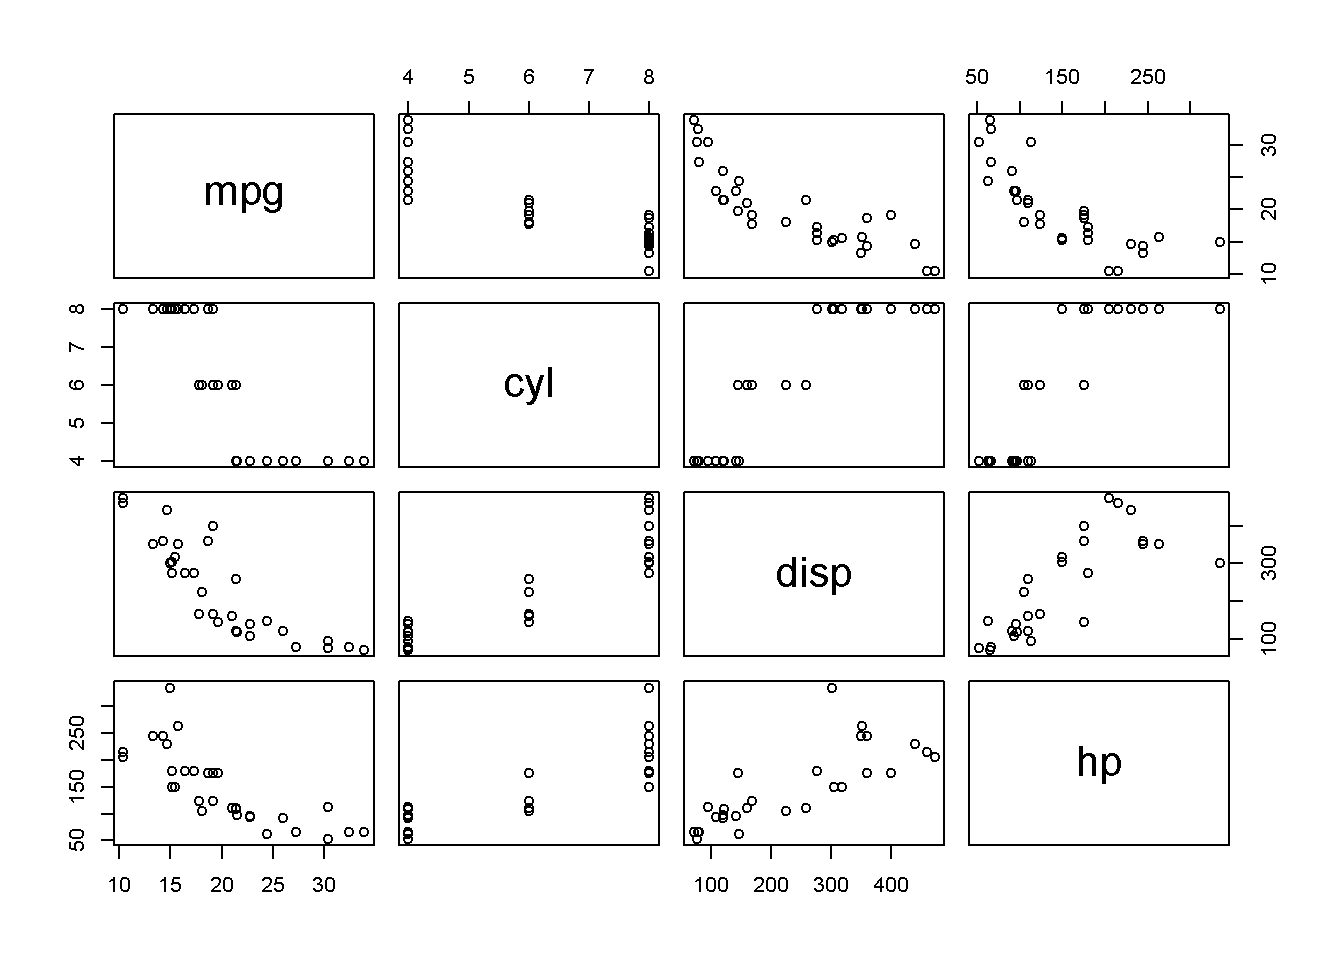
\includegraphics[keepaspectratio]{week3_files/figure-pdf/unnamed-chunk-2-1.pdf}}

Correlation Matrix

\begin{Shaded}
\begin{Highlighting}[]
\FunctionTok{cor}\NormalTok{(mtcars)}
\end{Highlighting}
\end{Shaded}

\begin{verbatim}
            mpg        cyl       disp         hp        drat         wt
mpg   1.0000000 -0.8521620 -0.8475514 -0.7761684  0.68117191 -0.8676594
cyl  -0.8521620  1.0000000  0.9020329  0.8324475 -0.69993811  0.7824958
disp -0.8475514  0.9020329  1.0000000  0.7909486 -0.71021393  0.8879799
hp   -0.7761684  0.8324475  0.7909486  1.0000000 -0.44875912  0.6587479
drat  0.6811719 -0.6999381 -0.7102139 -0.4487591  1.00000000 -0.7124406
wt   -0.8676594  0.7824958  0.8879799  0.6587479 -0.71244065  1.0000000
qsec  0.4186840 -0.5912421 -0.4336979 -0.7082234  0.09120476 -0.1747159
vs    0.6640389 -0.8108118 -0.7104159 -0.7230967  0.44027846 -0.5549157
am    0.5998324 -0.5226070 -0.5912270 -0.2432043  0.71271113 -0.6924953
gear  0.4802848 -0.4926866 -0.5555692 -0.1257043  0.69961013 -0.5832870
carb -0.5509251  0.5269883  0.3949769  0.7498125 -0.09078980  0.4276059
            qsec         vs          am       gear        carb
mpg   0.41868403  0.6640389  0.59983243  0.4802848 -0.55092507
cyl  -0.59124207 -0.8108118 -0.52260705 -0.4926866  0.52698829
disp -0.43369788 -0.7104159 -0.59122704 -0.5555692  0.39497686
hp   -0.70822339 -0.7230967 -0.24320426 -0.1257043  0.74981247
drat  0.09120476  0.4402785  0.71271113  0.6996101 -0.09078980
wt   -0.17471588 -0.5549157 -0.69249526 -0.5832870  0.42760594
qsec  1.00000000  0.7445354 -0.22986086 -0.2126822 -0.65624923
vs    0.74453544  1.0000000  0.16834512  0.2060233 -0.56960714
am   -0.22986086  0.1683451  1.00000000  0.7940588  0.05753435
gear -0.21268223  0.2060233  0.79405876  1.0000000  0.27407284
carb -0.65624923 -0.5696071  0.05753435  0.2740728  1.00000000
\end{verbatim}

Heatmap

\begin{Shaded}
\begin{Highlighting}[]
\FunctionTok{heatmap}\NormalTok{(}\FunctionTok{cor}\NormalTok{(mtcars), }\AttributeTok{main=}\StringTok{"Correlation Heatmap"}\NormalTok{)}
\end{Highlighting}
\end{Shaded}

\pandocbounded{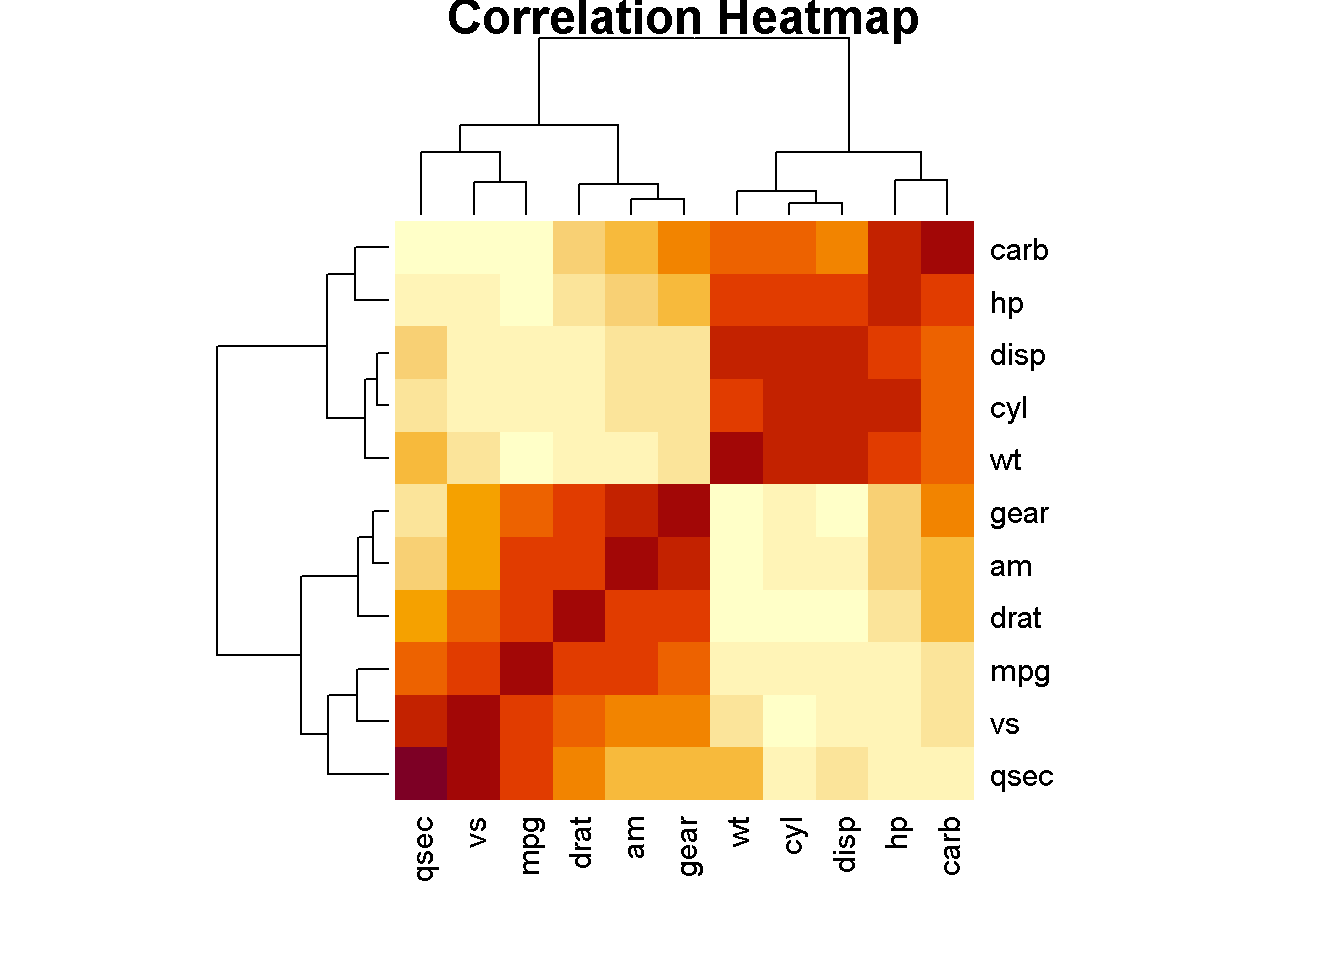
\includegraphics[keepaspectratio]{week3_files/figure-pdf/unnamed-chunk-4-1.pdf}}

\subsection{Common R Packages for
Statistics}\label{common-r-packages-for-statistics}

Package \textbar Purpose ggplot2 \textbar Data visualization dplyr
\textbar Data manipulation tidyr \textbar Data tidying Hmisc
\textbar Misc stats functions car \textbar Regression diagnostics e1071
\textbar Skewness/kurtosis, ML tools psych \textbar Psychological
statistics shiny \textbar Interactive apps caret \textbar Classification
and regression

\subsection{Introduction to Command
Line}\label{introduction-to-command-line}

\section{Windows Terminal}\label{windows-terminal}

\[
cd ..
mkdir my_project
dir
\] \#\#\# Linux Terminal \[
cd ~
mkdir stats_project
ls -l
\]

\subsection{Git + R Project Example}\label{git-r-project-example}

\[
git init
git clone https://github.com/username/project.git
\]

\subsection{Fallacies and Bias: Real-World
Cautions}\label{fallacies-and-bias-real-world-cautions}

Examples of Statistical Abuse

Cherry-picking data Data dredging (p-hacking) Using relative risk
without absolute context Non-random sampling Ethics in Data Analysis

Be transparent Document sources Disclose methodology Avoid overstating
conclusions

\subsection{Future Applications of
Statistics}\label{future-applications-of-statistics}

Real-World Domains

Healthcare: Drug effectiveness, diagnostics Economics: Forecasting,
policy evaluation Sociology: Survey analysis Sports: Performance
analytics AI/ML: Predictive modeling, optimization Next Steps

Learn tidyverse ecosystem Explore machine learning in R Build Shiny
dashboards Get familiar with reproducible research using Quarto

\subsection{Practice Challenges}\label{practice-challenges}

\begin{enumerate}
\def\labelenumi{\arabic{enumi}.}
\tightlist
\item
  Load and summarize data
\end{enumerate}

Load mtcars or your own dataset Use summary(), mean(), sd() 2. Create 3
different plots

Histogram Boxplot by group Scatter plot with trend line 3. Build a
regression model

Identify predictor and outcome Use lm() and summary() 4. Explore a GUI
like RKWard or Rcmdr

\subsection{Key Takeaways}\label{key-takeaways}

Statistics supports informed decision-making. R and its GUI frontends
offer flexibility + power. Understand theory → then automate with code.
Avoid fallacies by following robust methods. Visuals are crucial: plot
early, plot often.

\bookmarksetup{startatroot}

\chapter{Week 4}\label{week-4}

\section{Introduction}\label{introduction-3}

This eBook is a comprehensive companion to the course \emph{Basic
Statistics using GUI-R (RKWard)}. It includes foundational theory,
practical examples, and step-by-step explanations, with integrated GUI-R
usage.

\section{Course Overview}\label{course-overview}

\subsection{Course Name}\label{course-name}

\textbf{Basic Statistics using GUI-R (RKWard)}

\subsection{Instructor Profile}\label{instructor-profile}

Dr.~Harsh Pradhan is Assistant Professor at the Institute of Management
Studies, Banaras Hindu University.\\
📎 \href{https://bhu.ac.in/Site/FacultyProfile/1_5?FA000562}{Faculty
Profile}

\subsection{Learning Objectives}\label{learning-objectives}

\begin{itemize}
\tightlist
\item
  Understand core concepts in statistics
\item
  Apply t-tests and ANOVA using real data
\item
  Compute confidence intervals and test statistics
\item
  Use GUI-R (RKWard) for statistical analysis
\end{itemize}

\section{Chapter 1: Fundamental
Concepts}\label{chapter-1-fundamental-concepts}

\subsection{Descriptive Statistics}\label{descriptive-statistics-2}

\subsubsection{Central Tendency}\label{central-tendency}

\begin{itemize}
\tightlist
\item
  \textbf{Mean}\\
\item
  \textbf{Median}\\
\item
  \textbf{Mode}
\end{itemize}

\subsubsection{Dispersion}\label{dispersion}

\begin{itemize}
\tightlist
\item
  \textbf{Range}\\
\item
  \textbf{Variance}\\
\item
  \textbf{Standard Deviation}
\end{itemize}

\subsubsection{Example:}\label{example-9}

\begin{Shaded}
\begin{Highlighting}[]
\NormalTok{data }\OtherTok{\textless{}{-}} \FunctionTok{c}\NormalTok{(}\DecValTok{4}\NormalTok{, }\DecValTok{8}\NormalTok{, }\DecValTok{6}\NormalTok{, }\DecValTok{5}\NormalTok{, }\DecValTok{3}\NormalTok{)}
\FunctionTok{mean}\NormalTok{(data)}
\end{Highlighting}
\end{Shaded}

\begin{verbatim}
[1] 5.2
\end{verbatim}

\begin{Shaded}
\begin{Highlighting}[]
\FunctionTok{median}\NormalTok{(data)}
\end{Highlighting}
\end{Shaded}

\begin{verbatim}
[1] 5
\end{verbatim}

\begin{Shaded}
\begin{Highlighting}[]
\FunctionTok{sd}\NormalTok{(data)}
\end{Highlighting}
\end{Shaded}

\begin{verbatim}
[1] 1.923538
\end{verbatim}

\subsection{Standard Error}\label{standard-error}

\[
SE = \frac{s}{\sqrt{n}}
\]

Small SE = sample mean is a good estimate of the population mean.

\subsection{Central Limit Theorem}\label{central-limit-theorem}

For \(n > 30\), sampling distribution of the mean approximates normal:

\[
\bar{X} \sim \mathcal{N}(\mu, \frac{\sigma}{\sqrt{n}})
\]

\subsection{Confidence Intervals}\label{confidence-intervals}

\[
CI = \bar{x} \pm Z \cdot \frac{s}{\sqrt{n}}
\]

Interpret 95\% CI as: 95 of 100 such intervals would contain the true
mean.

\section{Chapter 2: Estimation}\label{chapter-2-estimation}

\subsection{Types of Estimates}\label{types-of-estimates}

\begin{longtable}[]{@{}lll@{}}
\toprule\noalign{}
Type & Description & Example \\
\midrule\noalign{}
\endhead
\bottomrule\noalign{}
\endlastfoot
Point Estimate & Single value & Sample mean \\
Interval Estimate & Range + confidence & Confidence Int \\
\end{longtable}

\subsection{Parameter vs Statistic}\label{parameter-vs-statistic}

\begin{longtable}[]{@{}ll@{}}
\toprule\noalign{}
Term & Description \\
\midrule\noalign{}
\endhead
\bottomrule\noalign{}
\endlastfoot
Parameter & Value from population (e.g., \(\mu\)) \\
Statistic & Value from sample (e.g., \(\bar{x}\)) \\
\end{longtable}

\section{Chapter 3: Hypothesis
Testing}\label{chapter-3-hypothesis-testing}

\begin{itemize}
\tightlist
\item
  \textbf{Null Hypothesis (\(H_0\))}: No effect\\
\item
  \textbf{Alternative Hypothesis (\(H_1\))}: Some effect\\
\item
  \textbf{Type I Error}: Reject \(H_0\) when true\\
\item
  \textbf{Type II Error}: Fail to reject \(H_0\) when false
\end{itemize}

\section{Chapter 4: Student's T-Test}\label{chapter-4-students-t-test}

\subsection{Types}\label{types}

\begin{longtable}[]{@{}ll@{}}
\toprule\noalign{}
Test Type & Description \\
\midrule\noalign{}
\endhead
\bottomrule\noalign{}
\endlastfoot
One-Sample & Compare sample to fixed value \\
Independent & Compare two unrelated groups \\
Paired & Compare two related groups \\
\end{longtable}

\subsection{One-Sample T-Test Example}\label{one-sample-t-test-example}

\begin{Shaded}
\begin{Highlighting}[]
\NormalTok{data }\OtherTok{\textless{}{-}} \FunctionTok{c}\NormalTok{(}\DecValTok{22}\NormalTok{, }\DecValTok{24}\NormalTok{, }\DecValTok{27}\NormalTok{, }\DecValTok{26}\NormalTok{, }\DecValTok{28}\NormalTok{, }\DecValTok{23}\NormalTok{, }\DecValTok{25}\NormalTok{, }\DecValTok{29}\NormalTok{, }\DecValTok{21}\NormalTok{, }\DecValTok{26}\NormalTok{, }\DecValTok{24}\NormalTok{, }\DecValTok{27}\NormalTok{)}
\FunctionTok{t.test}\NormalTok{(data, }\AttributeTok{mu =} \DecValTok{25}\NormalTok{)}
\end{Highlighting}
\end{Shaded}

\begin{verbatim}

    One Sample t-test

data:  data
t = 0.2363, df = 11, p-value = 0.8175
alternative hypothesis: true mean is not equal to 25
95 percent confidence interval:
 23.61427 26.71906
sample estimates:
mean of x 
 25.16667 
\end{verbatim}

\subsection{Test Statistic}\label{test-statistic}

\[
t = \frac{\bar{x} - \mu}{SE}
\]

\subsection{Degrees of Freedom}\label{degrees-of-freedom}

\[
df = n - 1
\]

\subsection{Decision Rule}\label{decision-rule}

Compare calculated \(t\) to table value. If \(|t| > t_{critical}\),
reject \(H_0\).

\subsection{T-Test in GUI-R}\label{t-test-in-gui-r}

\begin{enumerate}
\def\labelenumi{\arabic{enumi}.}
\tightlist
\item
  Import data\\
\item
  Choose T-Test\\
\item
  Define groups\\
\item
  Run \& interpret output
\end{enumerate}

\section{Chapter 5: ANOVA}\label{chapter-5-anova}

\subsection{Purpose}\label{purpose-1}

Used when comparing means across 3+ groups.

\subsubsection{One-Way ANOVA Formula}\label{one-way-anova-formula}

\[
F = \frac{MS_{between}}{MS_{within}}
\]

Where:

\begin{itemize}
\tightlist
\item
  \(MS_{between} = \frac{SS_{between}}{df_{between}}\)\\
\item
  \(MS_{within} = \frac{SS_{within}}{df_{within}}\)
\end{itemize}

\subsubsection{Assumptions}\label{assumptions}

\begin{itemize}
\tightlist
\item
  Normality\\
\item
  Homogeneity of variance\\
\item
  Independence
\end{itemize}

\subsubsection{Example Table}\label{example-table}

\begin{longtable}[]{@{}llll@{}}
\toprule\noalign{}
Group & Mean & Var & n \\
\midrule\noalign{}
\endhead
\bottomrule\noalign{}
\endlastfoot
A & 5.5 & 1.5 & 30 \\
B & 7.1 & 2.0 & 30 \\
C & 6.8 & 1.8 & 30 \\
\end{longtable}

\subsection{Post-Hoc Tests}\label{post-hoc-tests}

Run if ANOVA is significant to locate pairwise differences.

\subsection{ANOVA in GUI-R}\label{anova-in-gui-r}

\begin{enumerate}
\def\labelenumi{\arabic{enumi}.}
\tightlist
\item
  Load data\\
\item
  Choose ``One-Way ANOVA''\\
\item
  Define groups\\
\item
  Interpret output
\end{enumerate}

\section{Chapter 6: GUI-R Workflow}\label{chapter-6-gui-r-workflow}

\begin{enumerate}
\def\labelenumi{\arabic{enumi}.}
\tightlist
\item
  \textbf{Import Data} (CSV, Excel)\\
\item
  \textbf{Choose Test} (T-Test, ANOVA, etc.)\\
\item
  \textbf{Run} the analysis\\
\item
  \textbf{Interpret} the output\\
\item
  \textbf{Export} the results or visualizations
\end{enumerate}

\section{Chapter 7: Advanced
Concepts}\label{chapter-7-advanced-concepts}

\subsection{Variance Partitioning}\label{variance-partitioning}

\[
\text{Total Variance} = \text{Explained Variance} + \text{Unexplained Variance}
\]

\begin{longtable}[]{@{}ll@{}}
\toprule\noalign{}
Explained Terms & Unexplained Terms \\
\midrule\noalign{}
\endhead
\bottomrule\noalign{}
\endlastfoot
Systematic & Random \\
Predictive & Error \\
Deterministic & Noise \\
\end{longtable}

\subsection{Degrees of Freedom}\label{degrees-of-freedom-1}

For equation \(x + y + z = 3\), if 2 values are known, third is fixed.\\
Hence, \(df = n - k\) where \(n\) = total variables, \(k\) =
constraints.

\subsection{Chi-Square and F
Distribution}\label{chi-square-and-f-distribution}

\begin{itemize}
\tightlist
\item
  \textbf{Chi-Square}: Categorical variable comparison\\
\item
  \textbf{F-Distribution}: Used in ANOVA, variance testing
\end{itemize}

\subsection{Univariate, Bivariate,
Multivariate}\label{univariate-bivariate-multivariate}

\begin{longtable}[]{@{}lll@{}}
\toprule\noalign{}
Type & Variables & Example \\
\midrule\noalign{}
\endhead
\bottomrule\noalign{}
\endlastfoot
Univariate & 1 & Height \\
Bivariate & 2 & Height vs Weight \\
Multivariate & \textgreater2 & Study w/ Age, Gender, Income \\
\end{longtable}

\subsection{Parametric Test
Assumptions}\label{parametric-test-assumptions}

\begin{itemize}
\tightlist
\item
  Interval/Ratio DV\\
\item
  Random Sampling\\
\item
  Normality\\
\item
  Equal Variances
\end{itemize}

If assumptions violated → use non-parametric test.

\subsection{Effect Size}\label{effect-size}

\[
\text{Effect Size} = \frac{|\mu_1 - \mu_2|}{\sigma}
\]

Used for comparison across studies.

\subsection{Power of a Test}\label{power-of-a-test}

\[
\text{Power} = 1 - \beta
\]

Higher power → lower chance of Type II error\\
Power increases with sample size, effect size

\section{Conclusion}\label{conclusion}

Statistics is the language of data. GUI-R makes statistical tools
accessible for everyone. This book empowers you to analyze data
effectively using t-tests, ANOVA, and confidence intervals in a GUI
environment.

\section{References}\label{references}

\begin{itemize}
\tightlist
\item
  Pradhan, H. (2023). \emph{Basic Statistics using GUI-R (RKWard)}\\
\item
  Field, A. (2013). \emph{Discovering Statistics Using R}.\\
\item
  \url{https://methods.sagepub.com}
\end{itemize}

\section{Chapter 8: Advanced T-Test
Applications}\label{chapter-8-advanced-t-test-applications}

\subsection{Paired Sample T-Test}\label{paired-sample-t-test}

Used when the same group is measured twice (e.g., before and after).

\subsubsection{Example:}\label{example-10}

\begin{Shaded}
\begin{Highlighting}[]
\NormalTok{before }\OtherTok{\textless{}{-}} \FunctionTok{c}\NormalTok{(}\DecValTok{80}\NormalTok{, }\DecValTok{82}\NormalTok{, }\DecValTok{79}\NormalTok{, }\DecValTok{84}\NormalTok{, }\DecValTok{88}\NormalTok{)}
\NormalTok{after }\OtherTok{\textless{}{-}} \FunctionTok{c}\NormalTok{(}\DecValTok{78}\NormalTok{, }\DecValTok{81}\NormalTok{, }\DecValTok{76}\NormalTok{, }\DecValTok{83}\NormalTok{, }\DecValTok{86}\NormalTok{)}
\FunctionTok{t.test}\NormalTok{(before, after, }\AttributeTok{paired =} \ConstantTok{TRUE}\NormalTok{)}
\end{Highlighting}
\end{Shaded}

\begin{verbatim}

    Paired t-test

data:  before and after
t = 4.8107, df = 4, p-value = 0.008581
alternative hypothesis: true mean difference is not equal to 0
95 percent confidence interval:
 0.7611494 2.8388506
sample estimates:
mean difference 
            1.8 
\end{verbatim}

\subsection{Independent Samples
T-Test}\label{independent-samples-t-test}

Compare means of two unrelated groups.

\begin{Shaded}
\begin{Highlighting}[]
\NormalTok{group1 }\OtherTok{\textless{}{-}} \FunctionTok{c}\NormalTok{(}\DecValTok{85}\NormalTok{, }\DecValTok{90}\NormalTok{, }\DecValTok{88}\NormalTok{, }\DecValTok{92}\NormalTok{, }\DecValTok{87}\NormalTok{)}
\NormalTok{group2 }\OtherTok{\textless{}{-}} \FunctionTok{c}\NormalTok{(}\DecValTok{80}\NormalTok{, }\DecValTok{83}\NormalTok{, }\DecValTok{85}\NormalTok{, }\DecValTok{84}\NormalTok{, }\DecValTok{82}\NormalTok{)}
\FunctionTok{t.test}\NormalTok{(group1, group2)}
\end{Highlighting}
\end{Shaded}

\begin{verbatim}

    Welch Two Sample t-test

data:  group1 and group2
t = 3.7755, df = 7.226, p-value = 0.006537
alternative hypothesis: true difference in means is not equal to 0
95 percent confidence interval:
 2.114814 9.085186
sample estimates:
mean of x mean of y 
     88.4      82.8 
\end{verbatim}

\subsection{One-Sample T-Test with
GUI-R}\label{one-sample-t-test-with-gui-r}

\begin{itemize}
\tightlist
\item
  Import dataset
\item
  Use `Descriptive Statistics' to check mean
\item
  Navigate to `T-Test' → `One Sample'
\item
  Input hypothesized mean and run
\end{itemize}

\section{Chapter 9: More on Confidence
Intervals}\label{chapter-9-more-on-confidence-intervals}

\subsection{Visualizing Confidence Intervals in
R}\label{visualizing-confidence-intervals-in-r}

\begin{Shaded}
\begin{Highlighting}[]
\NormalTok{x }\OtherTok{\textless{}{-}} \FunctionTok{c}\NormalTok{(}\DecValTok{88}\NormalTok{, }\DecValTok{90}\NormalTok{, }\DecValTok{85}\NormalTok{, }\DecValTok{87}\NormalTok{, }\DecValTok{89}\NormalTok{)}
\NormalTok{mean\_x }\OtherTok{\textless{}{-}} \FunctionTok{mean}\NormalTok{(x)}
\NormalTok{se }\OtherTok{\textless{}{-}} \FunctionTok{sd}\NormalTok{(x) }\SpecialCharTok{/} \FunctionTok{sqrt}\NormalTok{(}\FunctionTok{length}\NormalTok{(x))}
\NormalTok{ci\_lower }\OtherTok{\textless{}{-}}\NormalTok{ mean\_x }\SpecialCharTok{{-}} \FloatTok{1.96} \SpecialCharTok{*}\NormalTok{ se}
\NormalTok{ci\_upper }\OtherTok{\textless{}{-}}\NormalTok{ mean\_x }\SpecialCharTok{+} \FloatTok{1.96} \SpecialCharTok{*}\NormalTok{ se}
\FunctionTok{c}\NormalTok{(ci\_lower, ci\_upper)}
\end{Highlighting}
\end{Shaded}

\begin{verbatim}
[1] 86.11394 89.48606
\end{verbatim}

Plot using \texttt{ggplot2}:

\begin{Shaded}
\begin{Highlighting}[]
\FunctionTok{library}\NormalTok{(ggplot2)}
\NormalTok{df }\OtherTok{\textless{}{-}} \FunctionTok{data.frame}\NormalTok{(}\AttributeTok{x =}\NormalTok{ x)}
\FunctionTok{ggplot}\NormalTok{(df, }\FunctionTok{aes}\NormalTok{(}\AttributeTok{y =}\NormalTok{ x, }\AttributeTok{x =} \DecValTok{1}\NormalTok{)) }\SpecialCharTok{+}
  \FunctionTok{geom\_point}\NormalTok{() }\SpecialCharTok{+}
  \FunctionTok{geom\_errorbar}\NormalTok{(}\FunctionTok{aes}\NormalTok{(}\AttributeTok{ymin =}\NormalTok{ ci\_lower, }\AttributeTok{ymax =}\NormalTok{ ci\_upper), }\AttributeTok{width =} \FloatTok{0.1}\NormalTok{)}
\end{Highlighting}
\end{Shaded}

\pandocbounded{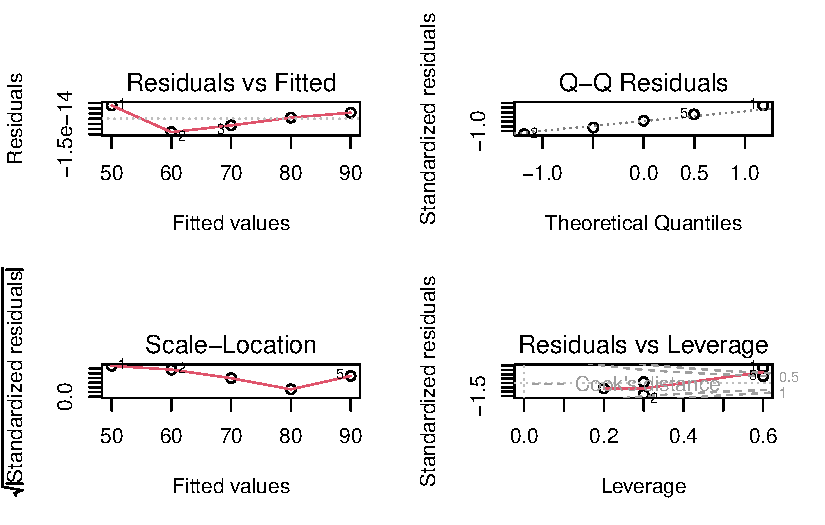
\includegraphics[keepaspectratio]{week4_files/figure-pdf/unnamed-chunk-6-1.pdf}}

\section{Chapter 10: Robust ANOVA
Models}\label{chapter-10-robust-anova-models}

\subsection{Two-Way ANOVA}\label{two-way-anova}

Examines the effect of two categorical independent variables on a
continuous dependent variable.

\begin{Shaded}
\begin{Highlighting}[]
\CommentTok{\# Sample dataset for demonstration}
\NormalTok{dataset }\OtherTok{\textless{}{-}} \FunctionTok{data.frame}\NormalTok{(}
  \AttributeTok{score =} \FunctionTok{c}\NormalTok{(}\DecValTok{85}\NormalTok{, }\DecValTok{90}\NormalTok{, }\DecValTok{88}\NormalTok{, }\DecValTok{92}\NormalTok{, }\DecValTok{87}\NormalTok{, }\DecValTok{80}\NormalTok{, }\DecValTok{83}\NormalTok{, }\DecValTok{85}\NormalTok{, }\DecValTok{84}\NormalTok{, }\DecValTok{82}\NormalTok{),}
  \AttributeTok{gender =} \FunctionTok{rep}\NormalTok{(}\FunctionTok{c}\NormalTok{(}\StringTok{"Male"}\NormalTok{, }\StringTok{"Female"}\NormalTok{), }\AttributeTok{each =} \DecValTok{5}\NormalTok{),}
  \AttributeTok{teaching\_method =} \FunctionTok{rep}\NormalTok{(}\FunctionTok{c}\NormalTok{(}\StringTok{"A"}\NormalTok{, }\StringTok{"B"}\NormalTok{), }\AttributeTok{times =} \DecValTok{5}\NormalTok{)}
\NormalTok{)}
\NormalTok{aov\_result }\OtherTok{\textless{}{-}} \FunctionTok{aov}\NormalTok{(score }\SpecialCharTok{\textasciitilde{}}\NormalTok{ gender }\SpecialCharTok{*}\NormalTok{ teaching\_method, }\AttributeTok{data =}\NormalTok{ dataset)}
\FunctionTok{summary}\NormalTok{(aov\_result)}
\end{Highlighting}
\end{Shaded}

\begin{verbatim}
                       Df Sum Sq Mean Sq F value  Pr(>F)   
gender                  1  78.40   78.40  23.718 0.00279 **
teaching_method         1   6.02    6.02   1.820 0.22598   
gender:teaching_method  1  18.15   18.15   5.491 0.05759 . 
Residuals               6  19.83    3.31                   
---
Signif. codes:  0 '***' 0.001 '**' 0.01 '*' 0.05 '.' 0.1 ' ' 1
\end{verbatim}

\subsection{Repeated Measures ANOVA}\label{repeated-measures-anova}

Use when the same subjects are used for each treatment.

\begin{Shaded}
\begin{Highlighting}[]
\CommentTok{\# Sample repeated measures data in long format}
\NormalTok{data\_long }\OtherTok{\textless{}{-}} \FunctionTok{data.frame}\NormalTok{(}
  \AttributeTok{id =} \FunctionTok{rep}\NormalTok{(}\DecValTok{1}\SpecialCharTok{:}\DecValTok{5}\NormalTok{, }\AttributeTok{each =} \DecValTok{3}\NormalTok{),}
  \AttributeTok{condition =} \FunctionTok{rep}\NormalTok{(}\FunctionTok{c}\NormalTok{(}\StringTok{"A"}\NormalTok{, }\StringTok{"B"}\NormalTok{, }\StringTok{"C"}\NormalTok{), }\AttributeTok{times =} \DecValTok{5}\NormalTok{),}
  \AttributeTok{score =} \FunctionTok{c}\NormalTok{(}\DecValTok{85}\NormalTok{, }\DecValTok{88}\NormalTok{, }\DecValTok{90}\NormalTok{, }\DecValTok{80}\NormalTok{, }\DecValTok{82}\NormalTok{, }\DecValTok{85}\NormalTok{, }\DecValTok{78}\NormalTok{, }\DecValTok{80}\NormalTok{, }\DecValTok{83}\NormalTok{, }\DecValTok{90}\NormalTok{, }\DecValTok{92}\NormalTok{, }\DecValTok{95}\NormalTok{, }\DecValTok{88}\NormalTok{, }\DecValTok{90}\NormalTok{, }\DecValTok{91}\NormalTok{)}
\NormalTok{)}
\FunctionTok{library}\NormalTok{(ez)}
\FunctionTok{ezANOVA}\NormalTok{(}\AttributeTok{data =}\NormalTok{ data\_long, }\AttributeTok{dv =}\NormalTok{ .(score), }\AttributeTok{wid =}\NormalTok{ .(id), }\AttributeTok{within =}\NormalTok{ .(condition))}
\end{Highlighting}
\end{Shaded}

\begin{verbatim}
Warning: Converting "id" to factor for ANOVA.
\end{verbatim}

\begin{verbatim}
Warning: Converting "condition" to factor for ANOVA.
\end{verbatim}

\begin{verbatim}
$ANOVA
     Effect DFn DFd        F            p p<.05       ges
2 condition   2   8 88.22222 3.539139e-06     * 0.1479687

$`Mauchly's Test for Sphericity`
     Effect         W         p p<.05
2 condition 0.5555556 0.4140867      

$`Sphericity Corrections`
     Effect       GGe        p[GG] p[GG]<.05       HFe        p[HF] p[HF]<.05
2 condition 0.6923077 9.135419e-05         * 0.9411765 6.568851e-06         *
\end{verbatim}

\section{Chapter 11: Effect Size
Measures}\label{chapter-11-effect-size-measures}

\subsection{Cohen's d}\label{cohens-d}

\[
d = \frac{\bar{x}_1 - \bar{x}_2}{s_p}
\]

Where \(s_p\) is the pooled standard deviation.

\subsubsection{R Example}\label{r-example}

\begin{Shaded}
\begin{Highlighting}[]
\FunctionTok{library}\NormalTok{(effsize)}
\FunctionTok{cohen.d}\NormalTok{(group1, group2)}
\end{Highlighting}
\end{Shaded}

\begin{verbatim}

Cohen's d

d estimate: 2.387848 (large)
95 percent confidence interval:
    lower     upper 
0.4791634 4.2965327 
\end{verbatim}

\subsection{\texorpdfstring{Eta-Squared
(\(\eta^2\))}{Eta-Squared (\textbackslash eta\^{}2)}}\label{eta-squared-eta2}

Used for ANOVA:

\[
\eta^2 = \frac{SS_{between}}{SS_{total}}
\]

\section{Chapter 12: Statistical Assumptions
Checking}\label{chapter-12-statistical-assumptions-checking}

\subsection{Normality}\label{normality}

Use Shapiro-Wilk test:

\begin{Shaded}
\begin{Highlighting}[]
\CommentTok{\# Sample data frame for normality test}
\NormalTok{data }\OtherTok{\textless{}{-}} \FunctionTok{data.frame}\NormalTok{(}\AttributeTok{variable =} \FunctionTok{c}\NormalTok{(}\DecValTok{88}\NormalTok{, }\DecValTok{90}\NormalTok{, }\DecValTok{85}\NormalTok{, }\DecValTok{87}\NormalTok{, }\DecValTok{89}\NormalTok{, }\DecValTok{91}\NormalTok{, }\DecValTok{92}\NormalTok{, }\DecValTok{88}\NormalTok{, }\DecValTok{90}\NormalTok{, }\DecValTok{87}\NormalTok{))}
\FunctionTok{shapiro.test}\NormalTok{(data}\SpecialCharTok{$}\NormalTok{variable)}
\end{Highlighting}
\end{Shaded}

\begin{verbatim}

    Shapiro-Wilk normality test

data:  data$variable
W = 0.97743, p-value = 0.95
\end{verbatim}

Visualize:

\begin{Shaded}
\begin{Highlighting}[]
\FunctionTok{qqnorm}\NormalTok{(data}\SpecialCharTok{$}\NormalTok{variable)}
\FunctionTok{qqline}\NormalTok{(data}\SpecialCharTok{$}\NormalTok{variable)}
\end{Highlighting}
\end{Shaded}

\pandocbounded{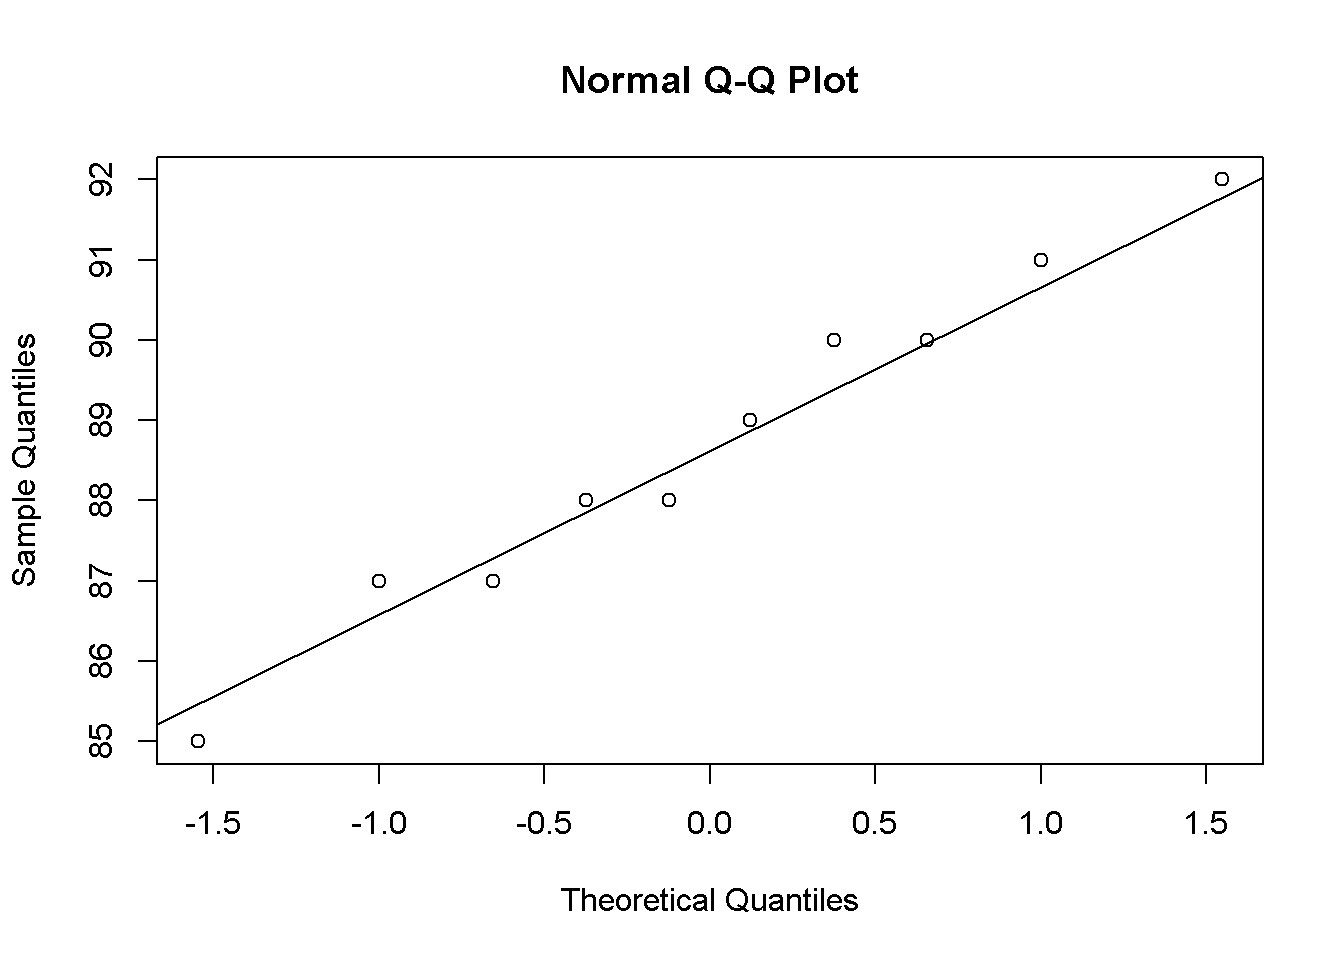
\includegraphics[keepaspectratio]{week4_files/figure-pdf/unnamed-chunk-11-1.pdf}}

\subsection{Homogeneity of Variance}\label{homogeneity-of-variance}

Use Levene's Test:

\begin{Shaded}
\begin{Highlighting}[]
\CommentTok{\# Sample data frame for Levene\textquotesingle{}s Test}
\NormalTok{data }\OtherTok{\textless{}{-}} \FunctionTok{data.frame}\NormalTok{(}
  \AttributeTok{variable =} \FunctionTok{c}\NormalTok{(}\DecValTok{88}\NormalTok{, }\DecValTok{90}\NormalTok{, }\DecValTok{85}\NormalTok{, }\DecValTok{87}\NormalTok{, }\DecValTok{89}\NormalTok{, }\DecValTok{91}\NormalTok{, }\DecValTok{92}\NormalTok{, }\DecValTok{88}\NormalTok{, }\DecValTok{90}\NormalTok{, }\DecValTok{87}\NormalTok{),}
  \AttributeTok{group =} \FunctionTok{rep}\NormalTok{(}\FunctionTok{c}\NormalTok{(}\StringTok{"A"}\NormalTok{, }\StringTok{"B"}\NormalTok{), }\AttributeTok{each =} \DecValTok{5}\NormalTok{)}
\NormalTok{)}
\FunctionTok{library}\NormalTok{(car)}
\end{Highlighting}
\end{Shaded}

\begin{verbatim}
Loading required package: carData
\end{verbatim}

\begin{Shaded}
\begin{Highlighting}[]
\FunctionTok{leveneTest}\NormalTok{(variable }\SpecialCharTok{\textasciitilde{}}\NormalTok{ group, }\AttributeTok{data =}\NormalTok{ data)}
\end{Highlighting}
\end{Shaded}

\begin{verbatim}
Warning in leveneTest.default(y = y, group = group, ...): group coerced to
factor.
\end{verbatim}

\begin{verbatim}
Levene's Test for Homogeneity of Variance (center = median)
      Df F value Pr(>F)
group  1  0.0769 0.7885
       8               
\end{verbatim}

\section{Chapter 13: Non-Parametric
Alternatives}\label{chapter-13-non-parametric-alternatives}

\subsection{Wilcoxon Signed Rank Test}\label{wilcoxon-signed-rank-test}

\begin{Shaded}
\begin{Highlighting}[]
\FunctionTok{wilcox.test}\NormalTok{(before, after, }\AttributeTok{paired =} \ConstantTok{TRUE}\NormalTok{)}
\end{Highlighting}
\end{Shaded}

\begin{verbatim}
Warning in wilcox.test.default(before, after, paired = TRUE): cannot compute
exact p-value with ties
\end{verbatim}

\begin{verbatim}

    Wilcoxon signed rank test with continuity correction

data:  before and after
V = 15, p-value = 0.05676
alternative hypothesis: true location shift is not equal to 0
\end{verbatim}

\subsection{Mann-Whitney U Test}\label{mann-whitney-u-test}

\begin{Shaded}
\begin{Highlighting}[]
\FunctionTok{wilcox.test}\NormalTok{(group1, group2)}
\end{Highlighting}
\end{Shaded}

\begin{verbatim}
Warning in wilcox.test.default(group1, group2): cannot compute exact p-value
with ties
\end{verbatim}

\begin{verbatim}

    Wilcoxon rank sum test with continuity correction

data:  group1 and group2
W = 24.5, p-value = 0.01597
alternative hypothesis: true location shift is not equal to 0
\end{verbatim}

\subsection{Kruskal-Wallis Test}\label{kruskal-wallis-test}

Non-parametric alternative to ANOVA.

\begin{Shaded}
\begin{Highlighting}[]
\CommentTok{\# Sample data frame for Kruskal{-}Wallis Test}
\NormalTok{data }\OtherTok{\textless{}{-}} \FunctionTok{data.frame}\NormalTok{(}
  \AttributeTok{score =} \FunctionTok{c}\NormalTok{(}\DecValTok{85}\NormalTok{, }\DecValTok{88}\NormalTok{, }\DecValTok{90}\NormalTok{, }\DecValTok{80}\NormalTok{, }\DecValTok{82}\NormalTok{, }\DecValTok{85}\NormalTok{, }\DecValTok{78}\NormalTok{, }\DecValTok{80}\NormalTok{, }\DecValTok{83}\NormalTok{, }\DecValTok{90}\NormalTok{, }\DecValTok{92}\NormalTok{, }\DecValTok{95}\NormalTok{, }\DecValTok{88}\NormalTok{, }\DecValTok{90}\NormalTok{, }\DecValTok{91}\NormalTok{),}
  \AttributeTok{group =} \FunctionTok{rep}\NormalTok{(}\FunctionTok{c}\NormalTok{(}\StringTok{"A"}\NormalTok{, }\StringTok{"B"}\NormalTok{, }\StringTok{"C"}\NormalTok{), }\AttributeTok{times =} \DecValTok{5}\NormalTok{)}
\NormalTok{)}
\FunctionTok{kruskal.test}\NormalTok{(score }\SpecialCharTok{\textasciitilde{}}\NormalTok{ group, }\AttributeTok{data =}\NormalTok{ data)}
\end{Highlighting}
\end{Shaded}

\begin{verbatim}

    Kruskal-Wallis rank sum test

data:  score by group
Kruskal-Wallis chi-squared = 2.2329, df = 2, p-value = 0.3274
\end{verbatim}

\section{Visualizing Statistical
Results}\label{visualizing-statistical-results}

\section{Boxplots}\label{boxplots}

\begin{Shaded}
\begin{Highlighting}[]
\FunctionTok{ggplot}\NormalTok{(data, }\FunctionTok{aes}\NormalTok{(}\AttributeTok{x =}\NormalTok{ group, }\AttributeTok{y =}\NormalTok{ score)) }\SpecialCharTok{+}
  \FunctionTok{geom\_boxplot}\NormalTok{()}
\end{Highlighting}
\end{Shaded}

\pandocbounded{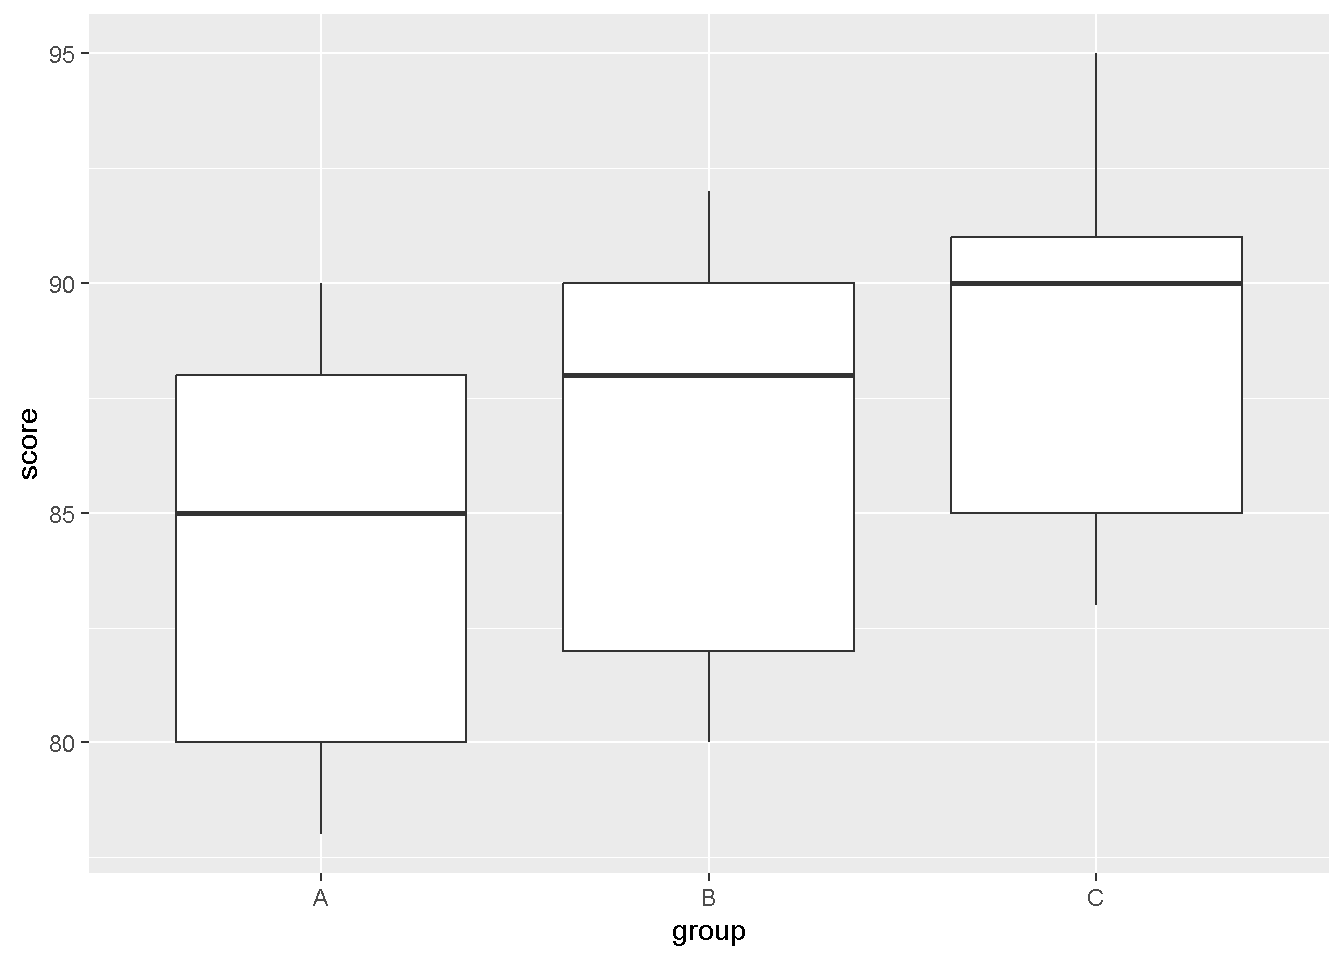
\includegraphics[keepaspectratio]{week4_files/figure-pdf/unnamed-chunk-16-1.pdf}}

\subsection{Histograms}\label{histograms}

\begin{Shaded}
\begin{Highlighting}[]
\FunctionTok{ggplot}\NormalTok{(data, }\FunctionTok{aes}\NormalTok{(}\AttributeTok{x =}\NormalTok{ score)) }\SpecialCharTok{+}
  \FunctionTok{geom\_histogram}\NormalTok{(}\AttributeTok{binwidth =} \DecValTok{2}\NormalTok{)}
\end{Highlighting}
\end{Shaded}

\pandocbounded{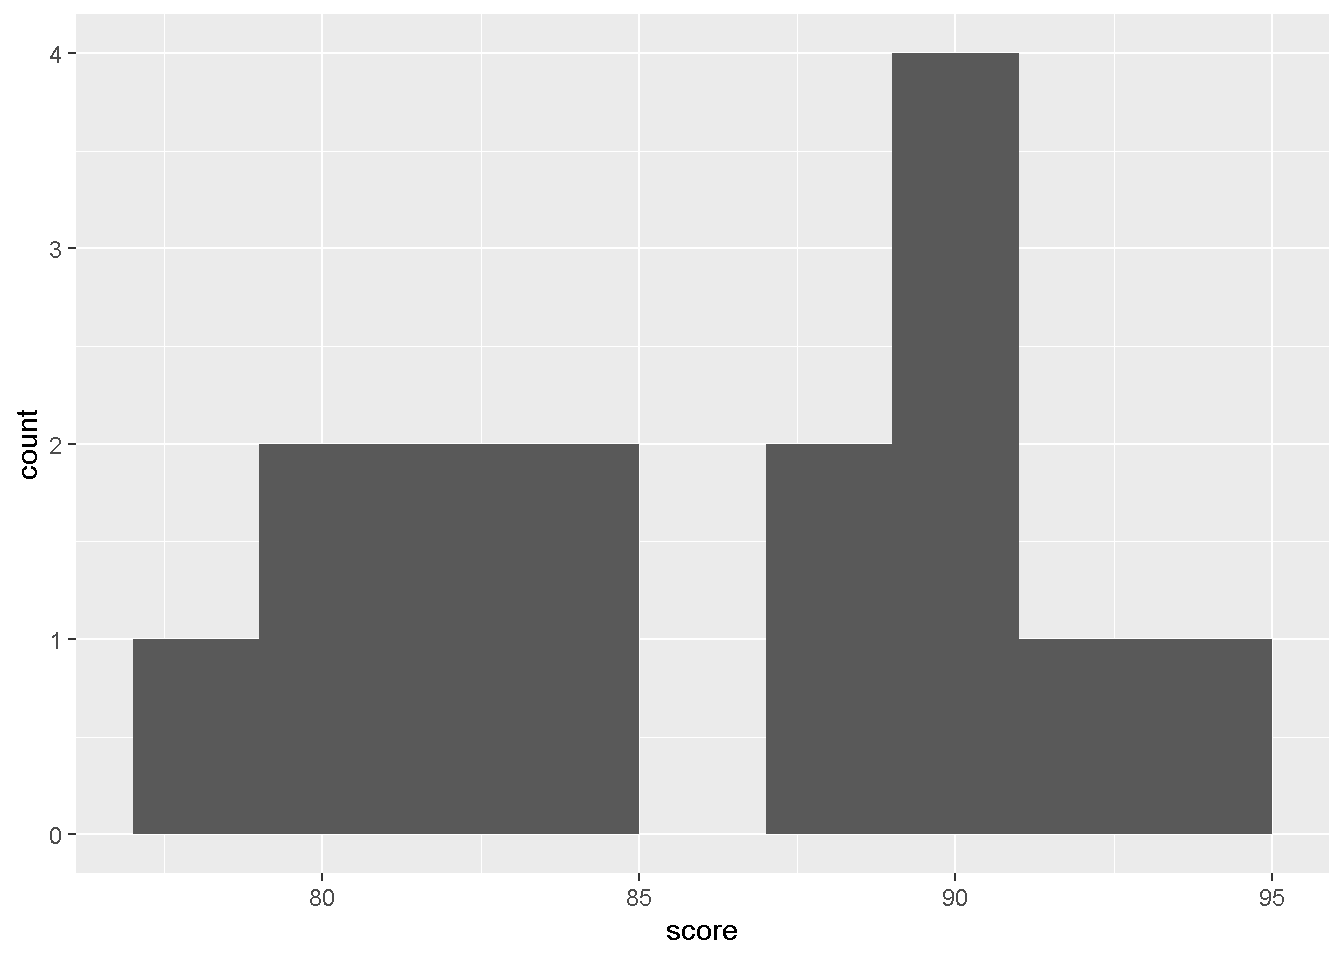
\includegraphics[keepaspectratio]{week4_files/figure-pdf/unnamed-chunk-17-1.pdf}}

\subsection{Density Plot}\label{density-plot}

\begin{Shaded}
\begin{Highlighting}[]
\FunctionTok{ggplot}\NormalTok{(data, }\FunctionTok{aes}\NormalTok{(}\AttributeTok{x =}\NormalTok{ score)) }\SpecialCharTok{+}
  \FunctionTok{geom\_density}\NormalTok{()}
\end{Highlighting}
\end{Shaded}

\pandocbounded{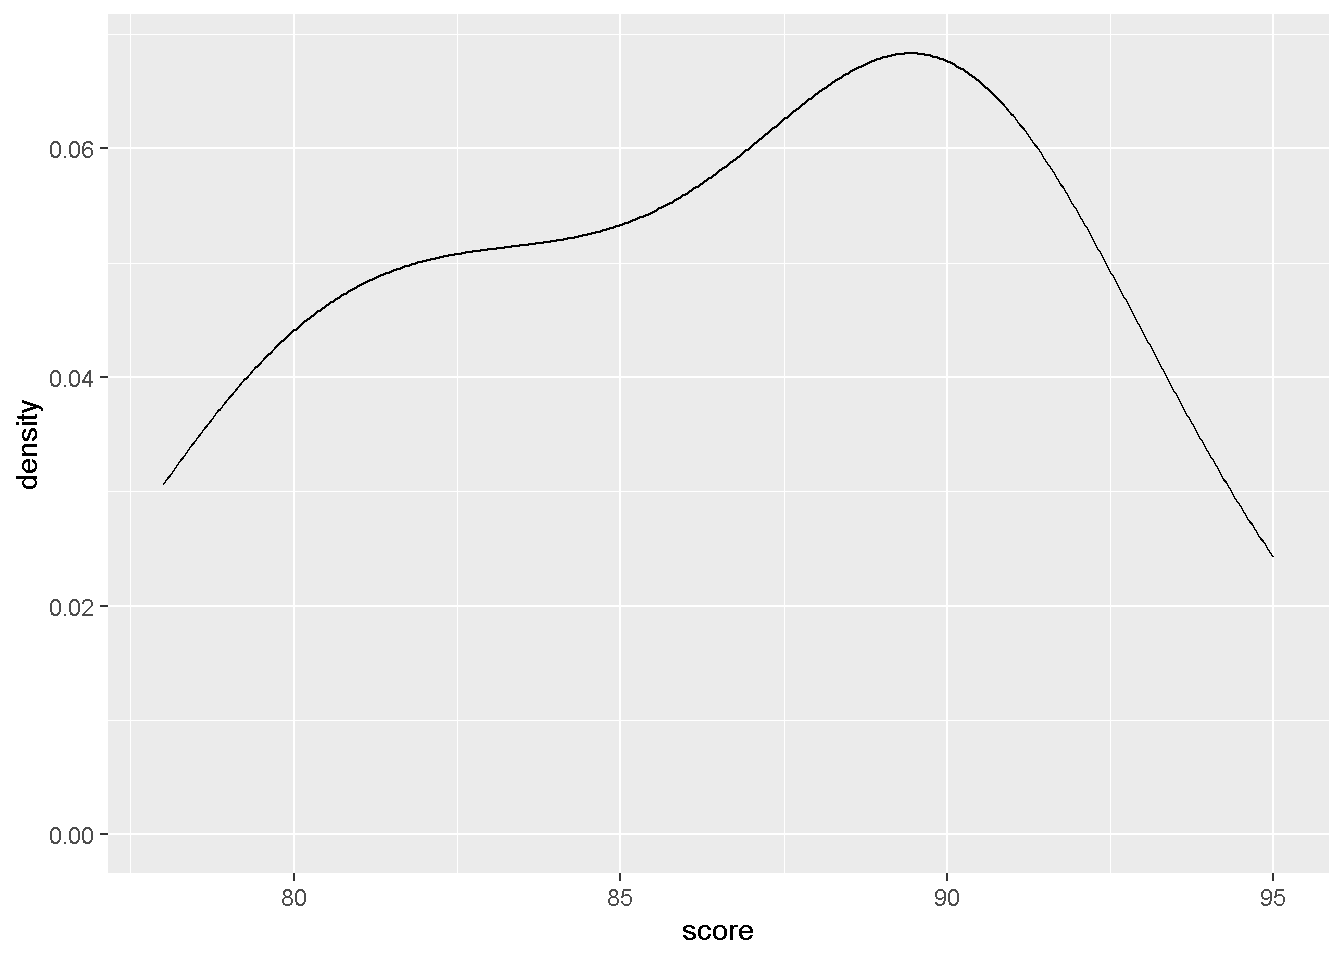
\includegraphics[keepaspectratio]{week4_files/figure-pdf/unnamed-chunk-18-1.pdf}}

\section{RKWard (GUI-R) Tips}\label{rkward-gui-r-tips}

\begin{itemize}
\tightlist
\item
  Use menu-based analysis for beginners
\item
  Save and export plots easily
\item
  Integrate with R scripts for reproducibility
\end{itemize}

\subsection{📘Summary: Basic Statistics using GUI-R
(RKWard)}\label{summary-basic-statistics-using-gui-r-rkward}

This eBook, authored by Dr.~Harsh Pradhan (Assistant Professor at the
Institute of Management Studies, Banaras Hindu University), serves as a
comprehensive guide to understanding and applying basic statistical
concepts, particularly in the GUI-based software RKWard (GUI-R).

Key Highlights: 1. Descriptive Statistics Covers measures of central
tendency (mean, median, mode) and variability (range, variance, standard
deviation). Introduces standard error and its role in estimating
population parameters. 2. Inferential Statistics Introduces the Central
Limit Theorem and how it forms the foundation for many statistical
techniques. Confidence intervals are explained both theoretically and
with practical calculations. 3. T-Tests (Student's t) Explains
one-sample, independent-sample, and paired-sample t-tests. Includes
step-by-step computation and GUI-R implementation. Includes
interpretation of p-values, degrees of freedom, and test statistics. 4.
Analysis of Variance (ANOVA) Covers one-way, two-way, and repeated
measures ANOVA. Focuses on the F-statistic, assumptions, and post-hoc
analyses. Discusses partitioning of variance into systematic and
unsystematic components. 5. Effect Size and Statistical Power Introduces
Cohen's d, eta-squared, and power analysis. Emphasizes that statistical
significance does not always imply practical importance. 6. Assumption
Testing Tests for normality (Shapiro-Wilk, QQ plot). Tests for
homogeneity of variance (Levene's test). Highlights when to use
non-parametric alternatives. 7. Non-Parametric Tests Introduces Wilcoxon
signed-rank, Mann-Whitney U, and Kruskal-Wallis tests as robust
alternatives to parametric methods. 8. Data Visualization in R
Demonstrates use of boxplots, histograms, and density plots using
ggplot2. Provides example R code for reproducibility. 9. GUI-R (RKWard)
Usage Offers practical steps for using GUI-R for all statistical
techniques covered. Designed to bridge the gap for learners unfamiliar
with command-line R.

\bookmarksetup{startatroot}

\chapter{Week 5}\label{week-5}

\section{1. Introduction}\label{introduction-4}

Welcome to \textbf{Week 5} of \emph{Basic Statistics using GUI-R
(RKWard)}, where we cover \textbf{relationship testing},
\textbf{correlation}, \textbf{regression}, \textbf{ANOVA}, and related
diagnostics in \textbf{depth}, using both theory and R-based
implementation.

This book is designed to:

\begin{itemize}
\tightlist
\item
  Clarify statistical concepts visually
\item
  Use real data simulations
\item
  Empower you with reproducible R/RKWard workflows
\item
  Prepare you to run statistical diagnostics and build interpretations
\end{itemize}

\begin{center}\rule{0.5\linewidth}{0.5pt}\end{center}

\section{2. Lecture 24 -- Deep Dive:
Correlation}\label{lecture-24-deep-dive-correlation}

\subsection{2.1 What is Correlation?}\label{what-is-correlation}

Correlation is a statistical measure that expresses the \textbf{extent
to which two variables are linearly related}.

\subsubsection{💡 Theory}\label{theory}

\begin{itemize}
\tightlist
\item
  If variable X increases as Y increases → \textbf{Positive correlation}
\item
  If variable X increases as Y decreases → \textbf{Negative correlation}
\item
  If there's no linear trend → \textbf{Zero correlation}
\end{itemize}

\begin{quote}
Pearson's r ranges from -1 to +1.
\end{quote}

\begin{center}\rule{0.5\linewidth}{0.5pt}\end{center}

\subsection{2.2 Types of Correlation and Use
Cases}\label{types-of-correlation-and-use-cases}

\begin{longtable}[]{@{}
  >{\raggedright\arraybackslash}p{(\linewidth - 4\tabcolsep) * \real{0.2564}}
  >{\raggedright\arraybackslash}p{(\linewidth - 4\tabcolsep) * \real{0.2308}}
  >{\raggedright\arraybackslash}p{(\linewidth - 4\tabcolsep) * \real{0.5128}}@{}}
\toprule\noalign{}
\begin{minipage}[b]{\linewidth}\raggedright
Data Type
\end{minipage} & \begin{minipage}[b]{\linewidth}\raggedright
Correlation Type
\end{minipage} & \begin{minipage}[b]{\linewidth}\raggedright
Use Case Example
\end{minipage} \\
\midrule\noalign{}
\endhead
\bottomrule\noalign{}
\endlastfoot
Nominal & Phi & Gender vs.~Yes/No Preferences \\
Dichotomous & Point-Biserial & Pass/Fail vs.~Exam Score \\
Ordinal/Rank & Spearman/Kendall & Rank in class vs.~Test anxiety \\
Ratio/Interval & Pearson & Height vs.~Weight \\
Multivariate & Partial Correl. & Control confounders \\
\end{longtable}

\begin{center}\rule{0.5\linewidth}{0.5pt}\end{center}

\subsection{2.3 Pearson, Spearman, Kendall
Comparison}\label{pearson-spearman-kendall-comparison}

\{r\} \#\# Simulate linear data set.seed(123) x \textless- rnorm(100) y
\textless- 2 * x + rnorm(100)

\section{Add non-linear data}\label{add-non-linear-data}

z \textless- x\^{}2 + rnorm(100)

\section{Pearson (linear)}\label{pearson-linear}

cor(x, y, method = ``pearson'')

\section{Spearman (rank, monotonic)}\label{spearman-rank-monotonic}

cor(x, z, method = ``spearman'')

\section{Kendall (ordinal)}\label{kendall-ordinal}

cor(x, z, method = ``kendall'') 2.4 Visualizing Correlations \#\#
Visualization library(ggplot2) data \textless- data.frame(x, y, z)

ggplot(data, aes(x = x, y = y)) + geom\_point() + geom\_smooth(method =
``lm'', se = FALSE, color = ``blue'') + labs(title = ``Scatter Plot with
Linear Fit'', x = ``X'', y = ``Y'')

ggplot(data, aes(x = x, y = z)) + geom\_point(color = ``darkred'') +
labs(title = ``Non-Linear Relationship'', x = ``X'', y = ``Z'') 2.5
Correlation Matrix in RKWard Steps:

Load data into RKWard.

Navigate to Statistics → Summaries → Correlation Matrix.

Choose the appropriate variables.

Choose correlation type (Pearson, Spearman).

Run and interpret the matrix output.

2.6 Partial Correlation in R When you want to compute the correlation
between two variables while controlling for a third:

\section{install.packages(``ggm'')}\label{install.packagesggm}

library(ggm) X1 \textless- rnorm(100) X2 \textless- X1 + rnorm(100, sd =
0.5) X3 \textless- rnorm(100) pcor(c(``X1'', ``X2'', ``X3''),
cov(cbind(X1, X2, X3))) Interpretation: This tells you the pure
correlation between X1 and X2, controlling for X3.

2.7 R Code to Automate All

\section{Simulate data}\label{simulate-data}

set.seed(100) data \textless- data.frame( A = rnorm(100), B =
rnorm(100), C = rnorm(100) )

\section{Generate all pairwise
correlations}\label{generate-all-pairwise-correlations}

cor(data)

\section{Visualize matrix with
corrplot}\label{visualize-matrix-with-corrplot}

library(corrplot) corrplot(cor(data), method = ``color'', tl.col =
``black'', addCoef.col = ``black'') 2.8 Spearman vs Pearson -- When to
Use? Use Pearson when data is normally distributed, continuous, and
linear.

Use Spearman when data is ordinal, ranked, or non-linear but monotonic.

Kendall's Tau is more robust for small sample sizes.

👀 \textbf{Next Up: Part 2/4} will include:

\begin{itemize}
\tightlist
\item
  One-Way ANOVA full theory + math\\
\item
  Repeated Measures ANOVA (detailed)\\
\item
  Visualization of F-distributions\\
\item
  MANOVA + N-Way examples\\
\item
  10+ R code exercises
\end{itemize}

\section{3. Lecture 25 -- One-Way ANOVA
(Detailed)}\label{lecture-25-one-way-anova-detailed}

\subsection{3.1 Concept Overview}\label{concept-overview}

\textbf{Analysis of Variance (ANOVA)} is used when comparing the
\textbf{means of three or more groups}.

\subsubsection{💡 Formula Breakdown}\label{formula-breakdown}

\begin{itemize}
\tightlist
\item
  \textbf{SSM (Sum of Squares Model)}: Variation between groups
\item
  \textbf{SSR (Sum of Squares Residual)}: Variation within groups
\item
  \textbf{SST (Total)}: Total variation
\end{itemize}

\textbf{F-Ratio}:

\[
F = \frac{MS_{between}}{MS_{within}} = \frac{SSM / df_M}{SSR / df_R}
\]

\subsection{3.2 ANOVA Table Example}\label{anova-table-example}

\begin{longtable}[]{@{}lllll@{}}
\toprule\noalign{}
Source & SS & df & MS & F \\
\midrule\noalign{}
\endhead
\bottomrule\noalign{}
\endlastfoot
Between & 461.64 & 3 & 153.88 & 8.27 \\
Within & 167.42 & 9 & 18.60 & \\
Total & 629.08 & 12 & & \\
\end{longtable}

\begin{center}\rule{0.5\linewidth}{0.5pt}\end{center}

\subsection{3.3 R Code -- One-Way ANOVA}\label{r-code-one-way-anova}

group1 \textless- c(28, 36, 38, 31) group2 \textless- c(32, 33, 40)
group3 \textless- c(47, 43, 52) group4 \textless- c(40, 47, 45)

score \textless- c(group1, group2, group3, group4) group \textless-
factor(rep(c(``Hunter'', ``Farming'', ``Natural'', ``Industrial''),
times=c(4,3,3,3)))

data \textless- data.frame(score, group) anova\_model \textless-
aov(score \textasciitilde{} group, data=data) summary(anova\_model) 3.4
Post-Hoc Analysis (Tukey HSD)

TukeyHSD(anova\_model) 3.5 Visualize Group Differences

boxplot(score \textasciitilde{} group, data = data, col =
c(``lightblue'', ``pink'', ``lightgreen'', ``yellow'')) 4. Lecture 26 --
Repeated Measures ANOVA 4.1 Theory Repeated measures involve the same
subjects measured under multiple conditions.

Aspect Repeated Measures Between-Subjects Subjects Same across
treatments Different per group Variability Control Higher (less noise)
Lower Efficiency More efficient Requires more samples

4.2 R Code -- Repeated Measures

library(ez) subject \textless- factor(rep(1:10, each=3)) treatment
\textless- factor(rep(c(``Pre'', ``Mid'', ``Post''), times=10)) score
\textless- c(rnorm(10, 65), rnorm(10, 70), rnorm(10, 75)) rm\_df
\textless- data.frame(subject, treatment, score)

ezANOVA(data=rm\_df, dv=score, wid=subject, within=treatment) 4.3 Visual
Check

library(ggplot2) ggplot(rm\_df, aes(x=treatment, y=score, group=subject,
color=subject)) + geom\_line() + geom\_point() + theme\_minimal() +
labs(title=``Repeated Measures ANOVA Plot'') 5. Lecture 27 -- MANOVA and
N-Way ANOVA 5.1 What is MANOVA? Multivariate Analysis of Variance
(MANOVA) extends ANOVA to multiple dependent variables.

Example Use Case:

Investigating how teaching methods affect:

Exam scores

Class participation

Homework submission

5.2 R Code -- MANOVA

y1 \textless- rnorm(30, 60, 5) y2 \textless- rnorm(30, 70, 6) y3
\textless- rnorm(30, 80, 4) method \textless- factor(rep(c(``A'', ``B'',
``C''), each=10))

manova\_model \textless- manova(cbind(y1, y2, y3) \textasciitilde{}
method) summary(manova\_model) 5.3 N-Way ANOVA (Interaction Effects)

df \textless- expand.grid( Teaching = c(``Traditional'',
``Interactive''), Gender = c(``Male'', ``Female''), Rep = 1:20 )
df\$Score \textless- rnorm(80, mean = 70, sd = 5)

model\_nway \textless- aov(Score \textasciitilde{} Teaching * Gender,
data = df) summary(model\_nway) 5.4 Interaction Plot \{r\}
interaction.plot(df\(Teaching, df\)Gender, df\$Score, col=c(``red'',
``blue'')) 5.5 Assumptions of ANOVA Assumption Check Method Tool
Normality QQ Plot, Shapiro Test shapiro.test() Homogeneity
Levene's/Bartlett's Test car::leveneTest() Independence Design-level
assurance Design phase

5.6 Assumption Check in R \{r\} \# Normality check
shapiro.test(residuals(anova\_model))

\bookmarksetup{startatroot}

\chapter{Homogeneity check}\label{homogeneity-check}

library(car) leveneTest(score \textasciitilde{} group, data = data) 5.7
Visualizing F-Distribution

curve(df(x, df1=3, df2=9), from=0, to=10, col=``blue'', lwd=2,
ylab=``Density'', main=``F-distribution df(3,9)'') abline(v=8.27,
col=``red'', lwd=2, lty=2) legend(``topright'', legend=c(``F = 8.27''),
col=``red'', lty=2) 5.8 Simulation: When F is not significant

set.seed(2024) group\_A \textless- rnorm(10, mean=50) group\_B
\textless- rnorm(10, mean=51) group\_C \textless- rnorm(10, mean=50.5)

score \textless- c(group\_A, group\_B, group\_C) group \textless-
factor(rep(c(``A'', ``B'', ``C''), each=10))

df \textless- data.frame(score, group) aov\_model \textless- aov(score
\textasciitilde{} group, data=df) summary(aov\_model) ➡️ End of Part
2/4. Part 3 includes Regression (Simple, Multiple, Non-linear), VIF,
Residuals, and Advanced Modeling

\bookmarksetup{startatroot}

\chapter{6. Lecture 28 -- Simple Linear
Regression}\label{lecture-28-simple-linear-regression}

\section{6.1 Theory Refresher}\label{theory-refresher}

Linear regression predicts a \textbf{dependent variable (Y)} using an
\textbf{independent variable (X)}.

\textbf{Model Equation}:

\[
Y = \beta_0 + \beta_1 X + \epsilon
\]

Where:

\begin{itemize}
\tightlist
\item
  \(\beta_0\) = Intercept\\
\item
  \(\beta_1\) = Slope\\
\item
  \(\epsilon\) = Error term
\end{itemize}

\begin{center}\rule{0.5\linewidth}{0.5pt}\end{center}

\section{6.2 Example in R}\label{example-in-r}

study\_time \textless- c(2, 3, 4, 5, 6) grades \textless- c(50, 60, 65,
70, 75)

model \textless- lm(grades \textasciitilde{} study\_time) summary(model)
6.3 Regression Line Visualization

plot(study\_time, grades, main=``Simple Regression'', xlab=``Study
Time'', ylab=``Grades'') abline(model, col=``blue'', lwd=2) 6.4
Interpret Coefficients

coef(model) Intercept: Grade when study time = 0

Slope: Grade increases per hour of study

6.5 Residual Plots

par(mfrow=c(2,2)) plot(model) Top-left: Residuals vs Fitted

Bottom-left: Scale-Location

Top-right: QQ Plot

Bottom-right: Residuals vs Leverage

6.6 Confidence Intervals

confint(model) 7. Lecture 29 -- Multiple Regression 7.1 Add More
Predictors

df \textless- data.frame( Exam = c(50, 55, 60, 65, 70), Hours = c(2, 3,
4, 5, 6), Sleep = c(7, 6.5, 6, 5.5, 5) ) multi\_model \textless- lm(Exam
\textasciitilde{} Hours + Sleep, data = df) summary(multi\_model) 7.2
Check VIF (Multicollinearity)

library(car) vif(multi\_model) VIF \textgreater{} 5 → multicollinearity
warning VIF \textgreater{} 10 → serious problem

7.3 Partial Residual Plots

avPlots(multi\_model) 7.4 Plot 3D Regression Plane

\section{install.packages(``scatterplot3d'')}\label{install.packagesscatterplot3d}

library(scatterplot3d) scatterplot3d(df\(Hours, df\)Sleep, df\$Exam,
highlight.3d=TRUE, type=``h'', angle=55, color=``darkgreen'', pch=16) 8.
Lecture 30 -- Polynomial and Non-Linear Regression 8.1 Simulating
Non-linear Relationship

x \textless- seq(0, 10, 0.1) y \textless- 5 + 2 * x\^{}2 +
rnorm(length(x), 0, 5) plot(x, y, main=``Non-linear Pattern'', pch=19)
8.2 Polynomial Regression

poly\_model \textless- lm(y \textasciitilde{} poly(x, 2))
summary(poly\_model)

lines(x, predict(poly\_model), col=``blue'', lwd=2) 8.3 Compare with
Linear Fit

linear\_model \textless- lm(y \textasciitilde{} x) lines(x,
predict(linear\_model), col=``red'', lwd=2, lty=2) legend(``topleft'',
legend=c(``Poly'', ``Linear''), col=c(``blue'', ``red''), lty=c(1,2))
8.4 Residual Analysis

par(mfrow=c(1,2))
plot(poly\_model\(fitted.values, poly_model\)residuals,
main=``Polynomial Residuals'')
plot(linear\_model\(fitted.values, linear_model\)residuals,
main=``Linear Residuals'') 8.5 Curve Fitting with nls()

x \textless- seq(0, 10, length.out=100) y \textless- 2 * exp(0.3 * x) +
rnorm(100, sd=3)

nls\_model \textless- nls(y \textasciitilde{} a * exp(b * x),
start=list(a=2, b=0.3)) summary(nls\_model)

lines(x, predict(nls\_model), col=``purple'', lwd=2) 9. Lecture 31 --
Model Evaluation Metrics 9.1 R² and Adjusted R²

summary(multi\_model)\(r.squared
summary(multi_model)\)adj.r.squared 9.2 MSE and RMSE

pred \textless- predict(multi\_model) actual \textless- df\$Exam
residuals \textless- actual - pred mse \textless- mean(residuals\^{}2)
rmse \textless- sqrt(mse)

\bookmarksetup{startatroot}

\chapter{10. Lecture 32 -- Logistic
Regression}\label{lecture-32-logistic-regression}

\section{10.1 When to Use}\label{when-to-use}

Logistic regression is used when the \textbf{dependent variable is
categorical} (typically binary: 0/1, Yes/No, Pass/Fail).

\section{10.2 Logistic Function}\label{logistic-function}

\[
P(Y=1) = \frac{1}{1 + e^{-(\beta_0 + \beta_1 X)}}
\]

\begin{center}\rule{0.5\linewidth}{0.5pt}\end{center}

\section{10.3 R Example: Predicting
Admission}\label{r-example-predicting-admission}

df \textless- data.frame( Admit = c(1,1,0,1,0,0,1,1,0,0), Score =
c(80,85,60,90,55,40,88,83,59,52) )

logit\_model \textless- glm(Admit \textasciitilde{} Score, data=df,
family=``binomial'') summary(logit\_model) 10.4 Probability Prediction

df\$Prob \textless- predict(logit\_model, type=``response'') df 10.5 ROC
Curve

library(pROC) roc\_obj \textless- roc(df\(Admit, df\)Prob)
plot(roc\_obj, col=``darkgreen'') auc(roc\_obj) 10.6 Classification
Table

df\(Pred <- ifelse(df\)Prob \textgreater{} 0.5, 1, 0) table(Predicted =
df\(Pred, Actual = df\)Admit) 11. Lecture 33 -- Chi-Square Test 11.1
Categorical Independence Used when evaluating if two categorical
variables are independent.

11.2 Example: Gender vs Department Choice

gender \textless- c(``Male'', ``Male'', ``Female'', ``Female'') dept
\textless- c(``Science'', ``Arts'', ``Science'', ``Arts'') counts
\textless- c(30, 20, 25, 25)

chi\_df \textless- data.frame(Gender=rep(gender, counts), Dept=rep(dept,
counts)) tbl \textless- table(chi\_df\(Gender, chi_df\)Dept)
chisq.test(tbl) 12. Lecture 34 -- Non-Parametric Tests 12.1 When to Use
Data is not normally distributed

Ordinal data or small sample sizes

12.2 Mann--Whitney U

group1 \textless- c(45, 50, 60, 55) group2 \textless- c(70, 75, 80, 85)
wilcox.test(group1, group2) 12.3 Kruskal--Wallis (Non-parametric ANOVA)

g1 \textless- c(10, 20, 30) g2 \textless- c(40, 50, 60) g3 \textless-
c(70, 80, 90) kw\_df \textless- data.frame( score = c(g1, g2, g3), group
= factor(rep(c(``A'', ``B'', ``C''), each=3)) ) kruskal.test(score
\textasciitilde{} group, data=kw\_df) 12.4 Wilcoxon Signed-Rank

before \textless- c(60, 70, 65, 80) after \textless- c(62, 75, 68, 82)
wilcox.test(before, after, paired=TRUE) 13. Case Study -- Social Media
\& Mental Health 13.1 Dataset Simulation

set.seed(100) n \textless- 100 hours \textless- rnorm(n, 3, 1.5) stress
\textless- 10 + 1.2 * hours + rnorm(n)

df \textless- data.frame(hours, stress) model \textless- lm(stress
\textasciitilde{} hours, data=df) summary(model) 13.2 Visual

plot(hours, stress, main=``Social Media Use vs Stress'', pch=19)
abline(model, col=``red'', lwd=2) 13.3 Interpretation Positive slope →
More hours = more stress

R² tells how well hours predict stress

\begin{enumerate}
\def\labelenumi{\arabic{enumi}.}
\setcounter{enumi}{13}
\tightlist
\item
  50 Multiple Choice Questions (MCQs) Q1. Pearson's r is best used when:
  Data is ordinal
\end{enumerate}

Data is continuous and normally distributed

Data has outliers

You want to rank variables

Q2. Which test compares more than 2 independent means? t-test

ANOVA

Chi-Square

Correlation

Q3. A VIF of 12 means: No multicollinearity

Severe multicollinearity

Perfect fit

Homoscedasticity

\begin{enumerate}
\def\labelenumi{\arabic{enumi}.}
\setcounter{enumi}{14}
\tightlist
\item
  Exercises Exercise 1: One-Way ANOVA on Fake Marketing Data Generate
  three ad strategies and test which gives highest customer conversions.
\end{enumerate}

Exercise 2: Correlate temperature and ice cream sales Include
scatterplot, Pearson's r, regression line.

Exercise 3: Logistic regression predicting credit approval Predict using
income and debt ratio.

Exercise 4: Chi-Square on survey data Test independence of satisfaction
vs.~purchase intention.

Exercise 5: Repeated Measures ANOVA Simulate 10 people tested across 3
time points.

\begin{enumerate}
\def\labelenumi{\arabic{enumi}.}
\setcounter{enumi}{15}
\item
  Glossary Term Definition ANOVA Test for differences in means across
  groups Regression Predict numerical output from inputs Correlation
  Measure of linear association between two variables R² Proportion of
  variance explained by model AIC Akaike Information Criterion -- model
  quality metric VIF Variance Inflation Factor -- checks
  multicollinearity Logistic Regression Used for binary outcome
  prediction Chi-Square Test for independence between two categorical
  variables
\item
  Appendix 17.1 RKWard Menus Correlation → Statistics → Summaries →
  Correlation Matrix
\end{enumerate}

ANOVA → Analysis → ANOVA → One-Way or Repeated

Plots → Graphics → Histogram / Boxplot / Scatterplot

Regression → Analysis → Linear Models

17.2 Troubleshooting Issue Solution ``object not found'' Check variable
names (case-sensitive) Plot doesn't show Use print(plot\_name) or run
outside R chunk Model output blank Use summary(model) instead of just
model Package not found Install using install.packages(``name'')

\bookmarksetup{startatroot}

\chapter{week 6}\label{week-6}

\bookmarksetup{startatroot}

\chapter{Table of Contents}\label{table-of-contents}

\begin{enumerate}
\def\labelenumi{\arabic{enumi}.}
\tightlist
\item
  \hyperref[introduction_]{Introduction\_}
\item
  \hyperref[chi-square-test-of-goodness-of-fit]{Chi-Square Test of
  Goodness of Fit}
\item
  \hyperref[chi-square-test-of-independence]{Chi-Square Test of
  Independence}
\item
  \hyperref[non-parametric-tests]{Non-Parametric Tests}
\item
  \hyperref[non-linear-and-logistic-regression]{Non-Linear and Logistic
  Regression}
\item
  \hyperref[poisson--negative-binomial-distribution]{Poisson \& Negative
  Binomial Distribution}
\item
  \hyperref[robust-and-bayesian-regression]{Robust and Bayesian
  Regression}
\item
  \hyperref[model-fit-diagnostics]{Model Fit Diagnostics}
\item
  \hyperref[exercises-simulations--datasets]{Exercises, Simulations, \&
  Datasets}
\item
  \hyperref[summary]{Summary}
\item
  \hyperref[references]{References}
\end{enumerate}

\begin{center}\rule{0.5\linewidth}{0.5pt}\end{center}

\section{1. Introduction}\label{introduction-5}

This Week 6 eBook focuses on advanced statistical procedures for
analyzing categorical and non-normal data using \textbf{RKWard}, a
GUI-based frontend to R.

We address: - When traditional parametric methods fail - Tools for
ordinal, non-linear, or count data - How to interpret diagnostic plots,
residuals, and goodness-of-fit metrics

\begin{center}\rule{0.5\linewidth}{0.5pt}\end{center}

\section{2. Chi-Square Test of Goodness of
Fit}\label{chi-square-test-of-goodness-of-fit}

\subsection{Theory Refresher}\label{theory-refresher-1}

Use this test to see if observed frequency data matches a theoretical
distribution (e.g., uniform, binomial, Poisson).

\subsection{📊 Example 1: Dice Fairness}\label{example-1-dice-fairness}

obs \textless- c(9, 7, 6, 4, 5, 5) expected \textless- rep(sum(obs)/6,
6) chisq.test(obs, p = rep(1/6, 6)) 📊 Example 2: Simulated Biased Die
(Monte Carlo)

set.seed(42) sim\_data \textless- sample(1:6, size = 600, replace =
TRUE, prob = c(0.1, 0.1, 0.2, 0.2, 0.2, 0.2)) table\_sim \textless-
table(sim\_data) chisq.test(table\_sim, p = rep(1/6, 6)) 📊 Example 3:
Poisson-GOF for Counts

library(MASS) data\_counts \textless- rpois(100, lambda = 3) obs\_table
\textless- table(data\_counts) exp\_probs \textless-
dpois(as.numeric(names(obs\_table)), lambda = 3) chisq.test(obs\_table,
p = exp\_probs/sum(exp\_probs)) 🎨 Visualizing Frequencies

barplot(rbind(obs, expected), beside = TRUE, col = c(``skyblue'',
``orange''), legend.text = c(``Observed'', ``Expected''), main = ``Dice
Roll Distribution'') 3. Chi-Square Test of Independence 🔍 Purpose Test
whether two categorical variables are independent.

📊 Example 1: Gender vs Preference

df \textless- data.frame( Gender = c(``Male'', ``Male'', ``Female'',
``Female''), Laptop = c(``Gaming'', ``Non-Gaming'', ``Gaming'',
``Non-Gaming''), Freq = c(27, 8, 5, 7) ) table\_df \textless- xtabs(Freq
\textasciitilde{} Gender + Laptop, data = df) chisq.test(table\_df) 📊
Example 2: Titanic Survival

library(datasets) data(Titanic) chisq.test(Titanic) 📊 Example 3:
Simulated Survey

set.seed(123) survey \textless- data.frame( Smoke = sample(c(``Yes'',
``No''), 100, replace = TRUE), Exer = sample(c(``None'', ``Some'',
``Regular''), 100, replace = TRUE) ) tb \textless-
table(survey\(Smoke, survey\)Exer) chisq.test(tb) 📉 Association
Strength

library(vcd) assocstats(tb) 4. Non-Parametric Tests 🎯 Why Use Them?
Parametric assumptions (normality, equal variance) are not always met.
Non-parametric tests allow analysis without these constraints.

📋 Common Tests Parametric Non-Parametric Equivalent One-sample t-test
Wilcoxon Signed-Rank Test Two-sample t-test Mann-Whitney U Test One-Way
ANOVA Kruskal-Wallis Test Two-Way ANOVA Friedman Test Pearson
Correlation Spearman Rank Correlation

📊 Example 1: Wilcoxon Test (Single Sample)

data \textless- c(3.1, 3.6, 3.8, 4.0, 3.5) wilcox.test(data, mu = 3.5)
📊 Example 2: Mann-Whitney (Between Groups)

group\_a \textless- c(10, 12, 14, 16) group\_b \textless- c(8, 9, 10,
11) wilcox.test(group\_a, group\_b) 📊 Example 3: Kruskal-Wallis on Iris

kruskal.test(Sepal.Length \textasciitilde{} Species, data = iris) 📊
Example 4: Spearman Rank Correlation

cor.test(iris\(Sepal.Length, iris\)Petal.Length, method = ``spearman'')
🚧 Next: Part 2 --- covering:

Non-Linear Regression

Logistic Regression

Poisson \& Negative Binomial

Robust \& Bayesian Regression

Model Fit Diagnostics

Simulations, Interactive Plots

\section{5. Non-Linear and Logistic
Regression}\label{non-linear-and-logistic-regression}

\subsection{5.1 Non-Linear Regression}\label{non-linear-regression}

Used when data shows curvature, not a straight-line relationship.

\subsection{📊 Example 1: Quadratic Fit}\label{example-1-quadratic-fit}

```r x \textless- 1:10 y \textless- 5 + 2 * x\^{}2 + rnorm(10, 0, 10)
model\_quad \textless- lm(y \textasciitilde{} poly(x, 2, raw = TRUE))
summary(model\_quad) plot(x, y) lines(x, predict(model\_quad), col =
``red'') 📊 Example 2: Exponential Growth

x \textless- 1:20 y \textless- 2 * exp(0.3 * x) + rnorm(20, 0, 10) df
\textless- data.frame(x, y) model\_exp \textless- nls(y
\textasciitilde{} a * exp(b * x), data = df, start = list(a = 1, b =
0.1)) summary(model\_exp) 5.2 Logistic Regression 📊 Example: Student
Pass/Fail

students \textless- data.frame( Hours = c(1,2,3,4,5,6,7,8,9,10), Pass =
c(0,0,0,1,1,1,1,1,1,1) )

log\_model \textless- glm(Pass \textasciitilde{} Hours, data = students,
family = binomial()) summary(log\_model) 🔁 Predict Probabilities

students\(prob <- predict(log_model, type = "response")
plot(students\)Hours, students\$prob, type = ``b'', col = ``blue'') 🎯
ROC Curve

library(pROC) roc\_obj \textless- roc(students\(Pass, students\)prob)
plot(roc\_obj) auc(roc\_obj) 6. Poisson \& Negative Binomial
Distribution 6.1 Poisson: Modeling Rare Events

\begin{Shaded}
\begin{Highlighting}[]
\NormalTok{lambda }\OtherTok{\textless{}{-}} \DecValTok{3}
\FunctionTok{barplot}\NormalTok{(}\FunctionTok{dpois}\NormalTok{(}\DecValTok{0}\SpecialCharTok{:}\DecValTok{10}\NormalTok{, lambda), }\AttributeTok{names.arg =} \DecValTok{0}\SpecialCharTok{:}\DecValTok{10}\NormalTok{, }\AttributeTok{main =} \FunctionTok{paste}\NormalTok{(}\StringTok{\textquotesingle{}Poisson Distribution with λ =\textquotesingle{}}\NormalTok{, lambda), }\AttributeTok{col =} \StringTok{\textquotesingle{}steelblue\textquotesingle{}}\NormalTok{)}
\end{Highlighting}
\end{Shaded}

\pandocbounded{\includegraphics[keepaspectratio]{week6_files/figure-pdf/unnamed-chunk-1-1.pdf}}

🔍 Test Fit

observed \textless- table(data\_pois) expected \textless-
dpois(as.numeric(names(observed)), lambda = lambda) chisq.test(observed,
p = expected / sum(expected)) 6.2 Negative Binomial: Handling
Overdispersion

library(MASS) nb\_data \textless- rnbinom(100, size = 5, mu = 4)
hist(nb\_data, col = ``darkred'', main = ``Negative Binomial'') 🔬
Compare Fit

mean(data\_pois); var(data\_pois) \# Poisson: mean ≈ variance
mean(nb\_data); var(nb\_data) \# NB: var \textgreater{} mean 7. Robust
and Bayesian Regression 7.1 Robust Regression

library(MASS) x \textless- 1:10 y \textless- 2*x + rnorm(10) y{[}10{]}
\textless- 100 \# Outlier

model\_rlm \textless- rlm(y \textasciitilde{} x) summary(model\_rlm)
plot(x, y) abline(model\_rlm, col = ``red'') 7.2 Bayesian Regression
(brms)

library(brms) data \textless- data.frame(x = rnorm(100), y = rnorm(100))
model\_brm \textless- brm(y \textasciitilde{} x, data = data, family =
gaussian(), chains = 2, iter = 1000) summary(model\_brm)
plot(model\_brm) 8. Model Fit Diagnostics 🔎 AIC \& BIC

AIC(model\_quad, log\_model) BIC(model\_quad, log\_model) 📈 Residual
Plots

par(mfrow=c(2,2)) plot(log\_model) 🧪 Durbin-Watson Test

library(car) durbinWatsonTest(log\_model) 9. Exercises, Simulations, \&
Datasets 🧠 Challenge 1: Titanic Chi-Square

chisq.test(Titanic) 🧠 Challenge 2: Spearman on mtcars

cor.test(mtcars\(mpg, mtcars\)hp, method = ``spearman'') 🧠 Challenge 3:
Logistic + Polynomial

mtcars\(am <- as.factor(mtcars\)am) log\_mod \textless- glm(am
\textasciitilde{} poly(mpg, 2), data = mtcars, family = binomial())
summary(log\_mod) 🧠 Challenge 4: Negative Binomial Fit

library(MASS) data \textless- rnegbin(100, theta = 2) fit\_nb \textless-
glm.nb(data \textasciitilde{} 1) summary(fit\_nb) 10. Summary This
module brought together:

💡 Chi-Square Tests for independence and fit

🧱 Non-parametric alternatives to parametric tests

🔁 Logistic Regression for classification

📊 Poisson and NB distributions for count data

🧠 Robust and Bayesian inference for resistant modeling

🧪 Diagnostics to ensure model quality

\begin{enumerate}
\def\labelenumi{\arabic{enumi}.}
\setcounter{enumi}{10}
\tightlist
\item
  References
\end{enumerate}

Dr.~Harsh Pradhan, BHU Lecture Notes R Core Team (2024). The R Project
for Statistical Computing. MASS, brms, car, vcd, performance, tidyverse
packages Text: Field, A. (2013). Discovering Statistics Using R

\subsection{🚀 Next Steps}\label{next-steps}

Coming in Part 3:

Multinomial and ordinal logistic regression

Zero-inflated Poisson (ZIP) and hurdle models

Bootstrapping and permutation tests

RMarkdown interactivity: sliders, code widgets

Custom diagnostic dashboards

Expanded regression use cases: finance, healthcare, social science

Brute-force simulations, grid search tuning, multiple datasets

Data cleaning + wrangling using dplyr, janitor, and tidymodels

\section{12. Advanced Logistic Models}\label{advanced-logistic-models}

\subsection{12.1 Multinomial Logistic
Regression}\label{multinomial-logistic-regression}

Used when the outcome variable has more than two categories (e.g.,
``Low'', ``Medium'', ``High'').

library(nnet) data(iris) iris\(Size <- cut(iris\)Sepal.Length, breaks=3,
labels=c(``Short'', ``Medium'', ``Long'')) model\_multi \textless-
multinom(Size \textasciitilde{} Sepal.Width + Petal.Length, data=iris)
summary(model\_multi) 12.2 Ordinal Logistic Regression For ordered
categories.

library(MASS) housing \textless- data.frame( Sat = factor(sample(1:3,
100, replace = TRUE), labels = c(``Low'', ``Med'', ``High'')), Infl =
sample(1:5, 100, replace = TRUE), Type = sample(c(``Tower'',
``Apartment'', ``House''), 100, replace = TRUE) ) model\_ord \textless-
polr(Sat \textasciitilde{} Infl + Type, data = housing, Hess=TRUE)
summary(model\_ord) 13. Zero-Inflated and Hurdle Models 13.1
Zero-Inflated Poisson (ZIP) Used when count data has excess zeros.

library(pscl) data(``bioChemists'', package = ``pscl'') zip\_model
\textless- zeroinfl(art \textasciitilde{} fem + mar + kid5 + phd + ment,
data = bioChemists, dist = ``poisson'') summary(zip\_model) 13.2 Hurdle
Model

hurdle\_model \textless- hurdle(art \textasciitilde{} fem + mar + kid5 +
phd + ment, data = bioChemists) summary(hurdle\_model) 14. Bootstrapping
\& Permutation Testing 14.1 Bootstrapping a Mean

library(boot) data \textless- rnorm(50, mean = 10, sd = 3)

mean\_fn \textless- function(data, indices) \{ d \textless-
data{[}indices{]} return(mean(d)) \}

boot\_out \textless- boot(data = data, statistic = mean\_fn, R = 1000)
boot.ci(boot\_out, type = ``bca'') 14.2 Permutation Test Example

set.seed(100) group1 \textless- rnorm(20, mean = 50) group2 \textless-
rnorm(20, mean = 55)

obs\_diff \textless- mean(group1) - mean(group2)

combined \textless- c(group1, group2) perm\_diffs \textless-
replicate(5000, \{ shuffled \textless- sample(combined)
mean(shuffled{[}1:20{]}) - mean(shuffled{[}21:40{]}) \})

p\_value \textless- mean(abs(perm\_diffs) \textgreater= abs(obs\_diff))
hist(perm\_diffs, main = ``Permutation Test'', col = ``lightblue'')
abline(v = obs\_diff, col = ``red'') 15. Interactive Widgets with Quarto
Sliders

sliderInput(``lambda'', ``Poisson Rate:'', min = 1, max = 10, value = 3)
plotOutput(``poisPlot'')

output\(poisPlot <- renderPlot({
  barplot(dpois(0:10, input\)lambda), names.arg = 0:10, main =
paste(``Poisson Distribution with λ ='', input\$lambda), col =
``steelblue'') \}) 16. Data Wrangling Pipelines Cleaning \& Summarizing

library(dplyr) library(janitor)

cleaned \textless- iris \%\textgreater\% clean\_names() \%\textgreater\%
group\_by(species) \%\textgreater\% summarise(across(everything(), mean,
.names = ``avg\_\{.col\}'')) 17. Visual Diagnostics 17.1 Residual
Diagnostics

library(performance) model \textless- lm(mpg \textasciitilde{} wt + hp,
data = mtcars) performance::check\_model(model) 17.2 Leverage \&
Influence

influence.measures(model) plot(hatvalues(model), main = ``Leverage
Values'') 18. Grid Search and Cross Validation Using caret package

library(caret) data(iris)

train\_control \textless- trainControl(method = ``cv'', number = 5) grid
\textless- expand.grid(.k = seq(3, 15, by = 2))

model\_knn \textless- train(Species \textasciitilde{} ., data = iris,
method = ``knn'', trControl = train\_control, tuneGrid = grid)
plot(model\_knn) 19. Case Study: Healthcare Outcomes Predicting hospital
readmission using logistic regression.

set.seed(42) df \textless- data.frame( age = sample(20:90, 200, replace
= TRUE), diabetes = sample(c(0,1), 200, replace = TRUE), readmit =
sample(c(0,1), 200, replace = TRUE) )

logit \textless- glm(readmit \textasciitilde{} age + diabetes, data =
df, family = binomial()) summary(logit) Plot Prediction

df\(pred <- predict(logit, type = "response")
plot(df\)age, df\(pred, col = df\)diabetes + 1, pch = 19, xlab =
``Age'', ylab = ``Predicted Probability'') 20. Massive Simulation:
Chi-Square Distribution

set.seed(123) sim\_data \textless- replicate(10000, \{ obs \textless-
rpois(6, lambda = 10) exp \textless- rep(mean(obs), 6) sum((obs -
exp)\^{}2 / exp) \})

hist(sim\_data, breaks = 50, col = ``gray'', main = ``Chi-Square
Simulated Distribution'') abline(v = qchisq(0.95, df = 5), col =
``red'') 21. Resources for Practice Datasets:

mtcars, iris, Titanic, bioChemists, airquality, faithful

Visual tools:

plotly, ggplot2, performance, brms

Core Packages:

caret, pscl, nnet, MASS, boot, dplyr, tidymodels, vcd

\begin{enumerate}
\def\labelenumi{\arabic{enumi}.}
\setcounter{enumi}{21}
\tightlist
\item
  Final Thoughts
\end{enumerate}

Testing relationships (Chi-Square)

Modeling categories (Logistic, Ordinal, Multinomial)

Working with counts (Poisson, ZIP, NB)

Handling noise and outliers (Robust Regression)

Going Bayesian (brms + Stan)

Validating rigorously (cross-validation, bootstrap, ROC, AIC/BIC)

This eBook can be extended to predictive modeling, real-world
dashboards, and reproducible research.

\section{23. Project Template: Real-World Case Study
Framework}\label{project-template-real-world-case-study-framework}

\subsection{Objective}\label{objective}

Develop an end-to-end statistical analysis pipeline using tools covered
in this course.

\begin{center}\rule{0.5\linewidth}{0.5pt}\end{center}

\subsection{📁 Dataset: Custom or Open Data
Portal}\label{dataset-custom-or-open-data-portal}

Options: - UCI Machine Learning Repository - Kaggle Datasets - Indian
Government Data Portals (data.gov.in)

\begin{center}\rule{0.5\linewidth}{0.5pt}\end{center}

\subsection{Steps:}\label{steps}

\subsubsection{🔍 Step 1: Problem
Definition}\label{step-1-problem-definition}

Define a question like: \textgreater{} ``Is there an association between
education level and voting preference?''

\begin{center}\rule{0.5\linewidth}{0.5pt}\end{center}

\subsubsection{🧹 Step 2: Data Cleaning}\label{step-2-data-cleaning}

library(tidyverse) data \textless- read.csv(``your\_dataset.csv'')
data\_clean \textless- data \%\textgreater\% janitor::clean\_names()
\%\textgreater\% drop\_na() 📊 Step 3: EDA (Exploratory Data Analysis)

ggplot(data\_clean, aes(x = variable1, fill = factor(variable2))) +
geom\_bar(position = ``dodge'') + theme\_minimal() 📈 Step 4: Modeling
Choose one or more:

Chi-square (for independence)

Logistic Regression (for binary outcomes)

Poisson/NB (for count outcomes)

Non-parametric (when assumptions fail)

🧪 Step 5: Validation

library(performance) check\_model(your\_model) 📋 Step 6: Reporting Use:

Tables

Model summaries

AIC/BIC

Residuals

R² (if applicable)

summary(your\_model) 24. Visual Appendix: Model Diagnostic Gallery
library(performance) library(see)

\bookmarksetup{startatroot}

\chapter{Example with linear model}\label{example-with-linear-model}

model \textless- lm(mpg \textasciitilde{} hp + wt, data = mtcars)

\bookmarksetup{startatroot}

\chapter{Model diagnostics}\label{model-diagnostics}

check\_model(model) 25. Bonus: Live Simulation Tool with Shiny

Edit library(shiny)

ui \textless- fluidPage( titlePanel(``Poisson Simulator''),
sidebarLayout( sidebarPanel( sliderInput(``lambda'', ``Lambda (Rate)'',
1, 10, value = 3) ), mainPanel( plotOutput(``poisPlot'') ) ) )

server \textless- function(input, output) \{ \# (Poisson barplot code
removed for PDF compatibility) \}

shinyApp(ui = ui, server = server) 26. Advanced Topics for Further
Exploration Topic Package Description Bayesian Multilevel brms, rstan
Hierarchical regression models Structural Equation lavaan Latent
variable modeling Time Series Forecasting forecast, tsibble ARIMA,
exponential smoothing Mixed-Effects Models lme4, nlme Random
intercept/slope models Missing Data Handling mice, missForest Imputation
strategies High-Dimensional Data glmnet Lasso and Ridge regression

\bookmarksetup{startatroot}

\chapter{Week 7}\label{week-7}

\section{1. Introduction}\label{introduction-6}

This eBook focuses on key statistical topics covered in \textbf{Week 7}
of the course \emph{Basic Statistics using GUI-R (RKWard)}. From
\textbf{time series forecasting} to \textbf{Bayesian probability} and
\textbf{discrete distributions}, each concept is explored with R-based
demonstrations, code implementations, and visual outputs.

\begin{center}\rule{0.5\linewidth}{0.5pt}\end{center}

\section{2. Time Series Analysis}\label{time-series-analysis}

\subsection{2.1 Overview of Time Series
Data}\label{overview-of-time-series-data}

\bookmarksetup{startatroot}

\chapter{Load and visualize example
data}\label{load-and-visualize-example-data}

install.packages(``TSA'') library(TSA) data(tempdub) plot(tempdub,
main=``Monthly Temperature in Dubuque'') Trend: Long-term increase or
decrease

Seasonality: Predictable recurring patterns

Cyclic: Irregular, long-term fluctuations

2.2 Data Import and Price Fetching

install.packages(``BatchGetSymbols'') library(BatchGetSymbols)

first.date \textless- Sys.Date() - 90 last.date \textless- Sys.Date()
stocks \textless- c(``TCS.NS'') tcs\_prices \textless-
BatchGetSymbols(tickers = stocks, first.date, last.date)
write.csv(tcs\_prices\$data, ``tcs.csv'') 2.3 Handling Seasonality

rt \textless- diff(log(tempdub), 12) \# Seasonal difference for monthly
data plot(rt, main = ``Seasonally Differenced Series'')

library(tseries) adf.test(rt) \# Test for stationarity Monthly Dummies

month \textless- season(tempdub) m1 \textless- lm(tempdub
\textasciitilde{} month - 1) summary(m1) resid \textless- residuals(m1)
adf.test(resid) 2.4 Trend Extraction \& Detrending

sim \textless- rnorm(100, mean = 0, sd = 10) x \textless- 5 +
time(sim)*3 + ts(sim) x \textless- ts(x) plot(x)

model2 \textless- lm(x \textasciitilde{} time(x)) resid2 \textless-
resid(model2) adf.test(resid2) 2.5 Smoothing Techniques Simple Moving
Average (SMA)

library(forecast) ts\_data \textless- ts(c(10, 15, 20, 25, 30, 35, 40))
sma \textless- ma(ts\_data, order = 3) plot(sma, type = `l', col =
`blue') Exponential Moving Average (EMA)

library(TTR) data \textless- c(23, 45, 67, 34, 56, 78, 90) ts\_data
\textless- ts(data) ema \textless- EMA(ts\_data, n = 3) plot(ema, type =
`l', col = `darkgreen') 2.6 Forecasting Models Naive Forecasting: Future
= last value

ARIMA:

library(forecast) fit \textless- auto.arima(AirPassengers) forecast(fit,
h = 12) plot(forecast(fit, h = 12)) ETS Models:

ets\_model \textless- ets(AirPassengers) plot(forecast(ets\_model)) 2.7
Accuracy Metrics

actual \textless- c(100, 110, 120) pred \textless- c(98, 112, 119)

MAE \textless- mean(abs(actual - pred)) RMSE \textless-
sqrt(mean((actual - pred)\^{}2)) MAPE \textless- mean(abs((actual -
pred)/actual)) * 100

print(c(MAE = MAE, RMSE = RMSE, MAPE = MAPE)) 3. Conditional Probability
\& Bayes' Theorem 3.1 Conditional Probability If \(P(B) > 0\), then:

\bookmarksetup{startatroot}

\chapter{Simulate joint probability}\label{simulate-joint-probability}

joint \textless- matrix(c(0.1, 0.2, 0.2, 0.5), nrow = 2) P\_A\_given\_B
\textless- joint{[}1,2{]} / (joint{[}1,2{]} + joint{[}2,2{]})
print(P\_A\_given\_B) 3.2 Bayes' Theorem

\bookmarksetup{startatroot}

\chapter{Prior probabilities}\label{prior-probabilities}

P\_user \textless- 0.05 P\_pos\_given\_user \textless- 0.9
P\_neg\_given\_nonuser \textless- 0.8 P\_nonuser \textless- 1 - P\_user
P\_pos\_given\_nonuser \textless- 1 - P\_neg\_given\_nonuser

\bookmarksetup{startatroot}

\chapter{Bayes' formula}\label{bayes-formula}

P\_user\_given\_pos \textless- (P\_pos\_given\_user * P\_user) /
((P\_pos\_given\_user * P\_user) + (P\_pos\_given\_nonuser *
P\_nonuser))

print(P\_user\_given\_pos) 3.3 Real-Life Applications Medical Testing

Spam Filtering

Credit Risk Modeling

\begin{center}\rule{0.5\linewidth}{0.5pt}\end{center}

\section{4. Expected Value and Bivariate
Variables}\label{expected-value-and-bivariate-variables}

\subsection{4.1 Expected Value Basics}\label{expected-value-basics}

For discrete variable \(X\):

\[
E(X) = \sum x_i \cdot P(x_i)
\]

\begin{Shaded}
\begin{Highlighting}[]
\NormalTok{x }\OtherTok{\textless{}{-}} \FunctionTok{c}\NormalTok{(}\DecValTok{1}\NormalTok{, }\DecValTok{2}\NormalTok{, }\DecValTok{3}\NormalTok{, }\DecValTok{4}\NormalTok{)}
\NormalTok{p }\OtherTok{\textless{}{-}} \FunctionTok{c}\NormalTok{(}\FloatTok{0.1}\NormalTok{, }\FloatTok{0.3}\NormalTok{, }\FloatTok{0.4}\NormalTok{, }\FloatTok{0.2}\NormalTok{)}
\NormalTok{expected\_value }\OtherTok{\textless{}{-}} \FunctionTok{sum}\NormalTok{(x }\SpecialCharTok{*}\NormalTok{ p)}
\FunctionTok{print}\NormalTok{(expected\_value)}
\FloatTok{4.2}\NormalTok{ Linearity of Expectation}
\NormalTok{If }\SpecialCharTok{$}\NormalTok{Y }\OtherTok{=}\NormalTok{ aX }\SpecialCharTok{+}\NormalTok{ b}\SpecialCharTok{$}\ErrorTok{:}

\NormalTok{a }\OtherTok{\textless{}{-}} \DecValTok{3}
\NormalTok{b }\OtherTok{\textless{}{-}} \DecValTok{5}
\NormalTok{E\_X }\OtherTok{\textless{}{-}}\NormalTok{ expected\_value}
\NormalTok{E\_Y }\OtherTok{\textless{}{-}}\NormalTok{ a }\SpecialCharTok{*}\NormalTok{ E\_X }\SpecialCharTok{+}\NormalTok{ b}
\FunctionTok{print}\NormalTok{(E\_Y)}
\FloatTok{4.3}\NormalTok{ Bivariate Distributions}
\NormalTok{Example}\SpecialCharTok{:}\NormalTok{ Coin }\FunctionTok{Toss}\NormalTok{ (from PPT)}
\NormalTok{Let}\SpecialCharTok{:}

\ErrorTok{$}\NormalTok{X}\SpecialCharTok{$} \ErrorTok{=}\NormalTok{ number of heads}

\SpecialCharTok{$}\NormalTok{Y}\SpecialCharTok{$} \ErrorTok{=} \ErrorTok{|}\NormalTok{heads }\SpecialCharTok{{-}}\NormalTok{ tails}\SpecialCharTok{|}

\NormalTok{Then, }\ControlFlowTok{for} \DecValTok{3}\NormalTok{ coin tosses}\SpecialCharTok{:}

\NormalTok{joint\_pmf }\OtherTok{\textless{}{-}} \FunctionTok{matrix}\NormalTok{(}\FunctionTok{c}\NormalTok{(}
  \DecValTok{0}\NormalTok{,     }\DecValTok{0}\NormalTok{,     }\DecValTok{0}\NormalTok{,  }\DecValTok{1}\SpecialCharTok{/}\DecValTok{8}\NormalTok{,}
  \DecValTok{0}\NormalTok{,  }\DecValTok{3}\SpecialCharTok{/}\DecValTok{8}\NormalTok{,     }\DecValTok{0}\NormalTok{,    }\DecValTok{0}\NormalTok{,}
  \DecValTok{0}\NormalTok{,  }\DecValTok{3}\SpecialCharTok{/}\DecValTok{8}\NormalTok{,     }\DecValTok{0}\NormalTok{,    }\DecValTok{0}\NormalTok{,}
  \DecValTok{0}\NormalTok{,     }\DecValTok{0}\NormalTok{,     }\DecValTok{0}\NormalTok{,  }\DecValTok{1}\SpecialCharTok{/}\DecValTok{8}
\NormalTok{), }\AttributeTok{nrow =} \DecValTok{4}\NormalTok{, }\AttributeTok{byrow =} \ConstantTok{TRUE}\NormalTok{)}

\FunctionTok{colnames}\NormalTok{(joint\_pmf) }\OtherTok{\textless{}{-}} \FunctionTok{c}\NormalTok{(}\StringTok{"Y=0"}\NormalTok{, }\StringTok{"Y=1"}\NormalTok{, }\StringTok{"Y=2"}\NormalTok{, }\StringTok{"Y=3"}\NormalTok{)}
\FunctionTok{rownames}\NormalTok{(joint\_pmf) }\OtherTok{\textless{}{-}} \FunctionTok{c}\NormalTok{(}\StringTok{"X=0"}\NormalTok{, }\StringTok{"X=1"}\NormalTok{, }\StringTok{"X=2"}\NormalTok{, }\StringTok{"X=3"}\NormalTok{)}
\FunctionTok{print}\NormalTok{(joint\_pmf)}
\FloatTok{4.4}\NormalTok{ Marginal Probabilities}

\CommentTok{\# Marginal P(X)}
\FunctionTok{rowSums}\NormalTok{(joint\_pmf)}

\CommentTok{\# Marginal P(Y)}
\FunctionTok{colSums}\NormalTok{(joint\_pmf)}

\FloatTok{5.}\NormalTok{ Discrete Distributions}
\FloatTok{5.1}\NormalTok{ Hypergeometric Distribution}

\NormalTok{get\_probability }\OtherTok{\textless{}{-}} \ControlFlowTok{function}\NormalTok{(N, K, n, k) \{}
  \FunctionTok{choose}\NormalTok{(K, k) }\SpecialCharTok{*} \FunctionTok{choose}\NormalTok{(N }\SpecialCharTok{{-}}\NormalTok{ K, n }\SpecialCharTok{{-}}\NormalTok{ k) }\SpecialCharTok{/} \FunctionTok{choose}\NormalTok{(N, n)}
\NormalTok{\}}

\NormalTok{N }\OtherTok{\textless{}{-}} \DecValTok{10}
\NormalTok{K }\OtherTok{\textless{}{-}} \DecValTok{6}
\NormalTok{n }\OtherTok{\textless{}{-}} \DecValTok{5}
\NormalTok{possible\_k }\OtherTok{\textless{}{-}} \DecValTok{0}\SpecialCharTok{:}\NormalTok{n}

\NormalTok{probabilities }\OtherTok{\textless{}{-}} \FunctionTok{sapply}\NormalTok{(possible\_k, }\ControlFlowTok{function}\NormalTok{(k) }\FunctionTok{get\_probability}\NormalTok{(N, K, n, k))}

\FunctionTok{barplot}\NormalTok{(probabilities, }\AttributeTok{names.arg =}\NormalTok{ possible\_k,}
        \AttributeTok{xlab =} \StringTok{"White Balls in Sample"}\NormalTok{, }\AttributeTok{ylab =} \StringTok{"Probability"}\NormalTok{,}
        \AttributeTok{col =} \StringTok{"lightblue"}\NormalTok{, }\AttributeTok{main =} \StringTok{"Hypergeometric Distribution"}\NormalTok{)}
\FloatTok{5.2}\NormalTok{ Poisson Distribution}

\NormalTok{lambda }\OtherTok{\textless{}{-}} \DecValTok{2}
\NormalTok{values }\OtherTok{\textless{}{-}} \DecValTok{0}\SpecialCharTok{:}\DecValTok{10}
\NormalTok{prob\_pois }\OtherTok{\textless{}{-}} \FunctionTok{dpois}\NormalTok{(values, lambda)}

\FunctionTok{barplot}\NormalTok{(prob\_pois, }\AttributeTok{names.arg =}\NormalTok{ values,}
        \AttributeTok{main =} \StringTok{"Poisson(λ=2)"}\NormalTok{, }\AttributeTok{col =} \StringTok{"orange"}\NormalTok{)}
\FloatTok{5.3}\NormalTok{ Negative Binomial Distribution}

\NormalTok{p }\OtherTok{\textless{}{-}} \FloatTok{0.70}
\NormalTok{r }\OtherTok{\textless{}{-}} \DecValTok{5}
\NormalTok{attempts }\OtherTok{\textless{}{-}} \DecValTok{5}\SpecialCharTok{:}\DecValTok{20}
\NormalTok{pmf }\OtherTok{\textless{}{-}} \FunctionTok{dnbinom}\NormalTok{(attempts }\SpecialCharTok{{-}}\NormalTok{ r, }\AttributeTok{size =}\NormalTok{ r, }\AttributeTok{prob =}\NormalTok{ p)}

\FunctionTok{plot}\NormalTok{(attempts, pmf, }\AttributeTok{type =} \StringTok{"h"}\NormalTok{, }\AttributeTok{lwd =} \DecValTok{2}\NormalTok{, }\AttributeTok{col =} \StringTok{"blue"}\NormalTok{,}
     \AttributeTok{main =} \StringTok{"Negative Binomial Distribution"}\NormalTok{,}
     \AttributeTok{xlab =} \StringTok{"Attempts"}\NormalTok{, }\AttributeTok{ylab =} \StringTok{"Probability"}\NormalTok{)}
\FloatTok{5.4}\NormalTok{ Geometric Distribution}

\NormalTok{p }\OtherTok{\textless{}{-}} \FloatTok{0.3}
\NormalTok{x\_vals }\OtherTok{\textless{}{-}} \DecValTok{1}\SpecialCharTok{:}\DecValTok{20}
\NormalTok{geo\_prob }\OtherTok{\textless{}{-}} \FunctionTok{dgeom}\NormalTok{(x\_vals }\SpecialCharTok{{-}} \DecValTok{1}\NormalTok{, }\AttributeTok{prob =}\NormalTok{ p)}

\FunctionTok{plot}\NormalTok{(x\_vals, geo\_prob, }\AttributeTok{type =} \StringTok{"h"}\NormalTok{, }\AttributeTok{col =} \StringTok{"darkgreen"}\NormalTok{,}
     \AttributeTok{main =} \StringTok{"Geometric Distribution"}\NormalTok{,}
     \AttributeTok{xlab =} \StringTok{"Trial"}\NormalTok{, }\AttributeTok{ylab =} \StringTok{"P(success at k{-}th trial)"}\NormalTok{)}
\FloatTok{6.}\NormalTok{ Practical Applications}
\FloatTok{6.1}\NormalTok{ Bayesian Inference }\ControlFlowTok{in}\NormalTok{ R}
\NormalTok{Bayes inference example with normal prior}\SpecialCharTok{/}\NormalTok{posterior}\SpecialCharTok{:}

\FunctionTok{library}\NormalTok{(ggplot2)}

\NormalTok{prior }\OtherTok{\textless{}{-}} \FunctionTok{rnorm}\NormalTok{(}\DecValTok{10000}\NormalTok{, }\AttributeTok{mean =} \FloatTok{0.3}\NormalTok{, }\AttributeTok{sd =} \FloatTok{0.1}\NormalTok{)}
\NormalTok{likelihood }\OtherTok{\textless{}{-}} \FunctionTok{rnorm}\NormalTok{(}\DecValTok{10000}\NormalTok{, }\AttributeTok{mean =} \FloatTok{0.35}\NormalTok{, }\AttributeTok{sd =} \FloatTok{0.05}\NormalTok{)}
\NormalTok{posterior }\OtherTok{\textless{}{-}}\NormalTok{ (prior }\SpecialCharTok{+}\NormalTok{ likelihood)}\SpecialCharTok{/}\DecValTok{2}

\NormalTok{df }\OtherTok{\textless{}{-}} \FunctionTok{data.frame}\NormalTok{(}
  \AttributeTok{value =} \FunctionTok{c}\NormalTok{(prior, likelihood, posterior),}
  \AttributeTok{dist =} \FunctionTok{factor}\NormalTok{(}\FunctionTok{rep}\NormalTok{(}\FunctionTok{c}\NormalTok{(}\StringTok{"Prior"}\NormalTok{, }\StringTok{"Likelihood"}\NormalTok{, }\StringTok{"Posterior"}\NormalTok{), }\AttributeTok{each =} \DecValTok{10000}\NormalTok{))}
\NormalTok{)}

\FunctionTok{ggplot}\NormalTok{(df, }\FunctionTok{aes}\NormalTok{(}\AttributeTok{x =}\NormalTok{ value, }\AttributeTok{fill =}\NormalTok{ dist)) }\SpecialCharTok{+}
  \FunctionTok{geom\_density}\NormalTok{(}\AttributeTok{alpha =} \FloatTok{0.5}\NormalTok{) }\SpecialCharTok{+}
  \FunctionTok{labs}\NormalTok{(}\AttributeTok{title =} \StringTok{"Bayesian Updating"}\NormalTok{)}
\FloatTok{6.2}\NormalTok{ Forecasting }\ControlFlowTok{in}\NormalTok{ Finance and Healthcare}
\NormalTok{Finance}\SpecialCharTok{:}\NormalTok{ Time series of stock returns}

\NormalTok{Healthcare}\SpecialCharTok{:}\NormalTok{ Spread of diseases}

\CommentTok{\# Example of forecast in time series}
\FunctionTok{library}\NormalTok{(forecast)}
\NormalTok{fit }\OtherTok{\textless{}{-}} \FunctionTok{auto.arima}\NormalTok{(AirPassengers)}
\NormalTok{forecast\_vals }\OtherTok{\textless{}{-}} \FunctionTok{forecast}\NormalTok{(fit, }\AttributeTok{h =} \DecValTok{24}\NormalTok{)}
\FunctionTok{plot}\NormalTok{(forecast\_vals, }\AttributeTok{main =} \StringTok{"AirPassengers Forecast"}\NormalTok{)}
\FloatTok{6.3}\NormalTok{ Effect Size Estimation}

\FunctionTok{install.packages}\NormalTok{(}\StringTok{"lsr"}\NormalTok{)}
\FunctionTok{library}\NormalTok{(lsr)}

\FunctionTok{cohensD}\NormalTok{(}\FunctionTok{c}\NormalTok{(}\FloatTok{3.2}\NormalTok{, }\FloatTok{3.4}\NormalTok{, }\FloatTok{3.5}\NormalTok{), }\AttributeTok{mu =} \FloatTok{3.0}\NormalTok{)}
\NormalTok{Effect size values}\SpecialCharTok{:}

\NormalTok{Small}\SpecialCharTok{:} \FloatTok{0.2}

\NormalTok{Medium}\SpecialCharTok{:} \FloatTok{0.5}

\NormalTok{Large}\SpecialCharTok{:} \FloatTok{0.8}

\NormalTok{This section wraps up with}\SpecialCharTok{:}

\NormalTok{📈 ARIMA modeling}

\NormalTok{📊 Stationarity }\SpecialCharTok{\&}\NormalTok{ Unit Root }\FunctionTok{tests}\NormalTok{ (ADF)}

\NormalTok{🧪 Residual analysis}

\NormalTok{🧠 Advanced diagnostics}

\NormalTok{📋 Summary }\SpecialCharTok{\&}\NormalTok{ references}

\SpecialCharTok{{-}{-}{-}}

\DocumentationTok{\#\# 7. Advanced Statistical Concepts}

\DocumentationTok{\#\#\# 7.1 Stationarity and Unit Root Testing}

\NormalTok{A }\SpecialCharTok{**}\NormalTok{stationary time series}\SpecialCharTok{**}\NormalTok{ has constant mean and variance over time. Its essential }\ControlFlowTok{for}\SpecialCharTok{:}
\SpecialCharTok{{-}}\NormalTok{ Forecasting}
\SpecialCharTok{{-}}\NormalTok{ Valid modeling}
\SpecialCharTok{{-}}\NormalTok{ Avoiding spurious regression}

\DocumentationTok{\#\#\#\# Unit Root: Augmented Dickey{-}Fuller (ADF) Test}

\FunctionTok{library}\NormalTok{(tseries)}
\FunctionTok{set.seed}\NormalTok{(}\DecValTok{42}\NormalTok{)}
\NormalTok{x }\OtherTok{\textless{}{-}} \FunctionTok{cumsum}\NormalTok{(}\FunctionTok{rnorm}\NormalTok{(}\DecValTok{100}\NormalTok{))  }\CommentTok{\# non{-}stationary random walk}
\FunctionTok{plot.ts}\NormalTok{(x, }\AttributeTok{main =} \StringTok{"Simulated Random Walk"}\NormalTok{)}

\FunctionTok{adf.test}\NormalTok{(x)  }\CommentTok{\# Likely non{-}stationary (p \textgreater{} 0.05)}
\FloatTok{7.2}\NormalTok{ Detrending Time Series}

\NormalTok{t }\OtherTok{\textless{}{-}} \FunctionTok{time}\NormalTok{(x)}
\NormalTok{trend\_model }\OtherTok{\textless{}{-}} \FunctionTok{lm}\NormalTok{(x }\SpecialCharTok{\textasciitilde{}}\NormalTok{ t)}
\NormalTok{resid\_trend }\OtherTok{\textless{}{-}} \FunctionTok{resid}\NormalTok{(trend\_model)}
\FunctionTok{plot}\NormalTok{(resid\_trend, }\AttributeTok{main =} \StringTok{"Detrended Series"}\NormalTok{)}
\FunctionTok{adf.test}\NormalTok{(resid\_trend)  }\CommentTok{\# Residuals should now be stationary}
\FloatTok{7.3}\NormalTok{ ARIMA Modeling}
\NormalTok{Autoregressive Integrated Moving Average}
\FunctionTok{AR}\NormalTok{(p)}\SpecialCharTok{:}\NormalTok{ Autoregression}

\FunctionTok{I}\NormalTok{(d)}\SpecialCharTok{:}\NormalTok{ Differencing}

\FunctionTok{MA}\NormalTok{(q)}\SpecialCharTok{:}\NormalTok{ Moving average}

\FunctionTok{library}\NormalTok{(forecast)}
\FunctionTok{auto.arima}\NormalTok{(AirPassengers)}
\NormalTok{Full Workflow}

\NormalTok{tsdata }\OtherTok{\textless{}{-}}\NormalTok{ AirPassengers}
\FunctionTok{plot}\NormalTok{(tsdata)}

\CommentTok{\# Step 1: Stationarity check}
\FunctionTok{adf.test}\NormalTok{(tsdata)  }\CommentTok{\# May need differencing}

\CommentTok{\# Step 2: Model Selection}
\NormalTok{fit }\OtherTok{\textless{}{-}} \FunctionTok{auto.arima}\NormalTok{(tsdata)}
\FunctionTok{summary}\NormalTok{(fit)}

\CommentTok{\# Step 3: Forecasting}
\NormalTok{fc }\OtherTok{\textless{}{-}} \FunctionTok{forecast}\NormalTok{(fit, }\AttributeTok{h =} \DecValTok{12}\NormalTok{)}
\FunctionTok{plot}\NormalTok{(fc)}
\FloatTok{7.4}\NormalTok{ ACF }\SpecialCharTok{\&}\NormalTok{ PACF Plots}
\NormalTok{Used }\ControlFlowTok{for}\NormalTok{ identifying model orders}\SpecialCharTok{:}

\FunctionTok{acf}\NormalTok{(}\FunctionTok{diff}\NormalTok{(}\FunctionTok{log}\NormalTok{(AirPassengers)))}
\FunctionTok{pacf}\NormalTok{(}\FunctionTok{diff}\NormalTok{(}\FunctionTok{log}\NormalTok{(AirPassengers)))}
\FloatTok{7.5}\NormalTok{ Residual Diagnostics}

\FunctionTok{checkresiduals}\NormalTok{(fit)  }\CommentTok{\# From forecast package}
\FunctionTok{Box.test}\NormalTok{(}\FunctionTok{residuals}\NormalTok{(fit), }\AttributeTok{lag =} \DecValTok{20}\NormalTok{, }\AttributeTok{type =} \StringTok{"Ljung{-}Box"}\NormalTok{)}
\FloatTok{7.6}\NormalTok{ Forecast Accuracy}

\NormalTok{actuals }\OtherTok{\textless{}{-}} \FunctionTok{window}\NormalTok{(AirPassengers, }\AttributeTok{start =} \FunctionTok{c}\NormalTok{(}\DecValTok{1960}\NormalTok{,}\DecValTok{1}\NormalTok{))}
\NormalTok{preds }\OtherTok{\textless{}{-}} \FunctionTok{forecast}\NormalTok{(fit, }\AttributeTok{h =} \DecValTok{12}\NormalTok{)}\SpecialCharTok{$}\NormalTok{mean}
\FunctionTok{accuracy}\NormalTok{(preds, actuals)}
\FloatTok{8.}\NormalTok{ Summary}
\NormalTok{🎓 This eBook covered advanced Week }\DecValTok{7}\NormalTok{ content with practical R implementation}\SpecialCharTok{:}

\NormalTok{Topic   Key Concepts }\SpecialCharTok{\&}\NormalTok{ Tools}
\NormalTok{Time Series Analysis    TSA, decomposition, ADF test, ARIMA}
\NormalTok{Conditional Probability Bayes theorem, real}\SpecialCharTok{{-}}\NormalTok{life problems}
\NormalTok{Expected Value  Joint PMFs, linearity of expectation}
\NormalTok{Discrete Distributions  Poisson, Hypergeometric, Negative Binomial}
\NormalTok{Forecasting Techniques  SMA, EMA, ETS, ARIMA}
\NormalTok{Bayesian Applications   Posterior inference, medical testing}
\NormalTok{Model Evaluation    AIC, BIC, RMSE, MAPE, residuals}



\StringTok{\textasciigrave{}}\AttributeTok{\textless{}!{-}{-} quarto{-}file{-}metadata: eyJyZXNvdXJjZURpciI6Ii4ifQ== {-}{-}\textgreater{}}\StringTok{\textasciigrave{}}\NormalTok{\{}\OtherTok{=}\NormalTok{html\}}

\StringTok{\textasciigrave{}\textasciigrave{}\textasciigrave{}}\AttributeTok{\{=html\}}
\AttributeTok{\textless{}!{-}{-} quarto{-}file{-}metadata: eyJyZXNvdXJjZURpciI6Ii4iLCJib29rSXRlbVR5cGUiOiJjaGFwdGVyIiwiYm9va0l0ZW1OdW1iZXIiOjksImJvb2tJdGVtRmlsZSI6IndlZWs4LnFtZCIsImJvb2tJdGVtRGVwdGgiOjB9 {-}{-}\textgreater{}}
\end{Highlighting}
\end{Shaded}

\bookmarksetup{startatroot}

\chapter{Week 8}\label{week-8}

\section{1. Introduction}\label{introduction-7}

This module explores the powerful integration of visual analytics and
statistical reasoning. While traditional models often rely on tabular
outputs, the \textbf{flexplot} package and similar tools highlight the
importance of \textbf{graphical modeling}, especially in response to the
\textbf{replication crisis}. The week also emphasizes how GUIs like
\textbf{RKWard} and \textbf{RStudio} serve different user bases for
statistical analysis.

\begin{center}\rule{0.5\linewidth}{0.5pt}\end{center}

\section{2. Effect Size and Cohen's d}\label{effect-size-and-cohens-d}

Effect size quantifies the \textbf{magnitude} of the difference,
independent of sample size. One of the most common effect size measures
is \textbf{Cohen's d}, which compares two means.

\subsection{✅ Interpretation of d:}\label{interpretation-of-d}

\begin{longtable}[]{@{}ll@{}}
\toprule\noalign{}
d & Meaning \\
\midrule\noalign{}
\endhead
\bottomrule\noalign{}
\endlastfoot
0.2 & Small effect \\
0.5 & Medium effect \\
0.8 & Large effect \\
\end{longtable}

\subsection{📌 R Code Example (Cohen's
d)}\label{r-code-example-cohens-d}

\bookmarksetup{startatroot}

\chapter{Load required package}\label{load-required-package}

install.packages(``lsr'') library(lsr)

\bookmarksetup{startatroot}

\chapter{Load your data (CSV format)}\label{load-your-data-csv-format}

my.csv.data \textless- read.csv(``yourdata.csv'')

\bookmarksetup{startatroot}

\chapter{Independent groups Cohen's
d}\label{independent-groups-cohens-d}

lsr::cohensD(my.csv.data{[}{[}``CSE\_1''{]}{]},
my.csv.data{[}{[}``CSE\_2''{]}{]})

\bookmarksetup{startatroot}

\chapter{One-sample mean vs population
mean}\label{one-sample-mean-vs-population-mean}

lsr::cohensD(my.csv.data{[}{[}``CSE\_1''{]}{]}, mu = 3.9) 🧠 Practical
Use: Effect size helps you understand practical significance, especially
in behavioral research where p-values alone are insufficient.

Note: Effect sizes should always accompany inferential statistics to
avoid overreliance on significance testing.

\begin{enumerate}
\def\labelenumi{\arabic{enumi}.}
\setcounter{enumi}{2}
\tightlist
\item
  Understanding flexplot: Graphical Statistical Modeling The flexplot
  package allows for intuitive, formula-driven visual modeling. It uses
  GLM-style formulas like y \textasciitilde{} x1 + x2, bringing clarity
  between statistical models and their graphical representations.
\end{enumerate}

🔍 Key Features: Visualize univariate, bivariate, and multivariate
models

Supports linear, logistic, and mixed models

Matches graphical output directly with statistical models

Requires only one line of code for most use cases

✅ Installation and Setup:

install.packages(``flexplot'') library(flexplot) library(cowplot) \# For
arranging multiple plots 💡 More Coming in Part 2: Univariate \&
Bivariate flexplot() demos

GLM integration

Paneling, Ghost Lines, Beeswarm Visuals

Overlap handling and jitter control

\section{4. Using flexplot: Examples and Best
Practices}\label{using-flexplot-examples-and-best-practices}

\subsection{4.1 Univariate
Visualization}\label{univariate-visualization}

flexplot(CSE\_1 \textasciitilde{} 1, data = my.csv.data) Plots raw data
(jittered) with mean overlay

Useful for outlier detection and distribution shape

4.2 Bivariate Continuous vs Categorical

\bookmarksetup{startatroot}

\chapter{Visualizing continuous DV vs categorical
IV}\label{visualizing-continuous-dv-vs-categorical-iv}

flexplot(CSE\_1 \textasciitilde{} Gender, data = my.csv.data)
Automatically creates beeswarm or violin plots

Overlay: mean ± error bars

Jitter is used to prevent overlap of points

4.3 Continuous DV vs Continuous IV

flexplot(CSE\_1 \textasciitilde{} Age, data = my.csv.data) Shows
scatterplot + best-fit line

Adds error ribbons

Outliers stand out visually

4.4 Multiple Predictors (Additive Models)

flexplot(CSE\_1 \textasciitilde{} Age + Gender, data = my.csv.data)
Panels by Gender

Linear fits across Age

Helps uncover interaction

4.5 Logistic Regression Visualization

\bookmarksetup{startatroot}

\chapter{Convert pass/fail variable to
factor}\label{convert-passfail-variable-to-factor}

my.csv.data\(Pass <- as.factor(my.csv.data\)Pass)

\bookmarksetup{startatroot}

\chapter{Logistic visualization}\label{logistic-visualization}

flexplot(Pass \textasciitilde{} Hours, data = my.csv.data, family =
``binomial'') 5. RKWard vs RStudio: Interface \& Functionality Feature
RKWard RStudio Target Users Beginners, GUI-centric Coders, devs,
advanced users Data Handling Spreadsheet-like Tidyverse-friendly Plots
Auto-generated via dialogs ggplot2 required manually Statistical Models
GUI for t-tests, ANOVA Syntax for all models

🔎 Conclusion: RKWard is ideal for non-programmers, while RStudio is
better for reproducible analysis via code and markdown.

\begin{enumerate}
\def\labelenumi{\arabic{enumi}.}
\setcounter{enumi}{5}
\tightlist
\item
  Cognitive Fit and Visual Communication Flexplot builds upon Cognitive
  Fit Theory --- visual representations should match the task and
  viewer's expectation.
\end{enumerate}

Key Graph Types in flexplot Type Best For Beeswarm Small-to-medium
samples Violin Density + mean overlay Ghost Lines Slope visualization
across panels Panels 2--3 categorical moderators

\begin{enumerate}
\def\labelenumi{\arabic{enumi}.}
\setcounter{enumi}{6}
\tightlist
\item
  Advanced Flexplot Controls 7.1 Ghost Lines for Slope Tracking
\end{enumerate}

flexplot(mpg \textasciitilde{} wt + cyl, data = mtcars) Panels by cyl

Gray reference slope: overall trend

Colored slope: panel-specific

7.2 Model Overlays

flexplot(CSE\_1 \textasciitilde{} CSE\_2 + Gender, data = my.csv.data)
Adds regression lines

Includes model summaries in plot captions

7.3 Added Plot (Influence Visualization)

model \textless- lm(CSE\_1 \textasciitilde{} CSE\_2 + Age, data =
my.csv.data) added.plot(model) Visualizes the unique contribution of
predictors

Residual scatter by regressor

\begin{enumerate}
\def\labelenumi{\arabic{enumi}.}
\setcounter{enumi}{7}
\tightlist
\item
  Association, AVPs, and Repeated Measures 8.1 Visualizing Correlation
\end{enumerate}

flexplot(mpg \textasciitilde{} hp, data = mtcars) Adds correlation line

Includes Pearson's r

8.2 Repeated Measures (Paneling)

flexplot(score \textasciitilde{} time + condition, data = repeated\_df)
Each condition as panel

Time as predictor

Fits separate lines

8.3 Binned Paneling (Continuous Moderators)

flexplot(CSE\_1 \textasciitilde{} Age + Income, data = my.csv.data) Age:
X-axis

Income: Panel bins (equal-width)

Visualizes moderation effects

8.4 Jitter, Transparency, Point Customization

flexplot(CSE\_1 \textasciitilde{} Age + Gender, data = my.csv.data,
jitter = 0.3, alpha = 0.5, point.size = 2) 9. Interactive Plots and R
Markdown Integration

install.packages(``plotly'') library(plotly) p \textless- flexplot(mpg
\textasciitilde{} wt + cyl, data = mtcars) ggplotly(p) \# Adds
interactivity Quarto Embedding markdown

flexplot(CSE\_1 \textasciitilde{} Gender, data = my.csv.data)

\begin{center}\rule{0.5\linewidth}{0.5pt}\end{center}

\section{🧠 What's Next in Part 3?}\label{whats-next-in-part-3}

\begin{itemize}
\tightlist
\item
  📈 Full-scale simulation for effect size
\item
  🧪 Reproducible workflows
\item
  🧰 Custom function design
\item
  📘 Summary + export instructions
\end{itemize}

This final section includes:

📊 Simulation for effect size

🧪 Custom model visuals

📦 Reproducible workflows

📋 Summary + rendering/export notes

\begin{center}\rule{0.5\linewidth}{0.5pt}\end{center}

\section{10. Simulation: Effect Size and Visual
Inference}\label{simulation-effect-size-and-visual-inference}

\subsection{10.1 Simulate Cohen's d with
Flexplot}\label{simulate-cohens-d-with-flexplot}

set.seed(123) group1 \textless- rnorm(50, mean = 5, sd = 1) group2
\textless- rnorm(50, mean = 6.2, sd = 1)

group \textless- factor(rep(c(``A'', ``B''), each = 50)) score
\textless- c(group1, group2)

sim\_df \textless- data.frame(group, score)

library(lsr) cohensD(score \textasciitilde{} group, data = sim\_df) \#
Should return d ≈ 1.2

flexplot(score \textasciitilde{} group, data = sim\_df) 10.2 Power and
Confidence Visualization

library(pwr) pwr.t.test(d = 0.8, power = 0.8, sig.level = 0.05, type =
``two.sample'') 10.3 Monte Carlo Effect Size Estimation

sim\_d \textless- replicate(1000, \{ g1 \textless- rnorm(30, 5, 1) g2
\textless- rnorm(30, 6, 1) cohensD(g1, g2) \})

hist(sim\_d, breaks = 50, col = ``lightblue'', main = ``Simulated
Cohen's d Distribution'') abline(v = mean(sim\_d), col = ``red'') 11.
Visual Inference in Teaching 🎓 Overlay Raw + Model Together

flexplot(mpg \textasciitilde{} wt + cyl, data = mtcars) Cyl = Panel

Gray slope = overall

Color slope = per panel

R² and p-values appear below

\begin{enumerate}
\def\labelenumi{\arabic{enumi}.}
\setcounter{enumi}{11}
\tightlist
\item
  Workflow: Reproducible Visual Analytics in R 12.1 Data Import
\end{enumerate}

df \textless- read.csv(``CSE\_scores.csv'') str(df) 12.2 Visualization
Plan Start with flexplot()

Panel by categorical moderators

Add continuous predictors

Use added.plot() to show incremental effect

Report both visualization + model summary

12.3 R Markdown Report markdown

library(flexplot) flexplot(score \textasciitilde{} gender + age, data =
df)

\begin{center}\rule{0.5\linewidth}{0.5pt}\end{center}

\section{13. Model Summary with Visual + Numeric
Layers}\label{model-summary-with-visual-numeric-layers}

model \textless- lm(CSE\_1 \textasciitilde{} CSE\_2 + Age + Gender, data
= my.csv.data) summary(model)

added.plot(model) \# Visual version of unique effect 14. Combining
flexplot with ggplot2

p1 \textless- flexplot(CSE\_1 \textasciitilde{} CSE\_2 + Gender, data =
my.csv.data) p2 \textless- ggplot(my.csv.data, aes(CSE\_2, CSE\_1)) +
geom\_point() + geom\_smooth(method = ``lm'')

cowplot::plot\_grid(p1, p2, labels = c(``Flexplot'', ``GGplot'')) 15.
Summary Concept Tool Used Effect Size cohensD() from lsr Graphical
Modeling flexplot() Simulation Monte Carlo Association Plot Slope Panels
Influence Plot added.plot() Interactive Graphs ggplotly()




\end{document}
